%\documentclass[justified, twoside, a4paper, symmetric]{tufte-book}
\documentclass[dottedtoc, headinclude, footinclude=true, a4paper, numbers=noenddot]{scrreprt}

\title{Improving Implicit Parallelism}

\author{Jos\'{e} Manuel Calder\'{o}n Trilla}

\usepackage[pdfspacing]{classicthesis}

%%%%%% set the spacing
\usepackage{setspace}
\onehalfspacing

\usepackage{graphicx}
\usepackage{caption}
\usepackage{listings}
\usepackage{mathtools}
\usepackage{fancyvrb}
\usepackage{hyperref}
\usepackage{microtype}
\usepackage{breakcites}
%\usepackage{subcaption}
\usepackage{alltt}
\usepackage{color}

%%%% TODO Package %%%% 
\usepackage[colorinlistoftodos,prependcaption,textsize=small]{todonotes}
\let\marginpar\oldmarginpar

\usepackage{xargs}
\usepackage{amsmath}
\usepackage{fancyvrb}
\usepackage{latexsym}
\usepackage{textcomp}
%\usepackage{cite}
\usepackage{multicol}
\usepackage{multirow}
\usepackage{url}
\usepackage{siunitx}
\usepackage{etoolbox}
\usepackage{appendix}

\usepackage{tikz}

\usepackage{csquotes}

%%%% Haskell Style by Prof. Chakravarty %%%%
\usepackage{haskell}

\def \hasalpha {\(\alpha\)}
\def \hasbeta {\(\beta\)}
\def \hasphi {\(\phi\)}

\newcommandx{\tocite}[2][1=]{\todo[linecolor=red,backgroundcolor=red!25,bordercolor=red,#1]{Cite: #2}}
\newcommandx{\todoinline}[1]{\todo[inline]{#1}}
\newcommandx{\todofig}[1]{\todo[inline]{Make figure: #1}}

\hypersetup{
 colorlinks,
 citecolor=Red,
 linkcolor=Black,
 urlcolor=Blue
}

% Tufte-book imports natbib, so we can use \citet and \citep without
% importing the package
\usepackage[square]{natbib}

\newcommand{\blankpage}{\newpage\hbox{}\thispagestyle{empty}\newpage}

%This is the stuff for semantic equations%
%%%%%%%%%%%%%%%%%%%%%%%%%%%%%%%%%%%%%%%%%%
\robustify\bfseries
\newsavebox{\sembox}
\newlength{\semwidth}
\newlength{\boxwidth}

\newcommand{\Sem}[1]{%
\sbox{\sembox}{\ensuremath{#1}}%
\settowidth{\semwidth}{\usebox{\sembox}}%
\sbox{\sembox}{\ensuremath{\left[\usebox{\sembox}\right]}}%
\settowidth{\boxwidth}{\usebox{\sembox}}%
\addtolength{\boxwidth}{-\semwidth}%
\left[\hspace{-0.3\boxwidth}%
\usebox{\sembox}%
\hspace{-0.3\boxwidth}\right]%
}
%%%%%%%%%%%%%%%%%%%%%%%%%%%%%%%%%%%%%%%%%%

%% Tikz styles
%%%%%%%%%%%%%%%%%%%%%%%%%%%%%%%%%%%%%%%%%%%%%%%%%%%%%%%%%%%%%%%%%

\tikzset{
    hasse/.style={shape=circle, scale=0.35, draw}
}

\tikzset{
    center/.style={shape=circle, scale=0.35}
}

%% Sometimes we want to give a definition; this is how we do that
%%%%%%%%%%%%%%%%%%%%%%%%%%%%%%%%%%%%%%%%%%%%%%%%%%%%%%%%%%%%%%%%%
\newcommand{\defineword}[2]{%
\begin{description}%
    \item{\textbf{#1}} \hfill \\%
        {#2}%
\end{description}%
}

\newcommand{\sigval}[1]{\bfseries #1}

%% Tufte-LaTeX doesn't show subsections in the ToC or number the sections
%% these two commands fix each one respectively
%%%%%%%%%%%%%%%%%%%%%%%%%%%%%%%%%%%%%%%%%%%%%%%%%%%%%%%%%%%%%%%%%%%%%%%%%
%\setcounter{secnumdepth}{2}
\usepackage{tocloft}
\setcounter{tocdepth}{1}

\makeatletter

\newcommand\frontmatter{%
    \cleardoublepage
  %\@mainmatterfalse
  \pagenumbering{roman}}

\newcommand\mainmatter{%
    \cleardoublepage
 % \@mainmattertrue
  \pagenumbering{arabic}}

\makeatother

\begin{document}

\frontmatter

%\blankpage

\maketitle

\chapter*{Abstract}
We propose a new technique for exploiting the inherent parallelism in lazy
functional programs. Known as \emph{implicit parallelism}, the goal of writing
a sequential program and having the compiler improve its performance by
determining what can be executed in parallel has been studied for many years.
Our technique abandons the idea that a compiler should accomplish this feat in
`one shot' with static analysis and instead allow the compiler to
\emph{improve} upon the static analysis using iterative feedback.

We demonstrate that iterative feedback can be relatively simple when the source
language is a lazy purely functional programming language. We present three
main contributions to the field: the automatic derivation of parallel
strategies from a demand on a structure, and two new methods of
feedback-directed auto-parallelisation. The first method treats the runtime of
the program as a \emph{Black box} and uses the `wall-clock' time as a fitness
function to guide a heuristic search on bitstrings representing the parallel
setting of the program. The second feedback approach is \emph{profile
directed}. This allows the compiler to use profile data that is gathered by the
runtime system as the program executes. This allows the compiler to determine
which threads are not worth the overhead of creating them.

Our results show that the use of feedback-directed compilation can be a good
source of refinement for the static analysis techniques that struggle to
account for the cost of a computation. This lifts the burden of `is this
parallelism worthwhile?' away from the static phase of compilation and to the
runtime, which is better equipped to answer the question.


\tableofcontents
\listoffigures
\listoftables

\chapter*{Acknowledgements}
Less than a year ago I was going to quit my PhD. I had struggled throughout the
process and had decided that I was not cut out for it. It was not the first
time I almost quit, and it was not the first time that Prof. Runciman convinced
me to press on and get my work out into the world. I cannot imagine a better
supervisor. I feel grateful every day that he thought I
was worth keeping around.

In my six years in the UK I was almost deported once. That may sound bad, but
my partner, Danielle, \emph{was} deported. It is a testament to her level of
support for me that she went through the process of \emph{coming back} to the
country that deported her so that we would not have to live apart. It was not
easy, but it has been worth it.

My parents have never stopped me from following my curiosity. You would think
that after asking to go to music school and then switching to CS for grad
school they'd make me pick something and stick with it. I am so thankful to
have the supportive and understanding parents that I have.

Layla and Mike, for having the cutest baby. I can't wait to spend more time
with you three.

The members of York's PLASMA group have been a constant source of joy and
knowledge. I owe them many thanks. Matt Naylor, who patiently answered all me
silly questions during my first year. Jason Reich, who was always enthusiastic
about everyone's work. Chris Bak for empathising with my PhD progress and
playing board games with me. Glyn Faulkner for getting me excited about
different languages and technologies. And Rudy and Michael for humoring me
while I pitch them my half-baked language ideas.

Simon Poulding provided tons of insight into heuristic search and stats. Mike Dodds
for keeping his door open to me.

Ian, Gary, Jamie, and Gareth always made me feel welcome when I would intrude
on RTS breaks. Russell for understanding that sometimes I just want to watch TV
and vent. Jimmy for always hearing me out and his steadfast confidence in me.
Alan for his joke\footnote{An ancient elephant comes up to someone and asks
what the year is.  The person answers ``It's 2015, why?''. The creature is
shocked and responds ``Oh my goodness, I've been asleep for thousands of
years!'', to which the person replies ``Oh... You mastadon.''}. Sam and Dani
for always being such gracious hosts.

Rich, Chris, and Tara for helping me feel less homesick.

Danielle again, for putting up with who I am but always helping me be better.


\chapter*{Declaration}
This work can be seen as an expansion of the work and ideas found in the
following papers:

\begin{enumerate}
    \item Jos\'{e} Manuel Calder\'{o}n Trilla and Colin Runciman: Improving
            Implicit Parallelism in \emph{Haskell '15: Proceedings of the
            2015 ACM SIGPLAN Symposium on Haskell}, \todo{pages}, ACM, 2015
    \item Jos\'{e} Manuel Calder\'{o}n Trilla, Simon Poulding, and Colin
            Runciman: Weaving Parallel Threads \todo{finish this}
\end{enumerate}


%% Now we start the whole thing off!
%%%%%%%%%%%%%%%%%%%%%%%%%%%%%%%%%%%%
\mainmatter

    \chapter{Introduction}
    \label{chap:intro}
    There is a very common refrain that programmers use. It goes something like
this: ``If you want a $[X]$ program, you must $[Y]$''. We can choose
appropriate $X$'s and $Y$'s to prove a point about the difficulty of
programming. Here are some common examples:

\begin{itemize}
  \item ``If you want a fast program, you must write it in C''
  \item ``If you want an efficient program, you must write it in
            assembler''
  \item ``If you want a performant program, you must use
            cache-conscious structures''
  \item ``If you want a parallel program, you must write a parallel
            program''
\end{itemize}

This thesis is concerned with the last of these examples. What does it mean?
For many, the idea that a compiler can \emph{automatically} parallelise a
program that was written as a sequential one is a pipe-dream. This version
of the refrain attempts to emphasise the point that utilising parallelism
require \emph{active thought and action} by the programmer, we can not
get parallelism `for free'.

We seek to show that this is not always that case. We do this by attempting
the inverse of the refrain: writing a compiler that is able to take a
\emph{sequential} program and transform it into a better
performing\footnote{This is key!} \emph{parallel} program.  A system that
can achieve this goal is said to take advantage of a program's
\emph{implicit}, or \emph{inherent}, parallelism.

\defineword{Implicit Parallelism}{The potential parallelism that is present
    in a program without the need for any annotations, calling of parallel
    functions, or use of parallel libraries.}

    
        \section{Lazy Languages and Parallelism}
        Advocates of purely functional programming languages often cite easy
parallelism as a major benefit of abandoning mutable state
\citep{hughes:thesis, SPJ:PIFPL}. This idea drove research into the theory and
implementation of compilers that take advantage of \emph{implicit parallelism}
in a functional program. Additionally, when research into implicit parallelism
was more common, the work was often based on novel architectures or distributed
systems, not commodity hardware \citep{GRIP, hammond2000research}. 

Despite this research effort the ultimate goal of writing a program in a
functional style, and having the compiler find the implicit parallelism, still
requires work.  We believe there are several reasons why previous work into
implicit parallelism has not achieved the results that researchers hoped for.
Chief amongst those reasons is that the static placement of parallel
annotations is not sufficient for creating well-performing parallel programs
\citep{hammond2000research, hogen1992automatic, tremblay1995impact,
feedbackImplicit}. This work explores one route to improvement: the compiler
can use runtime profile data to improve initial decisions about parallelism in
much the same way a programmer would manually tune a parallel program.

In the case of custom hardware, research was unable to keep up with huge
improvements in sequential hardware. Today most common desktop workstations are
parallel machines; this steers our motivation away from the full utilisation of
hardware. Many programmers today write sequential programs and run them on
parallel machines. We argue that even modest speedups are worthwhile if they
occur `for free'.

Historically Moore's law has often provided a `free lunch' for those looking to
run faster programs without the programmer expending any engineering effort.
Throughout the 1990s in particular, an effective way of having a faster x86
program was to wait for Intel\texttrademark{} to release its new line of
processors and run the program on your new CPU. Unfortunately, clock speeds
have reached a plateau and we no longer get speedups for free
\citep{sutter2005free}. Increased performance now comes from including
additional processor cores on modern CPUs.  This means that programmers have
been forced to write parallel and concurrent programs when looking for improved
wall-clock performance. Unfortunately, writing parallel and concurrent programs
involves managing complexity that is not present in single-threaded programs.
The goal of this work is to convince the reader that not all hope is lost. By
looking for the \emph{implicit parallelism} in programs that are written as
single-threaded programs we can achieve performance gains without programmer
effort.

Our work focuses on F-Lite: a pure, non-strict functional language that is
suitable as a core language of a compiler for a higher-level language like
Haskell \citep{naylor2010reduceron}. We have chosen to use a non-strict language
because of the lack of arbitrary side-effects \citep{whyFPmatters}, and many
years of work in the area of implicit parallelism \citep{hogen1992automatic,
PFPAnIntro, jones1993implicit} however we feel that many of our techniques
would transfer well to other language paradigms.

With the choice of a lazy functional language we introduce tension, the
evaluation order for lazy languages can be seen to be at odds with the goal of
only evaluating expressions when they are needed (which is an inherently
sequential evaluation order). For this reason we must utilise \emph{strictness
analysis} in order to statically determine what expression in a program are
definitely needed, allowing us to evaluate them in parallel. We note that even
eager languages would require some form of analysis because eager languages
tend to allow arbitrary side-effects, necessitating the careful introduction of
parallelism so as to avoid altering the order-dependent semantics of eager
programs.

In short, this work argues that static analysis is necessary but not sufficient
for the automatic exploitation of implicit parallelism. We argue that
\emph{some} form of runtime feedback is necessary to better utilise the
parallelism that is discovered via static analysis.

\section{Goals and Contributions of this Thesis}

The primary contribution of this thesis is to demonstrate that using search
based on dynamic execution of an automatically parallelised program is a robust
way to help diminish the \emph{granularity} problem that is difficult for
static analysis to overcome.

Our contributions can be seen as follows:

\begin{itemize}
    \item A method to automatically derive parallel strategies from a
            \emph{demand context}
    \item A novel use of heuristic search techniques in representing the
            possible parallelism in a program as a multi-dimensional search space
    \item The use of runtime profiles to \emph{disable} automatically introduced
            parallelism in a program
\end{itemize}

We show that for some programs, the combination of search and static analysis
can achieve speed-ups without the need for programmer intervention.

% Additionally we show that runtime profile data is not necessary to utilise feedback directed improvement: we show improvements based on overall runtime without `peeking' into the runtime system.

    
        \section{Thesis Roadmap}
        The thesis is divided into three broad parts:

We begin with Part \ref{part:idea} where we explore the overall idea in Chapter
\ref{chap:overview} to provide a standard vocabulary for the rest of the work.
In Chapter \ref{chap:background} we review the work on parallel functional
programming, discussing the benefits and downsides to different approaches of
writing (or not writing!) parallel programs.

Part \ref{part:static} is devoted to the \emph{static} aspects of our approach.
This includes a review of strictness analysis and the motivation with utilising
a projection-based analysis in Chapter \ref{chap:discovery}. We present our
technique for exploiting the results of strictness analysis in Chapter
\ref{chap:derivation}.

In Part \ref{part:implementation} we first describe our experimental platform
in Chapter \ref{chap:platform}, then discuss two experiments, Chapter
\ref{chap:blind} experiments with using hueristic search techniques based on
the overall runtime of a program and in Chapter \ref{chap:prof-search} we
provide the compiler access to more detailed runtime profiles. 

Lastly, in Part \ref{part:conclusion} we discuss possible future work (Chapter
\ref{chap:future}) and the conclusions we have arrived to (Chapter
\ref{chap:conclusions}).


\part{The Idea}
\label{part:idea}

    \chapter{Bird's eye view of our Technique}
    \label{chap:overview}
    This chapter is meant to accomplish two important goals: provide a common
vocabulary for the rest of the thesis and to familiarise the reader with the
`gist' of our proposed technique. In regards to the first goal we will
introduce the syntax and semantics of F-lite (and a first-order companion named
Folle) and define terms that will be used throughout the sequel. By introducing
the reader to an overview of our technique the reader will already have context
for each of the later chapters.

That being said, this chapter can be skipped if the reader is comfortable with
functional languages and compilers.

\subsection*{Plan of the Chapter}

The chapter begins by defining the syntax and semantics of F-lite and Folle in
Section \ref{sec:Flite} which are higher-order and first-order languages
respectively. Section \ref{sec:overview} presents a high-level view of our
compiler and its organisation.


        \section{F-lite: a Lazy Purely Functional Core Language}
        \label{sec:Flite}
        The use of a small functional language as the internal representation of a
compiler is a common technique in functional compilers \citep{dutchBook,
PeytonJones:IFL, Augustsson:LazyMLCompiler, UHC}. By using a small core
language as an internal representation source language features are simply
syntactic sugar that is translated to a simpler but no less expressive
language. This provides compiler writers with a smaller surface area for
analysis and transformation. This has been used to great effect in the Glasgow
Haskell Compiler (GHC) which uses a small core language similar to ours
\citep{peyton2002secrets, jones1998transformation}. 

\subsection{Why be Lazy?}

Functional languages vary widely in their syntax, features, and type systems,
but almost all functional languages are either strict (eager) or non-strict
(and usually lazy) in their evaluation model. It is important to understand the
distinction between these two systems. Because functional languages can be
seen as enriched lambda calculi, we can study different evaluation
orders\footnote{Many texts describe them as \emph{evaluation strategies}.  We
use the term order to avoid confusion with parallel strategies, which are a
different concept that play a central role in this thesis.} by demonstrating
them on a simple lambda calculus. There are a few evaluation strategies that
can be used with the lambda calculus:

    \begin{enumerate}
        \item Call-by-value
        \item Normal-order
        \begin{enumerate}
            \item Call-by-name
            \item Call-by-need
        \end{enumerate}
    \end{enumerate}

Call-by-name and call-by-need are both \emph{implementations} of normal-order
reduction.  The differences between these strategies can be easily illustrated
using the following function definitions:

\begin{align*}
    sqr \ x \  &= \  x * x \\
    bot \ \_ \ &= \  \bot
\end{align*}

Now assume we want to evaluate the expressions \<sqr (5*5)\> and \<bot (5*5)\>.
We can manually reduce each of these expressions using each of the evaluation
orders.

\paragraph{Call-by-value}

\begin{figure}[!h]
\centering
\begin{multicols}{2}
\noindent
\begin{align*}
     &sqr\ (5*5) \\
  =\ &sqr\ 25 \\
  =\ &let\ x\ =\ 25\ in\ x * x \\
  =\ &25 * 25 \\
  =\ &625
\end{align*}
\begin{align*}
     &bot\ (5*5) \\
  =\ &bot\ 25 \\
  =\ &let\ x\ =\ 25\ in\ \bot \\
  =\ &\bot
\end{align*}
\end{multicols}
\caption{Call-by-value reduction}
\label{fig:call-by-value}
\end{figure}

Note that the argument to \<sqr\> and \<bot\> is evaluated \emph{before}
we enter the function's body. 

\begin{figure}[!h]
\centering
\begin{multicols}{2}
\noindent
\begin{align*}
     &sqr\ (5*5) \\
  =\ &let\ x \  =\ (5*5)\ in\ x * x \\
  =\ &let\ x \  =\ (5*5)\ in\ (5*5) * x \\
  =\ &let\ x \  =\ (5*5)\ in\ 25 * x \\
  =\ &25 * (5*5) \\
  =\ &25 * 25 \\
  =\ &625
\end{align*}
\begin{align*}
     &bot\ (5*5) \\
  =\ &let\ x\ =\ 5*5\ in\ \bot \\
  =\ &\bot
\end{align*}
\end{multicols}
\caption{Call-by-name reduction}
\label{fig:call-by-name}
\end{figure}

\paragraph{Call-by-name} Here reduction delays the evaluation of a function's
argument until its use.  However, the result of evaluating a value is not
shared with other references to that value. This results in computing \<5*5\>
twice.

\begin{figure}[!h]
\centering
\begin{multicols}{2}
\noindent
\begin{align*}
     &sqr\ (5*5) \\
  =\ &let\ x\ =\ 5 * 5\ in\ x * x \\
  =\ &let\ x\ =\ 25\ in\ x * x \\
  =\ &25 * 25 \\
  =\ &625
\end{align*}
\begin{align*}
     &bot\ (5*5) \\
  =\ &let\ x\ =\ 5*5\ in\ \bot \\
  =\ &\bot
\end{align*}
\end{multicols}
\caption{Call-by-need reduction}
\label{fig:call-by-need}
\end{figure}

\paragraph{Call-by-need} This is designed to avoid the duplication of work that
is often a result of call-by-name evaluation. Notice that in this evaluation
\<(5*5)\> is bound to \<x\> as before but the result of computing the value of
\<x\> the first time \emph{updates} the binding. This is why call-by-need is
often referred to as call-by-name \emph{with sharing}, or \emph{lazy}.

An important point is that for languages without arbitrary side-effects call-by-name
and call-by-need are semantically equivalent. Call-by-need is an optimisation in the
\emph{implementation} of reduction.


\begin{figure}[!h]
\centering
\begin{multicols}{2}
\noindent
\begin{align*}
     &sqr\ (5*5) \\
  =\ &let\ x\ =\ 5 * 5\ in\ x * x \\
  =\ &let\ x\ =\ 5 * 5\ in\ 25 * x \\
  =\ &let\ x\ =\ 5 * 5\ in\ 25 * 25 \\
  =\ &625
\end{align*}
\begin{align*}
     &bot\ (5*5) \\
  =\ &\bot
\end{align*}
\end{multicols}
\caption{Normal order reduction}
\label{fig:normal-order}
\end{figure}

\paragraph{Normal order} This method of evaluation is the only method that
obeys the semantic property that \<\(\lambda\) \_ \to \(\bot\) \(\equiv \
\bot\)\>.  This is because normal order reduction will evaluate under a lambda
\tocite{Abramsky's lazy lambda calculus paper}.

Of the four, only the first three are commonly used as the basis for
programming languages. Most languages are call-by-value, this includes
functional languages such as Scheme, OCaml, SML, and Idris. Fewer languages
are call-by-name, Algol 60 being the most notable case. Scala, while being
call-by-value by default, does allow programmers to specify that some
functions use call-by-name. Lastly, call-by-need is used by Haskell, Clean,
Miranda, and our own F-lite.

\todoinline{Explain Church-Rosser, at least a little bit}

The reader may have noticed that in our examples above the result of evaluation
was always the same \emph{when they terminated}, regardless of evaluation
order.  This is an observation of a more general property about rewrite systems
known as \emph{confluence}. The lambda calculus was proven to be a confluent
system by Church and Rosser in 1936 \tocite{The original Church-Rosser paper}.
When discussing the lambda calculus specifically, it is referred to as the
Church-Rosser property.

\defineword{Church-Rosser Property}{The fact that the pure lambda calculus is
\emph{confluent} means that if there is more than one possible reduction step,
the choice of reduction does not alter the final result \emph{as long as the
chosen reduction steps eventually terminate}.}

We can illustrate the ramifications of the property with another simple
example.  \<const\> is a function that takes two arguments are returns the
first, \<inf\> is an infinite list of \<1\>s. 

\begin{haskell*}
    const x y = x \\
    &\quad&\hfill \\
    inf = 1 : inf
\end{haskell*}

The expression \<const ``NF'' inf\> has multiple reducible
expressions (redexes), but only one normal form (NF): \<``NF''\>.

\begin{figure}[!h]
\centering
\begin{multicols}{2}
\noindent
\begin{haskell*}
     && const ``NF'' inf \\
    &=& const ``NF'' (1:inf) \\
    &=& const ``NF'' (1:1:inf) \\
    &=& \(\dots\) \hscom{reduce forever}
\end{haskell*}
\begin{haskell*}
     && const ``NF'' inf \\
    &=& ``NF''
\end{haskell*}
\end{multicols}
\caption{Eager (left) and Lazy (right) evaluation order for $const$}
\label{fig:eagerandlazytake}
\end{figure}

The Church-Rosser property gives us a profound guarantee for our functional
programs: Given a valid expression, there is only one normal form for the
expression. This is true regardless of the order of reductions carried out
(given that the series of reductions actually terminates). So given a program,
there can be many possible reduction orders that all lead to the same result.
Additionally, if \emph{any} reduction order terminates, than call-by-need
evaluation terminates \citep{bird2014thinking}.  What does this mean for
sequential computation? For lazy languages, such as Haskell, this means that
there can only be non-termination if there would have been non-termination
under any other evaluation model!


With the Church-Rosser theorem in hand and knowing that call-by-need programs
are more likely to terminate than call-by-value equivalents, does the
evaluation order we choose affect our aims with regard to automatic
parallelisation? The main motivator for choosing call-by-need is that the
evaluation order makes purity\todo{define purity at some point} an essential
part of the language. Because evaluation of an expression can be delayed for
any amount of time, allowing arbitrary side-effects would make programming
extremely difficult. By keeping the language pure we gain the full benefits
of the Church-Rosser property.


Systems designed to take advantage of implicit parallelism
have been written for languages that use each of the three main evaluation
orders \tocite{We can cite Jens Nicolay here and some loop unrolling method
too}. We have decided on call-by-need semantics because it emphasises purity
and has the sharing of computation built into the execution model. The focus on
purity allows the compiler to take certain liberties with program
transformation that may not otherwise be valid \citep{jones1998transformation}.
In the case of auto-parallelisation, we are able to know that we could only
alter the semantics of a program by introducing non-termination. As we will see
in Chapter \ref{chap:discovery} there are methods to ensure we avoid this.

\paragraph{An aside} Many languages, including functional languages, that use
call-by-value semantics also provide the ability to perform arbitrary side
effects and mutation. This greatly hampers the feasibility of implicit
parallelisation because the \emph{sequence} of side-effects can alter the
semantics of the program. While programmers \emph{could} write pure programs
that do not rely on shared state, it is not enforced by the compiler as it is
for languages like Haskell. That being said there are techniques that can be
used to find safe parallelism in strict languages. \tocite{Matt Might's paper
at least}

\subsection{The Syntax and Semantics of F-lite}

Having motivated our choice of a lazy language we can now present F-lite
completely. We start with Figure \ref{fig:flite} where the abstract syntax
of F-lite is defined.

\begin{figure}
\centering
\begin{haskell*}
\hskwd{type} Prog &=& [Decl] \\
      &\quad&\hfill \\
\hskwd{data} Decl &=& Func Id [Pat] Exp \\
                  &|& Data Id [Id] [(Id,[TypeExp])] \\
      &\quad&\hfill \\
\hskwd{type} Id &=& String \\
      &\quad&\hfill \\
\hskwd{data} Exp &=& App Exp [Exp] \\
                 &|& Case Exp [Alt] \\
                 &|& Let [Binding] Exp \\
                 &|& Var Id \\
                 &|& Con Id \\
                 &|& Fun Id \\
                 &|& Int Int \\
                 &|& Lam [Id] Exp \\
                 &|& Freeze Exp \\
                 &|& Unfreeze Exp \\
      &\quad&\hfill \\
\hskwd{data} Alt &=& (Pat, Exp) \\
      &\quad&\hfill \\
\hskwd{type} Binding &=& (Id, Exp) \\
      &\quad&\hfill \\
\hskwd{type} Pat &=& Exp \hscom{Applications of \<Con\>s to \<Var\>s}
\end{haskell*}
\caption{Abstract Syntax for F-lite}
\label{fig:flite}
\end{figure}

The language is an enriched lambda calculus with many of the usual
conveniences: case expressions, recursive lets, and user defined types. A key
point is the presence of expressions of the form \<Freeze e\> and \<Unfreeze
e\>.  These expression are not found in the concrete syntax but are instead
added by the compiler to make the suspension and forcing of lazy values
explicit. This is a common technique when analysing non-strict programs with
projections \citep{patersonCompProj, hinze1995projection}. We will see the
utility of these expressions in Chapter \ref{chap:discovery}.

\todoinline{Semantics!}

        
        \section{Overview of the Compiler}
        \label{sec:overview}
        As the majority of our work is in the form of a compiler it is important to
understand its organisation. Most of the phases present in our compiler can be
found in most standard compilers for lazy functional languages with the
exception being that our compiler `iterates' by running the program and
altering the compilation based on that feedback. The compiler is organised into
8 main phases, as follow:

\begin{enumerate}
    \item Parsing
    \item Defunctionalisation
    \item Projection-based Strictness Analysis
    \item Generation of strategies
    \item Placement of \verb-par- annotations
    \item $G$-Code Generation
    \item Execution
    \item Feedback and iteration
\end{enumerate}

Parsing is completely standard and we will therefore omit discussing that stage
of compilation. An interested reader is pointed towards ``Implementing
Functional Languages: A Tutorial'' \citep{PeytonJones:IFL}.


The rest of this dissertation focuses on the static analysis phases of the
compiler (defunctionalisation, strictness analysis, and the generation of
strategies) and the feedback and iteration phase. To see how the pieces
all fit together we will demonstrate the important stages of the compiler
with two small programs.

\subsection{Automatic Parallelisation: 1990's Style}

When research into implicit parallelism was at its height in the late 1980's and 1990's
much of the focus was on using static analysis to introduce parallelism to programs.
We can see how this was done with a simple example.

The program listed in Figure \ref{fig:tak} is the Tak program benchmark, often used
for testing the performance of recursion in interpreters and code generated by
compilers \citep{ExamplesOfRecursion}.

\begin{figure}
  \input{Blind/TakPhases/Tak.hs}
\caption{Source listing for Tak}
\label{fig:tak}
\end{figure}

Luckily, this program is already first-order, so we do not need to worry
about defunctionalisation. We therefore proceed directly to our strictness
analysis. This phase of the compiler is able to determine which function
arguments are \emph{definitely} needed by each function. In the case of
\verb|tak| the strictness analysis determines that all three arguments
are needed. \todoinline{show the strictness information}

After we perform our projection-based strictness analysis we can introduce the
safe \verb-par- annotations, transforming the program into a parallelised
version. The result of this transformation on Tak is listed in Figure
\ref{fig:takParred}.

\begin{figure}[b]
  \input{Blind/TakPhases/TakParred.hs}
\caption{Source listing for Tak after analysis, transformation, and \texttt{par} placement}
\label{fig:takParred}
\end{figure}

Each needed \todo{should I define strict before this and use strict instead of
needed?} argument is given a name via a \verb-let- binding. This is so that any
parallel, or \verb-seq-ed, evaluation can be shared between threads. When there
are multiple strict arguments (as is the case for \verb-tak-) we spark the
arguments in left-to-right order except for the last strict argument, which we
\verb-seq-. This is a common technique that is used to avoid potential
collisions \citep{strategies}. Collisions occur when a thread requires the
result of another thread before that result has been evaluated. By ensuring that
one of the arguments is evaluated in the current thread (by using \texttt{seq})
we give the paralell threads more time to evaluate their arguments, lessening
the frequency of collisions.

Now that the parallelism has been introduced we can run our program on a multi-processor
machine and hope to get speedups.

\todoinline{Show results of sequential vs. parallel tak}

This is the hallmark of the conventional approach to automatic parallelism:
determine a method of identifying potential parallelism, then transform the
program to exploit that parallelism. However, this approach only addresses one
half of the criteria needed for taking advantage of implicit parallelism: where
is parallelism \emph{safe}?

While static analysis has determined that \verb-x'- and \verb-y'- can be
evaluated in parallel \emph{safely}, it does not determine whether parallel
evaluation of those expressions is \emph{worthwhile}. This is the crux of the
\emph{granularity problem}. In the case of Tak we can run the program and see
that we do indeed achieve performance increases from the parallelism that was
introduced\footnote{But it is not the fastest that we can achieve!} \todo{show
with charts!}. However, there is no process by which the compiler may alter its
decision of what \verb|par| annotations to introduce.

In the literature it was common to use further static analysis to estimate the
cost of evaluating an expression. This estimate would then be used to avoid
introducing parallelism that is too \emph{fine-grained}. This was commonly done
with both heuristic oracles and/or using a static cost analysis
\citep{hogen1992automatic} \tocite{A cost analysis paper}.

% TODO: find a place for this, a discussion of collisions would be good.
%This is best explained through a simple example:
%
%\begin{figure}
%\begin{center}
%\begin{BVerbatim}
%fib :: Int -> Int
%fib 0 = 0
%fib 1 = 1
%fib n = let x = fib (n - 1)
%            y = fib (n - 2)
%        in par x (seq y (x + y))
%\end{BVerbatim}
%\end{center}
%\end{figure}
%
%There are two threads interacting during the execution of \verb-fib-: The
%current thread of execution, $P$ (for parent), and the thread sparked by
%\verb-par x-, $C$ (for child). If the \verb-seq- were a \verb-par-, or absent
%entirely, in \verb-fib- then there is the possibility that $P$ would require
%\verb-x- immediately when evaluating \verb-x + y-. This would cause $P$ to
%block on $C$, awaiting the completion of \verb-x-'s evaluation. By having the
%function use \verb-seq- we ensure that productive work was accomplished even if
%$P$ needs to wait for $C$'s completion.
%
%\hfill$\Box$

%The function \verb-tak- happens to be strict in all three of its arguments.
%Therefore we lift all three arguments into a \verb-let- binding, allowing their
%results to be shared. Then we arrange the parallel evaluation of each of the
%arguments using \verb-par- and \verb-seq- annotations. The \verb-seq-
%annotation is to ensure that \verb-z'- is evaluated in the current thread, so
%that the current thread does not immediately block waiting for \verb-x'- or
%\verb-y'-.
%


\subsection{Static Analysis is Not Enough}

The propensity for researchers to prefer static analysis over dynamic technique
has many benefits, particularly the fact that they incur no runtime costs and
have many decades of work to build upon. However, in some cases the
(over)reliance on static analyses can be a hindrance instead of a benefit. We
argue that implicit parallelism is an area that requires compiler writers to
abandon the `static analysis only' methodology.

An intuitive argument for our view is that parallelising programs is something
that even \emph{experts} have difficulty with. The work of determining what
parallelism is worthwhile is often an \emph{iterative} process between the
programmer and the program. In other words; programmers do not `write once',
but instead annotate a program, profile the program, and alter the program
according to the results of profiling. Why do we forbid compilers from utilising
the same process?

Program analysis does not have to pick sides; compilers can benefit (if the
implementors wish) from \emph{both} static and dynamic analysis. In the
case of implicit parallelism this means having the compiler perform a form of
static analysis that provides an initial decision about parallelism in the
program, then having those decisions either confirmed or rejected by dynamic,
profile-driven analysis. There are several ways to achieve this goal. The
method we suggest is to utilise \emph{feedback-directed}
compilation\footnote{Sometimes referred to as feedback-directed optimisation or
iterative compilation}.

\defineword{Feedback-Directed Compilation}{The use of runtime profiles from
previous executions of the program in order to inform an aspect of compilation
or optimisation.}

This frees the compiler from having to answer all of the difficult questions
statically (and in one shot). Might and Prabhu suggest that the compiler has
two question it must ask when parallelising a sequential program \tocite{Might's stack reachability}:

\begin{enumerate}
    \item Where is parallelisation \emph{safe}?
    \item Where is parallelisation beneficial?
\end{enumerate}

Compiler writers have many tools available when wanting to answer the first:
strictness analysis, dependency analysis, control-flow analysis, etc.
\citep{hogen1992automatic, might2009interprocedural}. In fact, these analyses
are very good at answering the first question. The issue that has plagued work
in automatic parallelisation is that there is often \emph{too much} safe
parallelism\footnote{This is true for pure languages, in languages that allow
arbitrary side-effects finding safe parallelism can be more difficult.}.
Determining the answer to the second question then becomes essential.
Unfortunately determining the cost (or benefit) of evaluating an
expression in parallel is notoriously difficult to do statically
\citep{hogen1992automatic, might2009interprocedural}.


The problem is that while the safety of parallelising an expression is a static
property of the program, the benefit is also affected by extrinsic factors such
as the architecture the program is executed on. To be more precise; if there is
a minimum cost to create parallelism, static analysis can determine that some
expressions are definitely \emph{not} worthwhile (by approximating the cost of
evaluating an expression `upwards'), however, static analysis cannot determine
that an expression is \emph{definitely} worthwhile. This is because the benefit
of parallelising an expression is a function of \emph{more} than the static
semantics of a program.

Let us consider a simple thought experiment:

First, consider an ideal parallel machine that has an infinite number of
processing units, zero-cost communication, and no context switches (each task
gets its own processor)\footnote{We did say \emph{ideal} machine.}. The only
cost to creating parallelism is the exact cost of the machine instructions used
to initialise the parallel task. If a task requires less time than the
initialisation cost, it is a net cost to the program and not worthwhile for
parallelism. While unrealistic, this scenario demonstrates that there are some
expressions that will not be worthwhile no matter the final program substrate
\todo{substrate?}.

Now consider the same machine, except with a finite number of processing units.
Because each task is no longer able to retain a processor to itself, the machine
must schedule tasks which imposes a context-switch cost on the tasks that
are interrupted. Now whether a task is worthwhile depends not only on its
intrinsic cost, but on the effect it has on the rest of the computation by
interrupting other tasks. It is easy to see that more context-switches occur
as the number of processing units available is reduced.

The difficulty of predicting the benefit of a parallel task becomes even more
difficult as the machine becomes more realistic. Because of this we feel that
it is sensible to ask: ``Why have the compiler try at all?''. Instead of
having the compiler approximate this complex program property, we can run
the program itself and have the compiler `see' the effect its parallelisation
has on the final program.

One question remains: in what way do we combine the static analysis with the
feedback-directed compilation? There are several apparent approaches:

\begin{enumerate}
    \item Have the compiler introduce parallelism sparsely, and use the
        iteration to introduce more parallelism
    \item Have the compiler introduce what seems to be \emph{too much}
        parallelism and have the iteration remove some of the parallelism
    \item Have the compiler provide an initial `reasonable' parallelisation
        and have the iteration introduce/remove parallelism as necessary
\end{enumerate}

In choosing our approach we chose to play to the strengths of the language we
are conducting our experiments with. In pure functional languages there is an
abundance of safe parallelism. Historically, parallelism in pure lazy languages
often suffers more from the granularity problem than from a lack of available
parallelism \tocite{someone}. For this reason we have opted to use the second
approach: use static analysis to introduce as much parallelism as possible and
use runtime feedback to disable some of the introduced parallelism.

We note that for a language that allows arbitrary side-effects it may be more
beneficial to use the first approach as the runtime feedback would aid in
determining which tasks were actually independent.

Later in Chapter \ref{chap:future} we will explore a variant of the third
approach.

\subsection{Automatic Parallelism in the 21st Century}

In order to address this issue we take advantage of
two key properties of our \verb-par- annotations:

\begin{enumerate}
    \item Each introduced \verb-par- sparks off a unique subexpression
            in the program's source
    \item The semantics of \verb-par- (as shown in Figure \ref{fig:seqandpar})
            allow us to return its second argument, ignoring the first,
            without changing the semantics of the program as a whole
\end{enumerate}

These two properties allow us to represent the \verb-par-s placed by static
analysis and transformation as a bit string. Each bit represents a specific
\verb-par- in the program's AST. When a \verb-par-'s bit is `on' the \verb-par-
behaves as normal, sparking off its first argument to be evaluated in parallel
and return its second argument. When the bit is `off' the \verb-par- returns
its second argument, ignoring the first.

This allows us to change the \emph{operational} behaviour of the program without
altering any of the program's semantics. In other words, we are able to \emph{try}
evaluating subexpressions in parallel, without the risk of introducing behavior
that was not present in the original program.

% Below this is the overview from the IIP paper
% TODO: Merge overviews!
%\todo[inline]{Merge this overview with other overview}
%
%In this section we present the overall picture of our technique. Much of the
%discussion will center around the code presented in Figure \ref{sumLast}. In
%order to understand the code, it is useful to understand the architecture of the
%compiler.
%
%\todoinline{Canibalise some of the following for the overview above. Some of
%the content is good but it needs to be integrated with the above, right now
%it's just repetition with a few new things (how to read the code, introduce
%defunctionalisation, etc.)}

%\subsection{A Program Before Iteration}
%
%%\begin{figure}[t!]
%%  \input{Informed/SumPhases/SumEulerProcessed.core}
%%\caption{Core representation of \texttt{SumEuler} after defunctionalisation, demand
%%         analysis, and the introduction of initial \texttt{par} sites along
%%         with their associated strategies.(Auto-generated names have been
%%         replaced for better readability)}
%%\label{sumLast}
%%\end{figure}
%
%The code listed in Figure \ref{sumLast} is the resulting core representation
%of the program in Figure \ref{sumOrig} after our analysis and transformations.
%Specifically, the program has passed through compiler stages 1-5.
%
%Before we dive into the program itself, note the following points:
%
%\begin{itemize}
%    \item We only present the functions that have changed as a result of transformation
%    \item We have replaced auto-generated names with easier to read names
%    \item Functions ending in `S$N$' are derived strategies
%    \item Functions with an underscore in the name are the result of defunctionalisation
%\end{itemize}
%
%Taking a look at the program we can see several of the core ideas.
%
%\paragraph{Defunctionalisation}
%The application of \verb-map- to \verb-euler- has been replaced by a call to
%the specialised \verb-map_euler- function.  We no longer have the functions
%\verb-map- or \verb-filter- instead we have specialised versions of these
%functions (e.g. \verb-map_euler-)
%
%\paragraph{Introduction of parallelism}
%Two calls to \verb-par- have been introduced in the \texttt{main} function. Our
%work uses the traditional style for the parallel combinator \citep{strategies}
%
%\begin{verbatim}
%    par :: a -> b -> b
%    par x y = y
%\end{verbatim}
%
%The first argument is \emph{sparked} off to be evaluated in parallel and the
%function returns the second argument. This style is what allows us to easily
%\emph{switch off} a particular \verb-par- which causes that switched off
%\verb-par- to act like \verb-flip const-. This is explored further in
%\S\ref{sec:switchPar}.
%
%Each application of \verb-par- introduced by our compiler takes the following
%form: \verb-par (s x) e- where \verb-(s x)- is the application of derived
%strategy \verb-s- to a variable \verb$x$ and \verb$e$ is an expression containing \verb$x$ as a
%free variable.  In a \emph{top-level definition} like \verb-main-, \verb$x$ will be a
%name introduced by a \verb-let- expression. For \verb-par-s within the
%strategies themselves, \verb$x$ will be a name introduced by case analysis.
%
%\paragraph{Demand Analysis and Strategies}
%
%The compiler has introduced a number of strategies into the program. These
%strategies are derived based on the results of a demand analysis. A simple
%example from the program is the transformed version of \verb-length-. Because
%\verb-+- (for non-lazy integers) requires both arguments to be fully evaluated, it is safe to 
%evaluate the arguments to \verb-+- in parallel to the execution of its body.
%In order to benefit from the parallel evaluation, the structure must be shared.
%The introduction of the name \verb-len- accomplishes this. Because the type
%of \verb-len- is \verb-Int- evaluating the expression to WHNF is sufficient to
%evaluate the value fully. 
%
%Looking at the body of \verb-euler- where \verb-length- is called we see a
%similar pattern. In this case the demand analysis determines that it is
%safe the evaluate the \emph{spine} of the list passed to \verb-length-.
%The expression is given the name \verb-ys- and the strategy \verb-eulerListS1-
%is derived based on this information. Notice that the elements of the list
%passed to \verb-eulerListS1- are ignored in its body. 
%
%There are cases where there is a strict demand on an expression but we
%do not introduce parallel evaluation of the expression. This can be seen
%in the first argument to \verb-+- in the body of \verb-length-. The rules
%for which subexpressions are considered \emph{definitely} not worthwhile
%are discussed in \S\ref{sec:introPar}.

\paragraph{Iterative Improvement}

Just because an expression is \emph{able} to be evaluated in parallel does not
mean that doing so is beneficial. This is one of the critical problems in
implicit parallelism \citep{hogen1992automatic, hammond2000research,
Jones2009Tuning}. To combat this we run the program as presented in Figure
\ref{fig:takParred} and collect statistics about the amount of productive work
each \verb-par- is responsible for. The \verb-par-s that do not introduce a
worthwhile amount of parallelism are disabled, freeing the program from
incurring the overhead of managing threads for tasks with insufficient
granularity\footnote{This can be seen as a more extreme variation of Clack and
Peyton Jones' ``Evaluate and die!'' model of parallelism \citep{clack1986four}:
Evaluate \emph{a lot} or die!}.

Luckily, the \verb-Tak- program has so few \verb-par-s that an exhaustive
exploration of the possible settings is easy. Table \ref{tab:takSettings}
shows the resulting speedup (as compared to the program with all parallelism
turned off) from the different possible \verb-par- settings. The bitstring
``$10$'' represents the version of \verb-Tak- where the \verb-par- labelled
$0$ in \ref{fig:takParred} is on and the \verb-par- labelled $1$ is off.

\begin{table}[h!]
\centering
\caption{Performance of \texttt{Tak} with different \texttt{par} settings}
\vspace{10pt}
\begin{tabular}{c || c c c c}
    \       & 00 & 01   & 10   & 11 \\
    \hline
    speedup & 1  & 1.56 & 0.43 & 0.97
\end{tabular}    
\label{tab:takSettings}
\end{table}

As we can see, more \verb-par-s is not necessarily better. In fact, for our
interpreter the setting $10$ results in quite a lot of thread collisions,
meaning that a thread pays the overhead for its paralellism and is almost
immediately blocked.  Paying the cost of creating and managing the parallelism,
but not being able to perform an actual work is why the program performs
\emph{worse} than the version of \verb-Tak- with all the parallelism switched
off.

So why introduce this parallelism in the first place? Because the granularity
and possible interference of parallel threads is difficult to know
\emph{statically} at compile time. Not only is it difficult to know these
properties statically, but these properties differ from architecture to
architecture \citep{SteuwerPortable}. If we err on the side of generosity with
our \verb-par- annotations we can then use \emph{runtime} profiling to gather
information about the granularity and interference of threads. 


\section{Summary}

This chapter provided a high-level overview of our technique for exploiting the
parallelism that is inherent in functional programs. We motivated our choice of
a \emph{lazy} language (normal-order reduction using call-by-need) by
considering its emphasis on purity and the fact that the sharing of values is
built-in to the evaluation model.

We introduced the structure of our compiler and walked through the steps of our
technique using the \verb-Tak- program as a small example. This allows for a
clearer notion of where the remaining chapters fit into our technique and
provides a common vocabulary for the rest of the thesis.

\paragraph{}

Now that we have presented the high-level view of our work we will now explore
each of the stages in depth. Chapter \ref{chap:discovery} introduces strictness
analysis and discusses the history of its development and why we have chosen
\emph{projection-based} strictness analysis for our compiler. Chapter
\ref{chap:derivation} presents how to use the results from projection-based
strictness analysis to \emph{automatically} derive parallel strategies that are
then used to introduce parallelism into the source program. Chapters \ref{chap:blind}
and \ref{chap:prof-search} represent the iterative phase of our compiler, discussing
two methods of searching the space of \verb-par- settings.


    \chapter{Parallelism in a Functional Language}
    \label{chap:background}
    This chapter explores previous approaches to parallelism in a
functional language, both implicit and explicit. We do this so that
we may better understand the trade-offs we accept when utilising
implicit parallelism and the difficulties involved.

\subsection*{Plan of the Chapter}

The chapter is organised as follows. We begin in Section \ref{sec:shortHistory}
by giving a brief overview of the history of graph reduction as a method for
the execution of functional programs. Section \ref{sec:FPandPar} discusses the
benefits that functional languages provide for parallelisation; we will focus
on call-by-need (or lazy) semantics. We then explore the various methods for
the \emph{implementation} of lazy languages for sequential machines in Section
\ref{sec:SequentialMachines}. Understanding how lazy languages can be executed
we will then show in Section \ref{sec:ParallelMachines} how the techniques can
be extended to allow for parallel execution\footnote{One of the nice things
about lazy languages is that this step is not too difficult.}. We then turn our
attention to the programmer's view of parallelism in a lazy language. Section
\ref{sec:Approaches} explores the current state of the art for parallel
programming (both explicit and implicit parallelism) in a lazy functional
language. We also explore the explicitly parallel techniques because they
inform the way we approach implicit parallelism.

    
        \section{Functional Programming and Parallelism}
        \label{sec:FPandPar}
        Research into parallelism in lazy purely functional languages has a long
history that dates back to the early work on lazy functional languages
\citep{hughes:thesis, vGMachine, dutchBook, SPJ:PIFPL}\footnote{For a
comprehensive review we suggest \citep{hammond2000research}}. 


We are able to illustrate the issue with a simple example.  The two reductions
of $sqr$ in Figure \ref{fig:eagerandlazy} illustrate the key differences
between lazy evaluation and eager, or strict, evaluation.


\begin{figure}[!h]
\centering
\begin{multicols}{2}
\noindent
\begin{align*}
     \noalign{$\text{\underline{Eager Evaluation}}$}
     &sqr\ (5*5) \\
  =\ &sqr\ 25 \\
  =\ &let\ x\ =\ 25\ in\ x * x \\
  =\ &25 * 25 \\
  =\ &625
\end{align*}
\begin{align*}
     \noalign{$\text{\underline{Lazy Evaluation}}$}
     &sqr\ (5*5) \\
  =\ &let\ x\ =\ 5*5\ in\ x * x \\
  =\ &let\ x\ =\ 25\ in\ x * x \\
  =\ &25 * 25 \\
  =\ &625
\end{align*}
\end{multicols}
\caption{Eager and Lazy evaluation order for squaring a value.}
\label{fig:eagerandlazy}
\end{figure}

In the case of eager evaluation the argument to $sqr$ is evaluated
\emph{before} entering the function body. For lazy evaluation the argument is
passed as a suspended computation that is only \emph{forced} when the value is
needed (in this case when $x$ is needed in order to multiply $x*x$). Notice
that under lazy evaluation $5*5$ is only evaluated once, even though it is
used twice in the function. This is due to the \emph{sharing} of the result.
This is why laziness is often described as call-by-need \emph{with sharing}
\citep{hammond2000research}.

\medskip

In the case of $sqr$ in Figure \ref{fig:eagerandlazy}, both eager and lazy
evaluation required the same number of \emph{reductions} to compute the final
result. This is not always the case; take the following function definitions
\begin{align*}
    &bot \ :: \ Int\ \rightarrow\ Int \\
    &bot\ x\ =\ x + bot \\
    \quad & \\
    &const\ :: \ a\ \rightarrow\ b\ \rightarrow\ a \\
    &const\ x\ y\ =\ x
\end{align*}
\label{fig:botAndConst}

In an eager language the expression $const\ 5\ bot$ will never terminate,
while it would return $5$ in a lazy language as only the first argument
to $const$ is actually \emph{needed} in its body.

\medskip



    
        \section{Sequential Reduction Machines}
        \label{sec:SequentialMachines}
         \subsection{$G$-Machine}
    Unlike conventional register machines, the $G$-Machine is a stack based
machine designed to perform \emph{normal order} graph reduction.
    The key point for the G-Machine \citep{Augustsson:LazyMLCompiler}
is that it extended the idea that Turner introduced
with the compilation of functional programs to SKI combinators.
But instead of relying on pre-determined combinators, why not
utilise the high-level declarations defined by the programmer? By compiling
code for each of these, we are able to produce
efficient code for each top-level function, whereas before we only had efficient
code for each pre-determined combinator. These top-level function definitions
were coined \emph{supercombinators} by Hughes \citep{hughes:thesis}. Each
supercombinator must not contain any lambdas on the right-hand side. In order to
accomplish this for the $G$-Machine, Augustsson and
Johnsson expanded on the lambda-lifting technique first outlined by Hughes
\citep{Augustsson:LazyMLCompiler, hughes:thesis}.

    Each supercombinator is compiled in compiled to what is essentially a
reverse postfix notation for the right-hand side of the function definition.
The resulting code constructs and
\begin{figure}[h!]
  \centering
  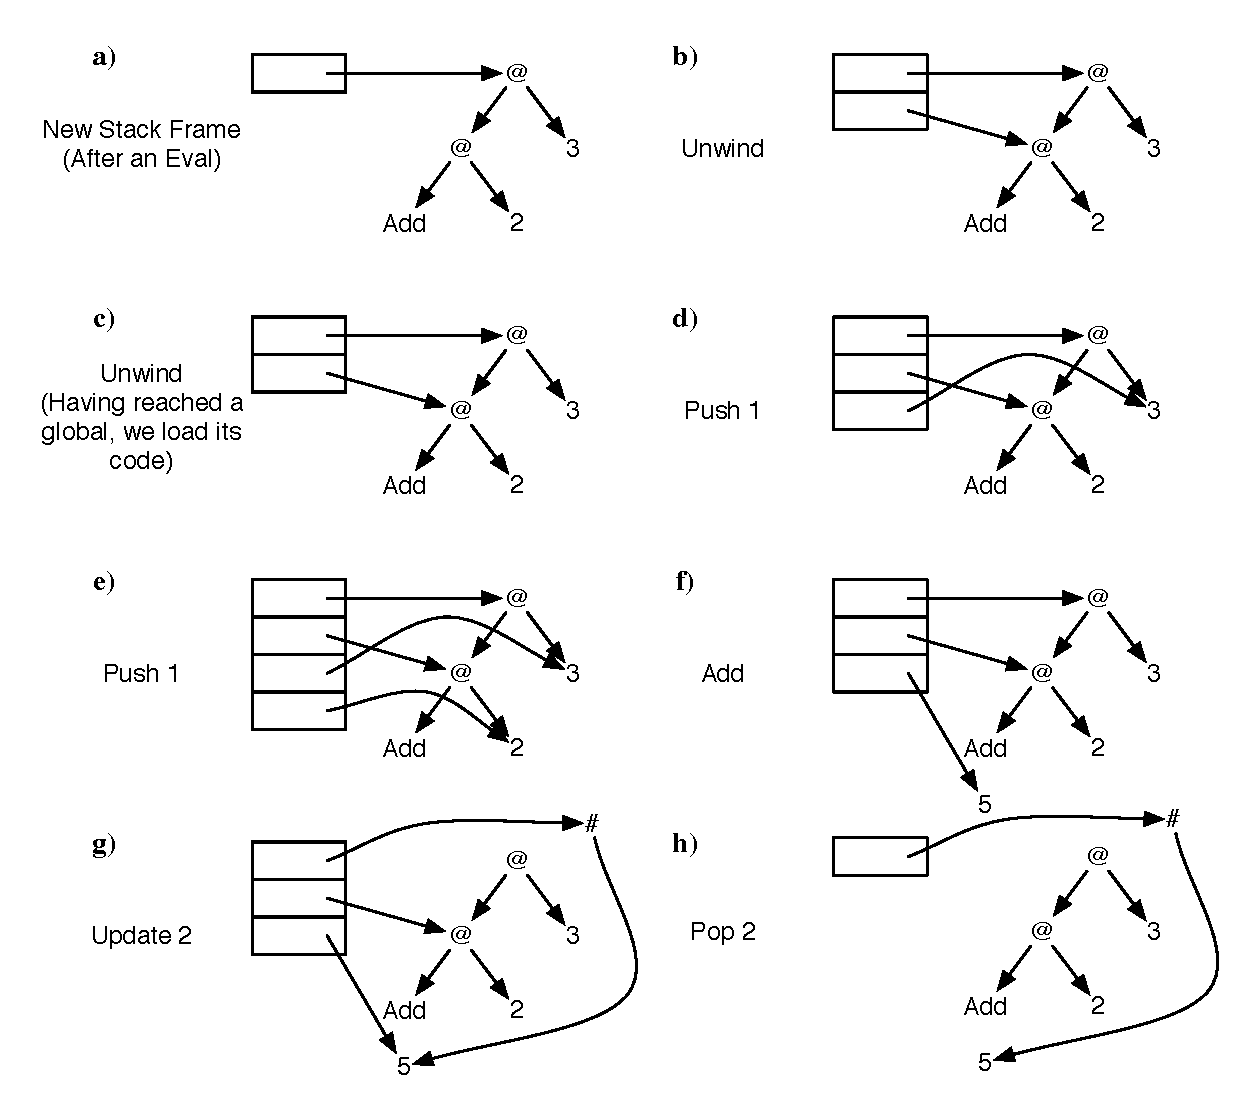
\includegraphics[scale=0.55]{Background/figures/AddExample.eps}
  \caption[G-Code execution example]
   {Walk-through of the \(G\)-Code for Add 2 3}
  \label{example:gCode}
\end{figure}

In figure \ref{example:gCode} we walk through a simple $G$-Machine reduction.
At (a) we have we have a reduction about to take place, the top of the stack is
pointing to the root of the expression. In (b) the GCode instruction Unwind is
executed, placing a pointer to the application node's function argument on the
stack. Unwinding continues until a global function is encountered.
When unwind reaches a global function, as in (c), the $G$-Machine loads
the code for that function and executes it. The code for \verb-Add- is Push 1,
Push 1, Add, Update 2, Pop 2, Unwind\footnote{This version of Add will only work
with primitives as its arguments. In order to accept expressions there would
need to be an Eval instruction added after every Push.}.
The first three instructions are what
actually add the two arguments, with the last three instructions being used to
update the graph and begin unwinding again. Push 1 pushes a pointer to the
argument of the application node pointed to by the address located at stack
address 1 (the stack addressing starts at 0). This is done twice at (d)
and (e) in order to have pointers to both arguments at the top of the stack.
Then we have the Add instruction which dereferences the top two pointers and
adds the resulting values, the resulting value is then pushed onto the stack;
this is seen at (f). With the result now on the stack, updating takes place, (g).
The Update instruction take a value (which is the arity of the function being
evaluated) and updates the stack pointer that originally pointed to the root of
the expression. The pointer is replaced by an indirection node, which is in turn
set to point to the same value as the top stack pointer. With the updating
finished the expression's original graph is no longer needed. Therefore, we can
pop all of the intermediate pointers on the stack, which will always be equal to
the arity of the expression. At (h) we are left with the updated pointer that
can now be used by the calling function. We execute the Unwind instruction again,
entering the $G$-Machine into its unwind state, which will ensure that the
proper stack jumping occurs when there is nothing left to evaluate (such as in
this case).

 \subsection{Spineless $G$-Machine}
    The standard $G$-Machine updates the shared graph after every reduction
step. While this is conceptually simple and easy to implement, such frequent
rewrites in the heap can be seen as wasteful. The Spineless
$G$-Machine improves on this by only updating the graph when loss of sharing is
a possibility \citep{burn1988spineless}. It is known as `spineless' because the
chain of application nodes that would make up the spine in the standard
$G$-Machine is not built up in the heap. Instead it is exclusively
accumulated on the stack until an update is required. The key point in this
variation of the $G$-Machine is that updating should be associated with the
potential loss of sharing and not with a reduction \citep{burn1988spineless}.

    The way this was accomplished was by adding a new type of application node
which they call a ``SAP'' node (for shared application). A SAP node indicates
that the node is `updatable' and that the result of any reduction at that node
should be updated in the graph.

    The mechanism for the updates is slightly different for functions than it is
for values. First let us look at how functions are handled. When a SAP node is
pushed onto the stack during an unwinding a new stack frame is created. When a
pointer outside of the bounds of the stack frame is required we can take this as
a signal that the reduction occurring at the updatable node has resulted in a
function that `fails' the arity test. We then rewrite the subgraph at the SAP
node since we know that sharing could be lost if we continued otherwise.
For values the update is triggered when the value has been reduced to its
base-value form.

    The remaining task for the Spineless $G$-Machine is to determine which
application nodes should be a SAP node, and which should be a standard AP node.
The authors give three different strategies for identifying which nodes should
be marked as SAP. The simplest strategy is that all nodes should be marked as
sharing nodes; this ensures that no sharing will be lost but will find the same
wasteful re-writing that the standard $G$-Machine exhibited. The next strategy
involves simple static sharing analysis to identify the nodes where the
arguments will definitely \emph{not} be shared, so all other nodes are marked as
sharing nodes. Lastly, a dynamic method is suggested that attempts to identify
as few sharing nodes as possible (therefore minimising the re-writing) while
adding an overhead cost of having to check when a shared subgraph is created.
The authors call this mechanism ``dashing'' and argue that the savings of having
as few re-writes as possible make the overhead cost of dashing worthwhile
\citep{burn1988spineless}.


 \subsection{STG-Machine}
    A few years after the design of the Spineless $G$-Machine, another
enhancement was introduced, the Spineless Tagless $G$-Machine. This descendant of
the $G$-Machine is a fully realised Spineless $G$-Machine that eliminates the
need for tagged nodes by using packets\footnote{The original terminology used
for this concept was either a closure, or a thunk; a thunk being a closure that
is fully saturated. However, to differentiate between the \emph{concept} of a
closure and its representation, a packet will refer to the STG-Machine's
representation of a closure.} for its graph representation.

    Each packet consists of a code pointer and zero or more pointer fields used
to point to the values of free variables. The code the packet points to is what
determines the behavior of the node. There is a global \emph{environment
pointer} which addresses a packet, and then the packets code is executed. If
there are any free variables associated with the packet the are accessed via an
offset from the environment pointer \citep{jones1992implementing}. This process
was called `entering' the packet. Because there is no tag on a node, the only
way of determining the purpose of the node is to enter the packet. As said by
Peyton Jones ``each closure (including data values) is represented uniformly,
and scrutinized only by entering it.'' \citep{jones1992implementing}.

    The STG-Machine uses the self-updating model when having to update a
subgraph. Instead of updating after every reduction, like the $G$-Machine, each
packet is responsible for updating itself when an update is necessary. In the
case of a thunk, entering the packet will result in the thunk being overwritten
and the resulting packet's code will simply return the value stored in the
packet.

    The STG-Machine became the basis for GHC and has had many improvements over
the years \citep{HistoryOfHaskell}. Interestingly, one of the improvements to the
STG-Machine was the introduction of tags! The elegance of being able to treat
every node the same has a cost on the performance on modern architectures
\citep{marlow2007faster}.
Because so much of the performance in modern CPUs comes from the speed of its
cache (and therefore avoiding the memory bottleneck) the indirections that arise
from the code pointers in each packet have a significant cost on performance. As
stated in the introduction to their 2007 paper \citep{marlow2007faster}:
\begin{quote}
The tagless scheme is attractive because the code to evaluate a closure is
simple and uniform: any closure can be evaluated simply by
entering it. But this uniformity comes at the expense of performing indirect
jumps, one to enter the closure and another to return to
the evaluation site. These indirect jumps are particularly expensive
on a modern processor architecture, because they fox the branchprediction
hardware, leading to a stall of 10 or more cycles depending on the length of the
pipeline.
\end{quote}

As much as we would like to focus one elegant abstractions and distance
ourselves from the low level concerns, there will always be \emph{some} focus on
performance, and that will sometimes require compromises to accommodate hardware
realities.

    
        \section{Parallel Reduction Machines}
        \label{sec:ParallelMachines}
            Having looked at the $G$-Machine as a sequential abstract machine we can now
look at how graph reduction can occur on parallel architectures. The simplest
parallel variant would be a parallel $G$-Machine. It turns out that once
sequential graph reduction has been accounted for there is not much to add in
order to provide facilities for parallel evaluation. If one were to use a shared
graph almost all communication could take place via that graph.

\begin{figure}[h]
  \centering
  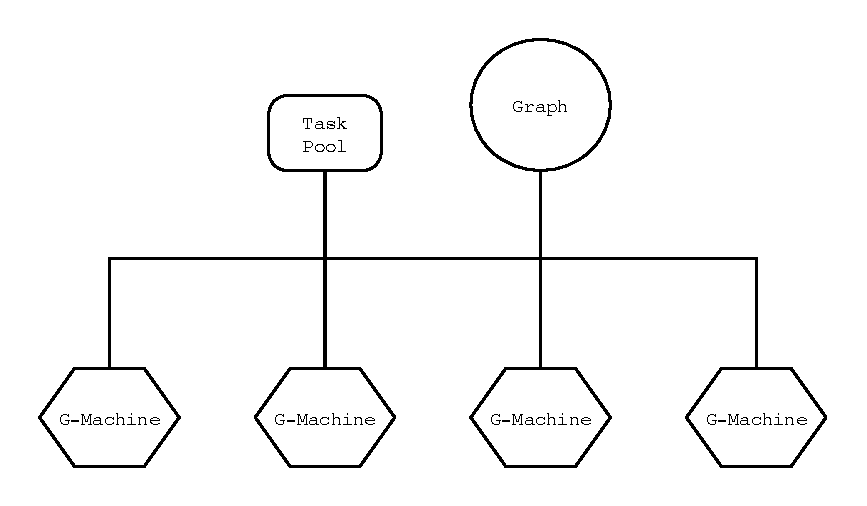
\includegraphics[scale=0.7]{Background/figures/simpleParallel.eps}
  \caption[Simple parallel graph reduction model]
   {A parallel G-Machine}
    \label{fig:simpleGMachine}
\end{figure}

The spark pool is where idle processors can look for subgraphs that have been
sparked off for evaluation. This simple-yet-functioning model is actually the
basis for the implementation described in chapter \ref{chap:platform}
\citep{PeytonJones:IFL}. This model is not specific to the $G$-Machine, but can
be used with any of the graph reduction machines, indeed GHC uses a similar
model that is extended with thread-local heaps \citep{marlow2009runtime}. A
worker thread allocates from its local heap, when a thread's heap has
overflowed the GC stops \emph{all} running threads and moves local-heap data to
the shared heap.

 \subsection{$\langle \nu , G\rangle $-Machine}
    A departure from the stack-based approach of the G-Machine, here we have a
packet-based abstract machine \citep{vGMachine, Alice}.
    The packets (or frame as they are called in the
original paper) are similar to the packets we have seen for the STG-Machine
(although the $\langle \nu , G\rangle $-Machine was described and implemented
first \citep{vGMachine}). One difference is that on top of the code pointer and
pointer to its arguments, there is a dynamic pointer that points to the caller of
the expression the packet represents, and there is a block of free `working
space' on each packet (we will see why in a moment).
The key difference, however, is the way that the
$\langle \nu , G\rangle $-Machine deals with its stack.
As opposed to having a central stack, each packet has its own, using the free
space allocated with the creation of the packet as its local stack.
Therefore the stack for a task is always in
the heap with the task itself \citep{vGMachine}. This is in contrast to the standard
G-Machine, where the stack resides `in' the machine itself and the tasks use
that stack until they are blocked, at which point the task's stack is
transferred to the heap until the task is awoken.
    The $\langle \nu , G\rangle $-Machine avoids any complications of dealing
with the stack by distributing the stack amongst the graph. The stack frame at
any point in the graph is a accessed through the linked list of packets pointing
to their caller.
    One possible way of thinking about this: The traditional stack-based approach has a
stack on each \emph{processor}, whereas the this approach has a stack on
each \emph{process}.

    
        \section{Approaches to Parallelism}
        \label{sec:Approaches}
        When looking at parallel programming, it is important to make the distinction
between concurrency and parallelism.  Concurrency embodies the idea of multiple
workers (threads, computers, agents, etc.) making progress on independent
tasks. A standard example for concurrency is a modern web-server. Each
connection to the web-server can be thought of as an independent sub-task of
the program. The web-server does not have to be run on a multi-core machine for
the concurrency to take place. A single-core machine is capable of running
concurrent threads through scheduling and context switching.

Parallelism describes the simultaneous execution of tasks with the purpose of
achieving a gain in performance. Tasks that can be easily divided into
independent sub-tasks can easily be made into parallel algorithms. For example,
if one wanted to compute the monthly average temperature for a given year, each
month could be computed independently.  If enough of these independent
computations happen simultaneously there can be a substantial improvement in
the program's wall-clock speed. Ideally, the increase in performance would
scale at the same rate as the available parallel machinery (2$x$ performance
with two processors, 5$x$ performance with 5 processors). Unfortunately, there
are some unavoidable factors that prevent this ideal from being realised
\citep{hughes:thesis,HistoryOfHaskell,PFPAnIntro}. The most basic fact
preventing this ideal is that the executing machinery (whether virtual or
physical) will necessarily introduce some overhead in the generation and
management of parallel threads of execution \citep{PeytonJones:IFL}. Beyond
that, it is unusual for a program to be perfectly parallel except in trivial
cases. Most parallel programs exhibit non-uniform parallelism and complex data
dependencies. This results in programs where parallel threads vary greatly in
their processing time and contain threads of execution that will depend on the
results of other threads. This results in threads having to wait for the result
of another thread before commencing (which is known as blocking).

\subsection{Haskell}

Haskell is a lazy functional language benefiting from constant development
since its inception in 1987\footnote{1987 was when the academic community
decided that an `standard' language was needed to unify the study of lazy
functional programming\citep{HistoryOfHaskell}, however, the first Haskell
report was not published until 1990 \citep{Haskell98Book}}
\citep{HistoryOfHaskell, Haskell98Book}. Haskell as defined by the Haskell
Report \citep{Haskell98Book} does not have parallelism as part of the language.
However, functional programming has a long history of parallel implementations
and Haskell is no different in this regard. Even the early implementations of
Haskell had facilities for parallel computation.

\paragraph{Haskell Parallelism}

The Glasgow Haskell Compiler (GHC) has extensive parallelism and concurrency
support, this is part of what makes the compiler a popular implementation
\citep{HistoryOfHaskell}. While our eventual goal is to have access to
compilers that take advantage of the implicit parallelism in our programs, it
is useful to understand the tools and libraries that enable programmers to use
\emph{explicit} parallelism in their Haskell programs. Some of these techniques
are well-established and have decades of use and experience to draw from. Other
techniques are more modern and provide new methods for Haskell programmers to
use parallelism. Often, these newer methods are an `answer' to problems or
pitfalls with the older techniques.

\subsection{Explicit Parallelism with \texttt{par} and \texttt{seq}}

The most popular Haskell compiler, GHC \citep{HistoryOfHaskell}, is able to
compile and run parallel Haskell programs `out of the box'. This ability is
limited to the \emph{shared memory processors}, also known as symmetric
multiprocessors (SMP), that are nearly ubiquitous with the rise of multi-core
architectures in modern CPUs. The GHC project provides several ways to utilise
parallel-capable machines.

The first method is through the \<par\> and \<seq\>\footnote{While
\texttt{seq} was introduced into Haskell for Haskell '98 \citep{Haskell98Book}
it was used for many years before that \citep{HistoryOfHaskell}. One of the
earliest descriptions was by Hughes who introduced a \texttt{synch} combinator
that performed the same function in 1983 \citep{hughes:thesis}.} combinators.
The \<seq\> combinator has the following type.

\begin{haskell}
seq &::& \hasalpha \to \hasbeta \to \hasbeta
\end{haskell}

An expression of the form \<seq a b\> first forces the evaluation of its
first argument to WHNF\footnote{For an expression to be in Weak Head Normal
Form it must be evaluated enough such that the outermost constructor is known.
To say that a function is in WHNF means that the function is partially
applied.} and then returns its second argument. This allows a programmer to
express sequential evaluation. It is important to note that \<seq\> $\bot$
\<b\> results in $\bot$.

It is important to realise that GHC's implementation of \<seq\> is
\emph{not} guaranteed to force the evaluation of its first argument
\emph{before} its second argument. The compiler may find an optimisation that
circumvents the sequencing created by the combinator. In order to provide a
combinator that \emph{does} provide this guarantee GHC provides the
\<pseq\>\footnote{The `p' in \texttt{pseq} stands for parallel.  The idea
being that parallel programs are more likely than sequential programs to
require that \texttt{seq} guarantees its behavior.} combinator.

In the literature, the \<par\> combinator appears in one of two forms
\citep{HistoryOfHaskell, hughes:thesis}. In order to differentiate between the
two forms we will refer to the earlier version as the \emph{applicative} par, or
\<parAp\> and the more recent (and more common) version as \emph{Haskell}
\<par\>\footnote{The reason we will be referring to this as Haskell par is
because most users will know this version of the combinator from their use of
Haskell}.

Haskell \<par\> takes the same form as \<seq\> and has the same type
signature. The combinator takes two arguments, sparks off the first for
evaluation in parallel, and returns the second.

\begin{haskell}
par &::& \hasalpha \to \hasbeta \to \hasbeta \\
par a b &=& b
\end{haskell}

The applicative \<parAp\> expresses a function application whose parameter has been
sparked off to be evaluated in parallel. Semantically, this means that the
applicative par has the following form

\begin{haskell}
parAp &::& (\hasalpha \to \hasbeta) \to \hasalpha \to \hasbeta \\
parAp f x &=& f x
\end{haskell}

% TODO maybe find a place to show this
%The strictness of the function being applied can have a huge effect on the
%parallelism from this combinator. In fact, we will see in section
%\ref{sec:experiments} that in same cases, the compilation of the
%function being applied can have large effects on \verb=parAp='s use.

Interestingly, the version of \<par\> that an implementation chooses does
not change the expressiveness. Each version of \<par\> can actually be
defined in terms of the other. Defining the applicative par in terms of Haskell
par gives us

\begin{haskell}
parAp f x = par x (f x)
\end{haskell}

In order to define Haskell par in terms of applicative par we must use the
\<k\> combinator

\begin{haskell}
k x y &=& x \\
\quad&&\quad \\
par x y &=& parAp (k y) x
\end{haskell}

The benefit of \<parAp\> is that you get the sharing of the parallel computation
without needing to give a name to a subexpression. For example, the following use of
\<parAp\> is very typical.

\begin{haskell}
parAp f (g 10)
\end{haskell}

This does as you would expect, evaluate \<g 10\> and share that with
\<f\>. In order to achieve the same effect using Haskell \<par\> we must
give \<g 0\> a name.

\begin{haskell}
\hslet{x = g 10}{%
       par x (f x)}
\end{haskell}


While language implementors may have strong preferences for one over the other,
there are a few good arguments for the use of Haskell \<par\> Haskell
\<par\> is the simpler of the two versions, using it as an infix combinator
makes it easy to spark an arbitrary number of expressions easily,
\<a `par` b `par` c\>, and the use-case for applicative \<par\> can be easily
expressed using Haskell \<par\>, as shown above.

\todoinline{It may be nice to instrument and profile the quicksort example that comes
    next. Since we have the space to do it, showing how we get a better performing
    algorithm and actually showing the speedups would be insightful.}
\paragraph{Writing a program with \texttt{par} and \texttt{seq}}

Now that we have our essential combinators we are able to define a parallel
algorithm. One of the big sellers of functional programming is the wonderfully
concise Quicksort definition

\begin{haskell}
quicksort &:: (Ord \hasalpha) \Rightarrow [\hasalpha] \to [\hasalpha]\\
quicksort (x:xs) &= less \hsapp x:greater
            \hswhere{less    &= quicksort [y \mid y \hsfrom xs, y \leq x] \\
                     greater &= quicksort [y \mid y \hsfrom xs, y > x]} \\
quicksort \_ &= []
\end{haskell}

The obvious way to parallelise this algorithm is to ensure that each of the two
recursive calls can be executed in parallel, this is a common form of
paralellism known as `divide and conquer' \tocite{Either Hammond or something
earlier}. This can be done by changing the second line to

\begin{haskell}
quicksort (x:xs) = greater `par` (less \hsapp x:greater)
\end{haskell}

The issue with the above is that while the left-hand side is sparked off in
parallel, it will only be evaluated to WHNF if the spark catches. This will
result in only the first \<cons\> of the list. The rest of the list will
only be evaluated if/when \<greater\> is needed\footnote{Because of
laziness it is possible that \texttt{greater} will never be needed. An
example would be if only the head of the sorted list is requested.}. This
fails to exploit all of the parallelism we desire and highlights the sometimes
conflicting nature of parallelism and laziness.

    In order to help us attain the parallelism we are aiming for, we can
introduce a function \<force\> that ensures that its parameters are evaluated
fully. As found in the textbook `Real World Haskell'' \citep{realWorld}

\begin{haskell}
force &:: [\hasalpha] \to ()\\
force list &= force' list `pseq` ()
\hswhere{force' (_:xs) &= force' xs \\
         force' []     &= 1
        }
\end{haskell}

This function takes a list and enforces spine-strictness. As long as the list is
not an infinite structure the use of this function is safe. With this function
in hand we could adapt our basic parallel Quicksort into a better performing one.

An interesting point is that this definition of \<force\> can be much simpler

\begin{haskell}
force &:: [\hasalpha] \to () \\
force (\_:xs) &= force xs\\
force []           &= ()
\end{haskell}

Because the function is fully saturated, the recursive call will continue
evaluating through the entirety of the list. This only goes to show that even
experts sometimes misunderstand when combinators like \<seq\> and \<pseq\> are
needed.

\begin{haskell}
parQuicksort &:: (Ord \hasalpha) \Rightarrow [\hasalpha] \to [\hasalpha]\\
parQuicksort (x:xs) &= force greater `par` (force lesser `pseq` (less ++ x:greater))
\hswhere{less &= parQuicksort [y \mid y \hsfrom xs, y \leq x]\\
         greater &= parQuicksort [y \mid y \hsfrom xs, y > x]
        }
parQuicksort \_ = []
\end{haskell}

Notice that there were a few more changes than just calling \<force\> with
the parallel spark. By also forcing the evaluation of \<lesser\> before
appending the two lists we ensure that both \<greater\> and \<lesser\>
are constructed completely. While this version of a parallel Quicksort does
execute its recursive calls in parallel it has come at a cost. First, the
resulting list is no longer lazy. Using this function for determining the head
of the resulting list would result in the entire list being computed. While
the loss of laziness can sometimes be a worthwhile trade-off (particularly
if the entire list will be required anyway) for an increase in speed, the
second major cost is that this parallel Quicksort does not result in a faster
program!

    Despite the added functions to ensure that laziness did not get in the way
of our desired parallelism, the parallel sorting was actually slower than the
sequential sort. Running a parallel Quicksort on a two core machine, O'Sullivan
found that this algorithm actually resulted in a $23\%$ decrease in
performance \citep{realWorld}. The reason for the slowdown comes up often in the
design of parallel algorithms: There is a minimum amount of work a thread must
perform in order to make the expense of sparking off the thread worthwhile. This
issue highlights what is known as granularity \citep{dutchBook}. While the sparking
of threads is relatively cheap in a system such as GHC, there is still a cost,
and if the amount of work a thread performs is very little, the cost may not be
worth it.

    One way of tackling this issue is by introducing the notion of \emph{depth}
to the function. An additional parameter can be be added to the function that
acts as a count for the depth.

\begin{haskell}
parQuicksort (x:xs) depth = \hsif{depth \leq 0\\}{%
                                  quicksort (x:xs)}{%
                                    else \dots}
\end{haskell}

    In this version we check to see if the desired maximum depth has been
reached and if so then the recursive call is to the standard sequential sorting
algorithm. If the max depth is not reached then we use the body of the
parQuicksort defined above, with the depth argument to each recursive call being
\<depth - 1\> The desired maximum depth is determined by the value given as
the depth argument at the top-level call of the function. This method of
controlling the granularity is a useful one and allows for easy experimentation
on the maximum depth for the problem at hand. The downside is that it
contributes yet another concern for the programmer to worry about.


Managing the granularity of a parallel program is one of the bigger challenges
facing parallel functional programming \citep{SPJ:PIFPL}. Whether decided by
the programmer (with annotations) or by the compiler implicitly, the question
of ``is this task worth it?'' will always come up when deciding what tasks
should be sparked.

\todoinline{To get a really fast quicksort, we'd need to actually implement
    a `real' in place quicksort using something like the ST monad. This would
    be a good spot to discuss the fast that sometimes it's the algorithm that
    is the bottleneck, and not the lack of implicit parallelism.}

\subsection{Explicit Parallelism with the \texttt{Par} Monad}

One of the main benefits of using \<par\> and \<seq\> is that they
provide a simple interface for expressing parallel computation without
the need to worry about concurrency issues such as task/thread creation
and synchronisation. The communication is via the same mechanism that
allows for lazy evaluation \citep{SPJ:PIFPL}. However, laziness can
be difficult to reason about and gaining the maximum benefit from parallelism
can often require the \emph{forcing} of values beyond WHNF. \todo{Reference the forcing in quicksort}
This motivated another approach to deterministic parallelism, the \<Par\>
Monad \citep{marlow2011monad}.

The \<Par\> Monad makes the following trade-off: For the cost of making the
dependencies between computations explicit and prohibiting the use of shared
lazy structures, users gain predictable performance and the ability to reason
about when evaluation takes place. The library provides an API for dataflow
parallelism in Haskell.

Internally the \<Par\> Monad is implemented using I-Structures
\citep{Arvind:IStructures}, which provide the mechanism for communication
between tasks. I-Structures are mutable cells with write-once semantics.
The disciplined use of I-Structures in the \<Par\> Monad are what ensure
deterministic parallelism.


%\footnote{We found that running a similar experiment on a 4-core machine
%did not improve the results by much.}

 \subsection{Implicit Parallelism}
   While explicit parallelism has many advantages and can show great performance
increases, many desire the ability to express a functional program
\emph{without} having to specify where parallelism can take place. This idea,
that parallelism can be achieved without programmer intervention, is known as
implicit parallelism.

  \paragraph{Strictness Analysis}
    Laziness can work against our desire to exploit possible parallelism in
functional programs. Because of this, researchers have discovered that using
static analysis at compile time in order to discover strict portions of a
program can yield promising results. This analysis has been named
\emph{strictness analysis} \citep{ritabook, SPJ:PIFPL}. A trivial example is that
of the addition of two expressions, such as the fibonacci sequence.

\begin{haskell}
nfib n \hsbody{%
            &\mid n \leq 0   &= 0 \\
            &\mid n \equiv 1    &= 1 \\
            &\mid otherwise  &= nfib (n-1) + nfib (n-2)
            }
\end{haskell}

Because the \<(+)\> function is strict in both its arguments we know that
both recursive calls to \<nfib\> will be required. This fact, that we
\emph{know} that the arguments to a function will be required by the function,
is what enables us to exploit the parallelism that is inherent in the program.

    Strictness analysis has
been deemed \emph{conservative} parallelism \citep{SPJ:PIFPL}. This is due to
the idea that sparking an expression that will definitely be required by the
program is not seen as risky. While for the most part this is true, in reality
it depends on how the sparking is handled by the runtime.

    There are also techniques that involve using a program's statistics
    gathered at runtime to better predict where parallelism can be exploited
    \citep{feedbackImplicit}.

\subsection{Semi-Implicit Parallelism with Strategies}
    This section will look at things like `Strategies' to illustrate how a
programmer can write the code they want to write (for the most part) and then
use meta-techniques to make that code parallel.

Strategies came in two waves; the first wave was introduced by Trinder et al. in
"Algorithm \(+\) Strategy \(=\) Parallelism". This incarnation of strategies is
simple to understand and easy to use effectively.

The type declaration for a Strategy is

\begin{haskell}
\hskwd{type} Strategy \hasalpha = \hasalpha \to ()
\end{haskell}

The key point to take away from this is that Strategies do not, and can not,
contribute to the end result of the computation.

It is possible, and useful, to define strategies that do not introduce
parallelism, but instead ensure that evaluation is carried out to some degree.
For example, the strategy for doing nothing

\begin{haskell}
r0 :: Strategy a\\
r0 \_ = ()
\end{haskell}

And for evaluating the argument to WHNF

\begin{haskell}
rwhnf   &:: Strategy \hasalpha\\
rwhnf x &= x `seq` ()
\end{haskell}

These strategies are not often used on their own, but are used in conjunction
with other strategies to achieve a goal. For example, applying a strategy to
each element of a list can be expressed as

\todoinline{fix pagebreak}

\begin{haskell}
seqList &:: Strategy \hasalpha \to Strategy [\hasalpha]\\
seqList strat [] &= ()\\
seqLIst strat (x:xs) &= strat x `seq` (seqList strat xs)\\
\quad&\quad \\
parList &:: Strategy \hasalpha \to Strategy [\hasalpha] \\
parList strat [] &= () \\
parList strat (x:xs) &= strat x `par` (parList strat xs)
\end{haskell}

Both of these functions are common strategies for working on lists. In the first
case, \<seqList\> elements in the list are \emph{sequentially} evaluated
using \<strat\> In \<parList\> each element is evaluated in parallel
using \<strat\> this gives no guarantee of the evaluation order, only that
the sparks will point to each element of the list.

In order to use a strategy, the function \<using\> was defined; taking an
expression and a strategy, it bridges the gap between the specified algorithm
and the desired strategy.

\begin{haskell}
using &:: \hasalpha \to Strategy \hasalpha \to \hasalpha\\
using x s &= s x `seq` x
\end{haskell}

This allows us to define \<parMap\> as

\begin{haskell}
parMap &:: Strategy \hasbeta \to (\hasalpha \to \hasbeta) \to [\hasalpha] \to [\hasbeta]\\
parMap strat f xs &= map f xs `using` parList strat
\end{haskell}

With this we could evaluate all the elements of a list to whatever level the
first argument specifies.

\subsection{Semi-Implicit Parallelism with Skeletons}

There are many cases where the \emph{structure} of two programs in the same
even though they are computing different results. As mentioned above,
\<quicksort\> shares a structure with many algorithms known as `divide and
conquer'. Algorithmic skeletons allow for reuse of \emph{structural} parallelism
between programs \tocite{Algorithmic Skeletons}.

Skeletons are higher-order functions that are passed the computation specific actions
of a program and ensure that the actions are parallelised according to the pre-defined
structural parallelism.

\todoinline{Give an example of a divide and conquer Skeleton}.

\subsection{Semi-Implicit Parallelism via Rewriting}


Some recent work has shown promising results with the use of rewriting. The
programmer uses pre-selected idioms (which is what makes these techniques
semi-implicit) and the compiler uses pre-defined rewrite rules to convert the
high-level idiom to low level parallel code \tocite{The ICFP 2015 paper
``Generating Performance Portable Code using Rewrite Rules: From High-level
Functional Expressions to High-Performance OpenCL Code''}. This technique frees
the programmer from concerning themselves with the low-level optimisation
techniques, which in the case of GPU programming are often vendor specific. The
compiler writers provide different sets of reqrite rules for each target
platform, providing portable parallelism for specific functional idioms.

Another rewriting approach uses a \emph{proof} of the program in seperation
logic \citep{hurlinProof}, to automatically parallelise the program where
it is safe, having the safety guaranteed by the provided proof. The proof can
be transformed as teh program is transformed providing assurance that the
resulting program has the same semantic behavior.

        
        %Review of Graph Reduction. Needs to focus more on the G-Machine and our
        %implementation. Will we convert to spineless G-Machine?
        \section{History of Graph Reduction}
        \section{History of Parallel Graph Reduction}

    1978 Turing Award winner, John Backus, used his acceptance speech to ask the
question: ``Can Programming be liberated from the von Neumann Style?''
\citep{HistoryOfHaskell}. The crux of his argument was that the traditional
and ubiquitous architecture of the day was not suitable for the eventual shift
to parallelism and the performance gains that could be achieved through
parallelism's use. This fed the
interest in novel computer architectures that would more readily support
parallelism.

More declarative languages, and particularly functional languages, were seen as
being better suited to Backus' challenge than more traditional imperative
languages. This is because many imperative languages were designed for the
simplicity of compilation. They free the programmer from repetitive
bookkeeping, such as saving registers for function calls and saving the
intermediate computations in an expression, but do not conceal all aspects of
the underlying machine. Most crucially, they allow arbitrary mutation and
side-effects. This limits the amount of parallelism possible because the result
of a function call can depend on more than values of the passed arguments.

    Work had already been carried out on non-von Neumann architectures
before that time, however, much of it was in the form of abstract machines
that functioned `on top' of the von Neumann architecture \citep{turnerHistory}.

In the early 70's the idea of graph reduction is introduced \citep{wadsworth}
and with it, the concept of lazy evaluation was ready to be formalised.
%\citep{lazyCons, HistoryOfHaskell}
Lazy evaluations has its roots in papers by Henderson and Morris, and Friedman
and Wise \citep{turnerHistory}.  People began to think of ways to better
implement graph reduction machines.  A big breakthrough for software reduction
was Turner's SKI-Combinator reduction scheme in 1979 \citep{turnerHistory,
clackbook}.

    In the 1980's we saw a great interest in parallel architectures for
functional languages. The two main conferences in the field were `LISP and
Functional Programming' (which was held on even years) and `Functional
Programming and Computer Architecture' (which was held on odd years).

    Several novel architectures were developed with the hopes that they could
surpass stock hardware in their performance. This line of research continued
through the 80's and into the early 90's \citep{Alice, GRIP, clackbook,
PFPAnIntro}.

    The G-Machine in '84 showed that lazy functional languages (which had always
been considered inefficient) could be implemented in an efficient manner on
stock hardware. However, the abstract machine could also be used in the
implementations of novel architectures \citep{Augustsson:LazyMLCompiler}.

    The 1990's saw a decline in the amount of research aimed at parallel
functional programming. This was mainly due to the results from earlier research
being less successful than had been hoped (some novel architectures did see good
results, but they could not keep up with the improvements seen in the sequential
hardware sphere) \citep{PFPAnIntro, clackbook}.

    The late 90's and the 2000's saw a resurgence in the interest in parallel
functional programming. While still constrained by the von Neumann bottleneck,
interest in this architecture is high because of the ubiquity of multi-core in
computers today. Generally, many of the techniques discussed earlier are used, but as virtual
machines abstracting away from the hardware architecture (Like GpH using GUM, or
GHC using STG-Machine) \citep{buckwheat, haskellSharedMem}.


While still suffering from the von Neumann bottleneck, the
utilisation of multiple cores has been of increasing interest. This brings us to
today.


\part{The Discovery and Placement of Safe Parallelism}
\label{part:static}

    \chapter{Finding Safe Parallelism}
    \label{chap:discovery} 
    Non-strictness makes it difficult to reason about when expressions are
evaluated. This is due to the fact that call-by-need languages only evaluate
expressions when their results are needed, and when a value is needed can
depend on runtime data. One of the benefits of this approach is that it forces
the programmer to avoid the use of arbitrary side-effects. The resulting purity
means that functions in pure functional languages are \emph{referentially
transparent}, or the result of a function depends only on the values of its
arguments (i.e.  there is no global state that could affect the result of the
function or be manipulated by the function).

Unfortunately this elegant evaluation model is actually at odds with the goals
of performance through parallelism: if we have parallel processing resources,
we wish to use them to do as much work as possible to shorten execution time
\citep{tremblay1995impact}.

Call-by-need semantics forces our compiler to take care in deciding which
sub-expressions can safely be executed in parallel. Having a simple
parallelisation heuristic such as `compute all arguments to functions in
parallel' can alter the semantics of a non-strict language, introducing
non-termination or runtime errors that would not have occurred during a
sequential execution.

The process of determining which arguments are required for a function is known
as \emph{strictness analysis} \citep{mycroft1980theory}. Since the early 1980's
such analysis has been widely used for reducing the overheads of lazy evaluation
\citep{SergeyDemand}. As strictness analysis is a form of termination analysis
it is undecidable in general and therefore any results are approximate. Usually
the abstract semantics are chosen so that the analysis can determine when
an expression is \emph{definitely} needed.

It is possible to throw caution to the wind and \emph{speculate} on which
expressions may be needed. This itself is a rich area of research and requires
the compiler to identify plausible candidates but ensure that errors and
non-termination do not affect the program as a whole \tocite{speculative 
parallelism work}. For our work we chose to utilise only \emph{conservative}
implicit parallelism.

\defineword{Conservative Implicit Parallelism}{The parallelism inherent in
a program from tasks/expressions that would have been evaluated during
the program's sequential execution.}

Conservative parallelism is in line with our overall goal of providing a system
that guarantees that the parallelised program has the same semantics as the
original. Therefore, before we can run our automatically parallelised programs,
we must develop methods and techniques for the compiler to \emph{find} and
\emph{express} the parallelism that is implicit in our programs. Strictness
analysis is suitable in aiding this task but care must be taken in choosing a
specific analysis to use.

This chapter is concerned with studying the alternative analyses and the
trade-offs that are inherent in the differing approaches. A survey of the
concepts and development of strictness analysis will inform our choice of
analysis and allow us to understand the drawbacks and limits of our chosen
method.

\subsection*{Plan of the Chapter}

We provide a high-level overview of the issues and motivations in Section
\ref{sec:strictnessOverview}; this should provide enough context to those who
want to move quickly to the next chapter and not concern themselves with the
details of strictness analysis. The ideas are then expanded in the three
sections that follow. Section \ref{sec:twoPoint} explores basic strictness
analysis using a two-point domain. We will see why a two-point domain results
in an analysis that is too limited for our use in deriving useful parallel
strategies. Using a four-point domain, which we discuss in Section
\ref{sec:fourPoint}, fixes much of this issue and provides much better
information for parallel programs (and has been used toward that end) but does
not allow for analysis on arbitrary data-types. Lastly, we review the work on
projection based analysis, which solves both issues, in Section
\ref{sec:projections}.


        \section{Original Motivation vs. Our Motivation}
        
Purity alone is of huge benefit when dealing with parallelism. Because
functions do not rely on anything but their arguments, the only necessary communication
between threads is the result of the thread's computation, which is
shared via the program's graph using the same mechanism used to implement
laziness \citep{SPJ:PIFPL}.

Laziness, while forcing the programmer to be pure (a boon to
parallelism), is an inherently sequential evaluation strategy. Lazy evaluation
only evaluates expressions when they are \emph{needed}. This is what allows for
the use of infinite data structures; only what is needed will be computed.
This tension between the inherently sequential call-by-need evaluation and the
exploitable parallelism from pure functions is a well known issue
\citep{tremblay1995impact}.

This tension between the call-by-need convention of laziness with parallelism's
desire to evaluate expressions \emph{before} they are needed is well known
\citep{tremblay1995impact}. The most successful method of combating this tension
is through the use of \emph{strictness analysis} \citep{mycroft1980theory,
wadler1987projections, hinze1995projection}.

    
        \section{Overview}
        \label{sec:strictnessOverview}
        Because we are working in a lazy language it is not always safe to evaluate the
arguments to a function before we enter the body of a function. This is easy
to see with a simple example; appending two lists\footnote{Here we have used
the na\"{i}ve recursive version, but any correct version of append will
have the same strictness properties.}:

\begin{verbatim}
    append :: [a] -> [a] -> [a]
    append []     ys = ys
    append (x:xs) ys = x : append xs ys
\end{verbatim}

\verb|append| takes two list arguments, a central question that strictness
analysis asks is: How \emph{defined} must the arguments be to \verb|append|
in order for \verb|append| to terminate?

The first hint is that \verb|append| pattern matches on its first argument.
Because the function must be able to distinguish between a \verb|(:)| and a
\verb|[]| we know that the first argument must be defined \emph{at least} to
the outermost constructor. Therefore a use of \verb|append| that is passed
$\bot$ as its first argument will result in non-termination. What about the
second argument, \verb|ys|? Determining how defined \verb|ys| must be turns
out to be impossible without taking into account the \emph{context} that
a call to \verb|append| occurs in. If the first argument is \verb|[]|
then \verb|ys| must be defined to WHNF. However the \verb|(:)| case
guards the recursive call to \verb|append| and, by extension, the use
of \verb|ys|.

The literature on Strictness Analysis is the story of determining these
properties in the general case. We start in \S \ref{sec:idealAnalysis} with
exploring the simplest Strictness Analysis, \emph{Ideal Analysis} on \emph{flat
domains}. We then show how the work was extended to \emph{non-flat domains} in
\S \ref{sec:4pointDomains}. Lastly, we show how the notion of \emph{contexts}
mentioned above are formalised by the use of \emph{projections} from Domain
Theory in section \ref{sec:projections}.


\subsection{Ideal Strictness Analysis}
\label{sec:idealAnalysis}

However, if a function uses the value of an argument within its body it is safe
to evaluate that argument before, or in parallel to, the execution of the body
of the function. In order to determine which arguments can be evaluated in this
way modern compilers use \emph{strictness analysis} \citep{mycroft1980theory}.
More formally, a function $f$ of $n$ arguments

$$
    f\ x_{1} \dots \ x_{i} \ \dots x_{n} = \dots
$$

\noindent is strict in its $i$th argument if and only if

$$
    f\ x_{1} \dots \ \bot \ \dots x_{n} = \bot
$$

What this states is that $f$ is only strict in its $i$th argument if $f$
becomes non-terminating\footnote{In this paper we use the convention that
$\bot$ represents erroneous or non-terminating expressions.} by passing a
non-terminating value as its $i$th argument.

Knowing the strictness information of a function is the first step in automatic
parallelisation. This is because if $f$ is strict in its $i$th argument we do
not risk introducing non-termination (which would not otherwise be present) by
evaluating the $i$th argument in parallel. In other words, evaluating $x_{i}$ in
parallel would only introduce non-termination to the program if evaluating $f$
with $x_{i}$ would have resulted in $f$'s non-termination anyway.

F-Lite has two primitives for taking advantage of strictness information: $par$
and $seq$.
\begin{figure}
\begin{align*}
    &seq \ :: \ a \rightarrow b \rightarrow b &&par \ :: \ a \rightarrow b \rightarrow b \\
    &seq \ x \ y = y                          &&par \ x \ y = y
\end{align*}
\caption{Semantics of \texttt{seq} and \texttt{par}.}
\label{fig:seqandpar}
\end{figure}

Both functions return the value of their second argument. The difference is in
their \emph{side-effects}. $seq$ returns its second argument only \emph{after}
the evaluation of its first argument. $par$ forks the evaluation of its first
argument in a new parallel thread and then returns its second argument; this is
known as \emph{sparking} a parallel task \citep{clack1986four}.

Strictness analysis was a very active research area in the 1980's and the
development of analyses that provide the type of strictness information
outlined above is a well understood problem \citep{mycroft1980theory,
clack1985strictness, burn1986strictness}.  However, as outlined above,
strictness analysis does not provide satisfactory information about complex
data-structures \citep{wadler1987strictness}. This can be remedied by the
use of \emph{projections} to represent \emph{demand}.

\subsection{Abstract Interpretation}

Mycroft introduced the use of abstract interpretation for performing strictness
analysis on call-by-need programs over thirty years ago
\citep{mycroft1980theory}.
Strictness analysis as originally described by Mycroft was only capable of
dealing with a two-point domain (values that are definitely needed, and values
that may or may not be needed). This works well for types that can be
represented by a flat domain (Integer, Char, Bool, etc.)\footnote{Any type that
can be represented as an enumerated type.} but falls short on more complex data
structures. For example, even if we find that a function is strict in a list
argument, we can only evaluate up to the first \verb'cons' safely. For many
functions on lists, evaluating the entire list, or the spine of the list, is
safe; canonical examples are \verb'sum' and \verb'length'.

In order to accommodate this type of reasoning, Wadler developed a
\emph{four-point domain} for the abstract interpretation of list-processing
programs \citep{wadler1987strictness}. However, when extended in the natural way
for general recursive data structures, the size of the domains made finding
fix-points prohibitively costly.

\section{Projections and Contexts}
\label{sec:projections}

So far our discussion of strictness has only involved two levels of
`definedness': a defined value, or $\bot$. This is the whole story when dealing
with \emph{flat} data-structures such as Integers, Booleans or Enumerations.
However, in lazy languages nested data-structures have \emph{degrees} of
definedness.

Take the following example function and value definitions in F-Lite

\begin{centering}
\begin{BVerbatim}
length []     = 0                   sum []     = 0
length (x:xs) = 1 + length xs       sum (x:xs) = x + sum xs

definedList = [1,2,3,4]             infiniteList = [1,2,3...

partialList = [1,2,bot,4]           loop = loop
\end{BVerbatim}
\end{centering}\\

Both \verb-length- and \verb-sum- are functions on lists, but they use lists
differently. \verb-length- does not use the elements of its argument list.
Therefore \verb-length- would accept \verb-definedList- and \verb-partialList-
(which has a non-terminating element) as arguments and still return the correct
value. On the other hand \verb-sum- \emph{needs} the elements of the list,
otherwise it would not be able to compute the sum. For this reason, \verb-sum-
only terminates if it is passed a fully defined list and would result in
non-termination if passed \verb-partialList-. Neither function would terminate
if passed \verb-infiniteList-, since even \verb-length- requires the list to
have a finite length (some functions do not require a finite list, such as
\verb-head-, the function that returns the first element in a list). With
these examples we say that \verb-length- \emph{demands} a finite list, whereas
\verb-sum- \emph{demands} a fully-defined list.

This additional information about a data-structure is extremely useful when
trying to parallelise programs. If we can determine \emph{how much} of a
structure is needed we can then evaluate the structure to that depth in
parallel.

%The first notable attempt at capturing this type of information was
%by Wadler in 1987 \citep{wadler1987strictness}. However, his approach worked
%well on lists but did not scale well to other, more complex data-structures.

The work that introduced this representation of demands was by Wadler and
Hughes \citep{wadler1987projections} using the idea of \emph{projections} from
domain theory.  The technique we use in our compiler is a projection-based
strictness analysis based on the work in Hinze's dissertation
\citep{hinze1995projection}.  Hinze's dissertation is also a good resource for
learning the theory of projection-based strictness analysis.


\subsection*{Strategies}

With the more sophisticated information provided by projection-based analysis,
we require more than simply $par$ and $seq$. To this end we use the popular
technique of \emph{strategies} for parallel evaluation \citep{strategies,
marlow2010seq}. Strategies are designed to evaluate structures up to a certain
depth in parallel to the use of those structures. Normally, strategies are
written by the programmer for use in hand-parallelised code. In order to
facilitate auto-parallelisation we have developed a method to \emph{derive} an
appropriate strategy from the information provided to us by projection-based
strictness analysis. The rules for the derivation are presented as a
denotational semantics and can be found in our earlier work \citep{calderon}.

\section{The Granularity Problem}

We have now discussed how we find the parallelism that is implicit in our
program, but none of the analysis we provide determines whether the safe
parallelism is \emph{worthwhile}. Often static analysis will determine that a
certain structure is \emph{safe} to compute in parallel, but it is very
difficult to know when it is actually of any benefit. Parallelism has overheads
that require the parallel tasks to be substantial enough to make up for the
cost. A \emph{fine-grained} task is unlikely to require more computation than
the cost of sparking and managing the thread, let alone the potential to
interrupt productive threads \citep{hammond2000research, hogen1992automatic}.

One of the central arguments in our work is that static analysis \emph{alone}
is insufficient at finding both the implicit parallelism and determining whether
the introduced parallelism is substantial enough to warrant the overheads.

Our proposal is that the compiler should \emph{run} the program and use the
information gained from running it (even if it only looks at overall execution
time) to \emph{remove} the parallelism that is too fine-grained. By doing this
we shift the burden of the granularity problem away from our static analysis
and onto our search techniques. This way our static analysis is only used to
determine the safe parallel expressions, and not the granularity of the
expressions.

Here we will describe the method by which we identify the \emph{safe}
parallelism in F-Lite programs and arrange for the evaluation of these
expressions in parallel. The \emph{strictness} properties of a function
determine which arguments are definitely needed for the function to terminate,
whereas the \emph{demand} on an argument tells us \emph{how much} of the
argument's structure is needed. \emph{Strategies} are functions that evaluate
their argument's structure to a specific depth. By analysing the program for
strictness and demand information, we can then generate strategies for the
strict arguments to a function and evaluate the strategies in parallel to the
body of the function. The strategies we generate will only evaluate the
arguments to the depth determined by the demand analysis.

    
        \section{Two-Point Forward Analysis}
        \label{sec:twoPoint}
        As mentioned in the Introduction, the majority of
functional languages use either call-by-need or call-by-value semantics.  While
call-by-need has many attractive properties the delaying of computation incurs
an overhead cost on all computations. Call-by-value, by contrast, has an
execution model that is more easily mapped to conventional hardware, allowing
for simpler implementations that achieve good performance \tocite{SPJ or
someone}. Mycroft used this tension to motivate his development of strictness
analysis \citep{mycroft1980theory}:

\begin{displayquote}

The above arguments suggest that call-by-value is more efficient but
call-by-need preferable on aesthetic/definedness considerations. So techniques
are herein developed which allow the system to present a call-by-need interface
to the user but which performs a pre-pass on his program annotating those
arguments which can validly be passed using call-by-value.

\end{displayquote}

By determining which arguments can be safely passed using call-by-value
we diminish the overhead of call-by-need, paying the overhead of
suspending computation only when necessary to ensure that call-by-need
semantics are maintained.

While this was the original motivation for strictness analysis it also serves
in identifying potential parallelism in a program. When an argument is suitable
to be passed as call-by-value it is also suitable to be evaluated in parallel.
In this case the value is evaluated in parallel to the original thread.
Synchronisation is accomplished via the same mechanism as laziness, with the
exception that a thread can be blocked while waiting for another thread to
complete its evaluation.

\subsection{Safety First}

Strictness analysis is chiefly concerned with \emph{safety}. In order to retain
the origin call-by-need semantics the runtime can only alter the evaluation order
when doing so guarantees the same termination properties of the program.

We will refer to this notion of safety as the \emph{strictness} properties
of an argument. Take a function $f$ of $n$ arguments

\begin{equation*}
f \ x_{1} \ \dots x_{i} \ \dots \ x_{n} \ = \langle \texttt{function body} \rangle
\end{equation*}

The $i$th argument of $f$ is said to be strict \emph{if and only if}

\begin{equation}
f \ x_{1} \ \dots \bot_{i} \ \dots \ x_{n} \ =  \bot
\end{equation}
\label{eq:idealSafety}

For any possible values of $x_{1}-x_{i-1},x_{i+1}-x_{n}$.

Equation \ref{eq:idealSafety} can be read as ``$f$ is strict in $x_{i}$ when $f$
fails to terminate if $x_{i}$ fails to terminate''. The reason this allows us
to evaluate the $i$th argument before it is needed is because doing so would only result
in introducing non-termination if the program would have resulted in non-termination
otherwise.

\subsection{Abstract Domains}

Now that we have established what it means to be strict we can expand on how we
analyse programs for this property. As with any abstract interpretation,
this involves the choice of an abstract domain.

%% Hasse diagram for the flat domain of integers.
%%
%% We have a horizontal 'number line' from -infity to infinity and edges from each
%% number to _|_ which is centered below the numbers.
\begin{figure}[!h]
\centering
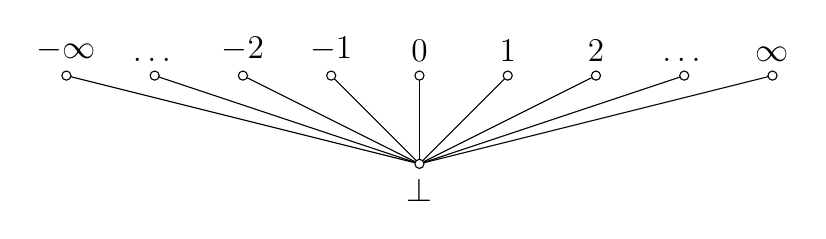
\begin{tikzpicture}
    \node [hasse, label=above:\large$0$]                (zero) at (0,0) {};
    \node [hasse, right = of zero, label=above:\large$1$] (one)   {};
    \node [hasse, right = of one, label=above:\large$2$]  (two)   {};
    \node [hasse, left = of zero, label=above:\large$-1$]  (neg1)  {};
    \node [hasse, left = of neg1, label=above:\large$-2$]  (neg2)  {};
    \node [hasse, left = of neg2, label=above:\large$\dots$]  (ldots) {};
    \node [hasse, right = of two, label=above:\large$\dots$]  (rdots) {};
    \node [hasse, left = of ldots, label=above:\large$-\infty$] (nInf)  {};
    \node [hasse, right = of rdots, label=above:\large$\infty$](inf)   {};

    \node [hasse, below = of zero, label=below:\large$\bot$] (bot)   {};

    \draw[black] (zero) -- (bot);
    \draw[black] (one) -- (bot);
    \draw[black] (two) -- (bot);
    \draw[black] (neg1) -- (bot);
    \draw[black] (neg2) -- (bot);
    \draw[black] (ldots) -- (bot);
    \draw[black] (rdots) -- (bot);
    \draw[black] (inf) -- (bot);
    \draw[black] (nInf) -- (bot);
\end{tikzpicture}
\caption{Flat Domain}
\label{fig:flatInts}
\end{figure}

In non-strict languages types like Integers and Booleans form a flat domain;
either we have a value of that type, or we have $\bot$. This is depicted in
Figure \ref{fig:flatInts}. We can form an intuition of these orderings by
thinking about how much we \emph{know} about a certain value. While the
interger value $5$ maybe greater than the integer value $4$, we know the
same amount about each of them: their values. However, if we have a procedure
that is meant to compute an integer, and therefore has the type \<Int\>, and it
loops forever, we cannot know that Integer's value. Therefore we know less
about a non-terminating value.


This fits nicely with call-by-need semantics: an argument to a function of
type \<Int\> is really a computation that can either result in a value, or
result in non-termination. In terms of strictness analysis, this allows us to
abstract our real domain of Integers to the simple two-point domain shown in
figure \ref{fig:twoPointNice}.

This is the domain we use for basic strictness analysis. The bottom of the
lattice, $\bot$, as implied above, represents \emph{definitely non-terminating}
expressions. The top of the lattice, $\top$, is used to represent
\emph{potentially terminating}\footnote{Remember that program analysis must
approximate in the general case.} expressions. This approximation can seem
counterintuitive; why are we allowing the analysis to say some results are
potentially terminating when they could be non-terminating? The reasoning is
that non-termination is okay under non-strict semantics! If we approximated in
the opposite direction (as analyses for other purposes sometimes do) we may
accidentally compute a value that was never needed, defeating the purpose of
call-by-need evaluation.


\begin{figure}[hb]
\centering
\begin{tikzpicture}
    \node [hasse, label=above:\large$\top$]                 (top) {};
    \node [hasse, below = of top, label=below:\large$\bot$] (bot) {};

    \draw[black] (top) -- (bot);
\end{tikzpicture}
\caption{Two-point Domain}
\label{fig:twoPointNice}
\end{figure}

\subsubsection{Abstracting Functions}

Now that we know what it means to be strict and why we represent flat domains
as a two-point domain the next step is to abstract the functions in our
program. 

The idea is simple: for every function in our program of type \<A\> we must
produce a function of type \<A^{\#}\> that works on the abstracted
values\footnote{Some texts represent an abstracted type by a number \<N\> where
$N$ is the number of points in the abstract domain. We prefer to retain the
context of where this abstract domain came from.}. This abstracted program
is then interpreted using an abstract semantics that provides us with the
strictness information for each function in our program.

\todoinline{standard abstract interpretation diagram}


While this separation of abstracting the program and then performing an
abstract interpretation is useful from the theoretical point of view, many
compilers skip the intermediate representation of an abstracted program and
perform the abstract interpretation with the original AST
\citep{hinze1995projection, kubiak, SergeyDemand}.

We begin with the set of primitive arithmetic functions. In the case of F-Lite,
each numeric primitive is strict in both arguments, providing us with the
following for each of \<(+), (-), (*), (/)\>:

\begin{haskell*}
(\(\odot\)) &::& Int^{\#} -> Int^{\#} -> Int^{\#} \\
\(\top\) \(\odot\) \(\top\) &=& \(\top\) \\
\(\top\) \(\odot\) \(\bot\) &=& \(\bot\) \\
\(\bot\) \(\odot\) \(\top\) &=& \(\bot\) \\
\(\bot\) \(\odot\) \(\bot\) &=& \(\bot\)
\end{haskell*}

We must also be able to combine results from different paths in a program. This
requires both conjunction and disjunction. We can use the \<meet\> ($\sqcap$)
and \<join\> ($\sqcup$) from our lattice which are fully described in Figure
\ref{fig:twopointMeet}.

\begin{figure}
\centering
\begin{minipage}{.5\textwidth}
\begin{haskell*}
\(\top\) \(\sqcap\) \(\top\) &=& \(\top\) \\
\(\top\) \(\sqcap\) \(\bot\) &=& \(\bot\) \\
\(\bot\) \(\sqcap\) \(\top\) &=& \(\bot\) \\
\(\bot\) \(\sqcap\) \(\bot\) &=& \(\bot\)
\end{haskell*}
\end{minipage}
\quad\quad
\begin{minipage}{.5\textwidth}
\begin{haskell*}
\(\top\) \(\sqcup\) \(\top\) &=& \(\top\) \\
\(\top\) \(\sqcup\) \(\bot\) &=& \(\top\) \\
\(\bot\) \(\sqcup\) \(\top\) &=& \(\top\) \\
\(\bot\) \(\sqcup\) \(\bot\) &=& \(\bot\)
\end{haskell*}
\end{minipage}
\caption{The \emph{meet} ($\sqcap$) and \emph{join} ($\sqcup$) for our lattice}
\label{fig:twopointMeet}
\end{figure}

We can now define an abstract interpretation, $\mathcal{A}$, that takes
expressions in our language and gives us their abstracted values. We require an
environment that maps variables and functions to abstracted values, we use,
\<\hasphi :: Id \to Exp^{\#}\> to represent this environment. We write
\<\hasphi[x \mapsto v]\> to represent extending the environment with identifier
\<x\> being mapped to the value \<v\>. Lastly, looking up a value in the environment
is just applying the environment to the identifier.

\begin{figure}
\begin{haskell*}
\mathcal{A} &::& Exp \to Env^{\#} \to Exp^{\#} \\
%
\mathcal{A}\Sem{Var v} \hasphi &=& \hasphi v \\
%
\mathcal{A}\Sem{Int i} \hasphi &=& \(\top\) \\
%
\mathcal{A}\Sem{Con c} \hasphi &=& \(\top\) \\
%
\mathcal{A}\Sem{Fun f} \hasphi &=& \hasphi f\\
%
\mathcal{A}\Sem{App (Fun f) [a_{1}, \dots a_{n}]} \hasphi &=&
        \mathcal{A}\Sem{f} \hasphi (\mathcal{A}\Sem{a_{1}} \hasphi) \dots
        (\mathcal{A}\Sem{a_{n}} \hasphi)\\
%
\mathcal{A}\Sem{Let b_{1} = e_{1} \(\dots\) b_{n} = e_{n} in e} \hasphi &=&
        \mathcal{A}\Sem{e} \hasphi[b_{i} \(\mapsto\) \mathcal{A}\Sem{e_{i}}] \\
%
\mathcal{A}\Sem{Case e alts}    \hasphi &=& \mathcal{A}\Sem{e} \hasphi
        \(\sqcap\) \mathcal{C}\Sem{alts} \hasphi \\
%
\quad&\quad&\quad \\
%
\hsnoalign{\mathcal{C}\Sem{c_{1}\ vars_{1} \to e_{n}, \(\dots\), c_{n}\ vars_{n} \to e_{n})} \hasphi =
        e^{\#}_{1} \(\sqcup \dots \sqcup\) e^{\#}_{n}
        \hswhere{%
            e^{\#}_{1} &= \mathcal{A}\Sem{e_{1}} \hasphi[vars_{1} \(\mapsto \top\)] \\
            & \vdots \\
            e^{\#}_{n} &= \mathcal{A}\Sem{e_{n}} \hasphi[vars_{i} \(\mapsto \top\)]
        }
        }
\end{haskell*}
\caption{An Abstract Semantics for Strictness Analysis on a Two-Point Domain}
\label{fig:twoPointAI}
\end{figure}

%\todoinline{Fix rule C so that we take into account the vars introduced by case
%alternatives (they should all be approximated as Top)}

\subsection{Some Examples}

We can now use the abstract semantics from Figure \ref{fig:twoPointAI} on some
real functions.

\subsubsection{The Constant Function:}

The function \<const\> is defined as

\begin{haskell*}
const x y = x
\end{haskell*}

For non-recursive functions, like \<const\>, we can determine the strictness
properties fully with just $n$ iterations of $\mathcal{A}$ where $n$ is the
number of arguments to the function. We run the abstract interpretation using
$\bot$ as the value for the argument we are currently interested in and $\top$
for all the rest.

First we analyse \<x\>:
\begin{haskell*}
\mathcal{A}\Sem{x}[x \mapsto \(\bot\), y \mapsto \(\top\)] \Rightarrow \(\bot\)
\end{haskell*}

then \<y\>:
\begin{haskell*}
\mathcal{A}\Sem{x}[x \mapsto \(\top\), y \mapsto \(\bot\)] \Rightarrow \(\top\)
\end{haskell*}

Remembering what it means to be strict from Equation \ref{eq:idealSafety}, this
analysis tells us that \<const\> is strict in \<x\> but not in \<y\>. This is
exactly what we would expect.

\hfill$\Box$

\subsubsection{Conditional}

In non-strict languages we can define our own control-flow abstractions,
allowing what is usually a primitive, the \<if\> statement, to be defined
naturally in the language as

\begin{haskell*}
if p t e = \hscase{p}{\\
                      True \to t\\
                      False \to e}
\end{haskell*}

Analysing \<if\> should determine that is strict in \<p\>

\begin{haskell*}
\mathcal{A}\Sem{Case\ p\  [True \to t, False \to e]} \hasphi
\hsbody{%
    \quad& \Rightarrow \mathcal{A}\Sem{p} \hasphi \(\sqcap\)
        (\mathcal{A}\Sem{t} \hasphi \(\sqcup\)
         \mathcal{A}\Sem{e} \hasphi)\\
    \quad& \Rightarrow \(\bot \sqcap (\top \sqcup \top)\)\\
    \quad& \Rightarrow \(\bot\)
}
\hswhere{%
\quad \hasphi = [p \mapsto \(\bot\),t \mapsto \(\top\), e \mapsto \(\top\)]
}
\end{haskell*}

This shows how the use of \<meet\> and \<join\> are used to combine the
results from the different branches of the function. Because the discriminant
of a \<Case\> expression is always evaluated to WHNF, a non-terminating
discriminant results in a non-terminating function.

Notice that if we analysed the second two arguments to \<if\> then we would
have seen that they are not strict for \<if\> because only one would be $\bot$
at a given time and \<meet\> ($\sqcup$) only results in bottom if both arguments
are bottom.


\hfill$\Box$

\subsubsection{Calling Abstract Functions}

Calling functions in the abstract interpretation is the same as a function
call in the standard interpretation except that the target of the call is
the abstracted function. Dependency analysis is used to ensure that callees
are analysed before their callers. The following example illustrates calling
functions and the fact that the abstraction of \<Case\> is capable of determining
when an argument is needed in all the branches.


\begin{haskell*}
addOrConst b x y = \hscase{b}{\\
    True \to x + y\\
    False \to x
    }
\end{haskell*}

The analysis for the second argument proceeds as follows

\pagebreak

\begin{haskell*}
\mathcal{A}\Sem{Case\ b\  [True \to x + y, False \to x]} \hasphi
\hsbody{%
    \quad& \Rightarrow \mathcal{A}\Sem{b} \hasphi \(\sqcap\)
        (\mathcal{A}\Sem{x + y} \hasphi \(\sqcup\)
         \mathcal{A}\Sem{x} \hasphi)\\
    \quad& \Rightarrow \(\top\) \(\sqcap\)
        (\mathcal{A}\Sem{x + y} \hasphi \(\sqcup\)
         \mathcal{A}\Sem{x} \hasphi)\\
    \quad& \Rightarrow \(\top\) \(\sqcap\)
        ((\mathcal{A}\Sem{+} \hasphi (\mathcal{A}\Sem{x} \hasphi) (\mathcal{A}\Sem{y} \hasphi)) \(\sqcup\)
         \(\top\))\\
    \quad& \Rightarrow \(\top\) \(\sqcap\)
        ((+^{\#} \(\bot\) \(\top\)) \(\sqcup\)
         \(\top\))\\
    \quad& \Rightarrow \(\top \sqcap (\bot \sqcup \top)\)\\
    \quad& \Rightarrow \(\bot\)
}
\hswhere{%
\quad \hasphi = [b \mapsto \(\top\),x \mapsto \(\bot\), y \mapsto \(\top\)]
}
\end{haskell*}

The other language constructs are interpreted similarly. Do note that we do not
attempt to analyse functions with free variables. Instead we take advantage of
lambda-lifting in order to remove nested functions to the top level. We are not
the first to use lambda lifting in order to avoid this problem
\citep{clack1985strictness}. Luckily, lambda lifting is done regardless for
compilation to the $G$-Machine.

\hfill$\Box$


\subsubsection{Recursive Functions}

Our last concern is with recursive functions. We use the fact that recursive
abstract functions are just recursive functions on a different domain. This
allows us to define a recursive function as the least upper bound of successive
approximations of the function, i.e. an \emph{ascending Kleene chain} (AKC).

We calculate this by starting with the `bottom' approximation where all sets of
inputs are mapped to $\bot$. For a function $f$ we call this $f^{\#0}$. We then
calculate $f^{\#n}$ by replacing each call to $f$ with $f^{\#(n - 1)}$. This
series of successive approximations forms the AKC.

So for a function of the form

\begin{haskell*}
f x_{1} \dots x_{m} = \hsinf{body of \<f\> which includes a call to \<f\>}
\end{haskell*}

We generate the following AKC

\begin{haskell*}
f^{\#0} x_{1} \dots x_{m} &=& \(\bot\) \\
f^{\#1} x_{1} \dots x_{m} &=& \hsinf{body of \<f\> with call to \<f^{\#0}\>} \\
f^{\#2} x_{1} \dots x_{m} &=& \hsinf{body of \<f\> with call to \<f^{\#1}\>} \\
f^{\#3} x_{1} \dots x_{m} &=& \hsinf{body of \<f\> with call to \<f^{\#2}\>} \\
\quad &\vdots& \quad \\
f^{\#n} x_{1} \dots x_{m} &=& \hsinf{body of \<f\> with call to \<f^{\#(n - 1)}\>}
\end{haskell*}

We can stop the calculation of this AKC when $f^{\#n} \equiv f^{\#(n - 1)}$ for
\emph{all combinations} of $x_{1}$ to $x_{m}$. This means that for each iteration
of the AKC we must interpret $f$ $2^m$ times!

Fortunately, there are clever ways of avoiding much of this expense for the average
cases. Clack and Peyton Jones developed an algorithm for the efficient
calculation of an AKC \citep{clack1985strictness}.

\hfill$\Box$

\subsubsection{Discussion of Two-Point Strictness Analysis}

We have now seen how to use rule $\mathcal{A}$ from Figure \ref{fig:twoPointAI}
to analyse functions in our programs. Now we can see how the results help us in
our ultimate aim of implicit parallelism. For this discussion we will forget
that parallelism is not always beneficial and focus on how we would utilise
all possible parallelism.

Imagine we have a function $f$ with a call to $g$ in its body.

\begin{haskell*}
f \dots = \dots g e_{1} e_{2} e_{3} \dots
\end{haskell*}

Our analysis may determine that $g$ is strict in its first two arguments,
providing us with an opportunity for parallelism. This would allow us
to safely rewrite $f$ as the following

\begin{haskell*}
f \dots = \dots \hslet{x &= e_{1}\\
                       y &= e_{2}
                       }{%
                       x `par` y `par` g x y e_{3} \dots
                       }
\end{haskell*}

The expressions $e_{1}$ and $e_{2}$ are bound to the names $x$ and $y$
in a \<let\> expression so that the results of parallel evaluation are
shared with the body of $g$.

As mentioned above, the two-point domain informs us about strictness up to
WHNF. So if $e_{1}$ or $e_{2}$ are values from a flat domain, this
transformation will provide all the benefits possible to $g$\footnote{Again,
ignoring the fact that it may not actually be a positive benefit.}. But what if
these arguments are of a non-flat type, like pairs or lists?

Because we aim for safe parallelism, we cannot evaluate $e_{1}$ or $e_{2}$ any
further than WHNF, already eliminating a vast quantity of potential parallelism.
Take the function \<sum\> for example:

\begin{haskell*}
f \dots = \dots \hslet{xs &= e_{1}
                       }{%
                       xs `par` sum xs \dots
                       }
\end{haskell*}

When a programmer wants to express this idiom in their code they often use
\emph{parallel strategies} as illustrated in Section \ref{sec:Approaches}.
This allows the programmer to write an expression similar to \<xs `using`
parList\>. This forces the evaluation of the list beyond WHNF. Because our
two-point domain does not guarantee the safety of evaluating beyond WHNF we are
not able to use a strategy like \<parList\>. This means that even though we
`know' that \<sum\> requires the list fully, the analysis has no way to
represent this, and can only determine that the outermost constructor is
needed!

Because of this shortcoming, strictness analysis in this form is inappropriate
for discovering the parallelism in a program that uses nested structures. In
the next section we will see how this deficiency is overcome by choosing
suitable domains for non-flat structures.

%
%data Exp &=& App Exp [Exp] \\ &|& Case Exp [Alt] \\ &|& Let [Binding] Exp \\
%&|& Fun Id \\

    
        \section{Four-Point Forward Analysis}
        \label{sec:fourPoint}
        As noted in the last section, two-point domains are quite limited when dealing
with lazy structures. A more formal explanation for this limitation is that the
two-point domain really represents reduction to WHNF or $\bot$, and nothing
else. In the case of flat domains this is sufficient because WHNF is all there
is. For nested data types the reality is much different. 

For functions that work on lists, like \<sum\> or \<append\>, strictness up to
WHNF is not much benefit. Strictness analysis as described in the previous
section would be able to tell us that \<sum\> requires its argument to be
defined, allowing us to evaluate it before entering the function (or in
parallel). But it is only safe up to WHNF. Once the first \<Cons\> is reached
we must stop evaluation of the list or risk introducing non-termination.
Through the lens of implicit parallelism it seems that we are unlikely to
benefit from introducing parallel evaluation when we are limited to
WHNF\footnote{Indeed most uses of the basic strictness information were for
improving the code generation to avoid building unnecessary suspensions.}. This
is clearly a problem.

The solution seems clear: we must extend the abstract domains for non-flat data
types so that we can have more detailed strictness information. For some data
types, extending the technique is straightforward. In F-Lite, pairs can be
defined as follows.

\begin{haskell*}
data Pair \hasalpha \hasbeta = MkPair \hasalpha \hasbeta
\end{haskell*}

Many languages, such as Haskell, Clean, and the ML family provide the following
syntactic sugar for pairs (and other $N$-tuples): \<(\hasalpha,\hasbeta)\>.

A first try at representing pairs of values from the two-point domain could
give us the lattice in Figure \ref{fig:unboxedPairs}.

\captionsetup[figure]{format=fnoline}
\begin{figure}
\centering
\begin{subfigure}{0.4\textwidth}
\begin{tikzpicture}
    \node [center] (cent) {};
    \node [hasse, above = of cent, label=above:{\large\<(\(\top\),\(\top\))\>}]  (top)   {};
    \node [hasse, left = of cent, label=left:{\large\<(\(\top\),\(\bot\))\>}]    (left)  {};
    \node [hasse, right = of cent, label=right:{\large\<(\(\bot\),\(\top\))\>}]  (right) {};
    \node [hasse, below = of cent, label=below:{\large\<(\(\bot\),\(\bot\))\>}] (bot)   {};

    \draw[black] (top) -- (left);
    \draw[black] (top) -- (right);
    \draw[black] (right) -- (bot);
    \draw[black] (left) -- (bot);
\end{tikzpicture}
\caption{Unlifted Pairs}
\label{fig:unboxedPairs}
\end{subfigure}
\hfill
\begin{subfigure}{0.4\textwidth}
\begin{tikzpicture}
    \node [center] (cent) {};
    \node [hasse, above = of cent, label=above:{\large\<(\(\top\),\(\top\))\>}]  (top)   {};
    \node [hasse, left = of cent, label=left:{\large\<(\(\top\),\(\bot\))\>}]    (left)  {};
    \node [hasse, right = of cent, label=right:{\large\<(\(\bot\),\(\top\))\>}]  (right) {};
    \node [hasse, below = of cent, label=315:{\large\<(\(\bot\),\(\bot\))\>}] (bot)   {};
    \node [hasse, below = of bot, label=below:{\large$\bot$}] (Bot)   {};

    \draw[black] (top) -- (left);
    \draw[black] (top) -- (right);
    \draw[black] (right) -- (bot);
    \draw[black] (left) -- (bot);
    \draw[black] (bot) -- (Bot);
\end{tikzpicture}
\caption{Lifted Pairs}
\label{fig:boxedPairs}
\end{subfigure}
\caption{Domain for pairs of flat-domain values}
\hrulefill
\end{figure}
\captionsetup[figure]{format=myformat}

The meaning of this lattice is fairly intuitive. When we possess a pair of
flat-domain values there are four possibilities, we can have

\begin{enumerate}
    \item The pair structure itself (\<MkPair\>), but accessing either value
        results in non-termination
    \item The pair structure itself, but accessing the \<fst\> element 
        results in non-termination
    \item The pair structure itself, but accessing the \<snd\> element
        results in non-termination
    \item The pair structure itself and both values are fully defined
\end{enumerate}

Notice that possibilites 2 and 3 are similar in that there are one defined and
one undefined item in each. Suggesting that one of 2 or 3 is more defined than
the other would make little sense.  For this reason we say that they are
\emph{incomparable}, i.e. they are neither more nor less defined than each
other.

However, the lattice in Figure \ref{fig:unboxedPairs} is only valid for
\emph{unlifted} pairs, where the constructor value, \<(,)\>, is always defined.
The reality for non-strict languages is that \emph{any} value may be undefined,
including the constructors for product types.

This means that we must \emph{lift} the domain, adding a further bottom value
that represents a failure to construct the pair's outermost constructor
(\<MkPair\> in the F-Lite case). The result, shown in Figure
\ref{fig:boxedPairs}, is typical of domains for strictness analysis on finite
types. You can construct an appropriate domain assuming that the structure is
itself defined, then lift the resulting lattice with an additional $\bot$ that
represents a failure to construct the structure.

Because this domain is still finite we are able to incorporate it into the
framework developed by Mycroft without much issue, simply defining the
appropriate \<meet\> and \<join\> on the lattice and the strictness properties
for any primitives that work with pairs. The main issue is that extending the
technique to non-flat domains in the obvious way introduces infinite domains
for recursive types, losing a lot of the power of abstract interpretation
\tocite{John Hughes work on non-flat domains before wadler and mycroft's thesis
pg 82}.

The first practical solution was proposed by Wadler involving a four-point
domain for lists \citep{wadler1987strictness}. Instead of representing the
recursive structure of lists directly, which creates an infinite domain, Wadler
chose a domain that represents four degrees of definedness for lists.

\begin{figure}[t]
\centering
\begin{tikzpicture}
    \node [hasse, label=above:{\large$\top_{\in}$}]                   (full)   {};
    \node [hasse, below = of full, label=right:{\large$\bot_{\in}$}]  (finite) {};
    \node [hasse, below = of finite, label=right:{\large$\infty$}]    (inf)    {};
    \node [hasse, below = of inf, label=below:{\large$\bot$}]         (bot)    {};

    \draw[black] (full) -- (finite);
    \draw[black] (finite) -- (inf);
    \draw[black] (inf) -- (bot);
\end{tikzpicture}
\caption{Wadler's Four-point Domain}
\label{fig:listDomain}
\end{figure}

The result, as shown in Figure \ref{fig:listDomain}, can be described, from least
to most defined as follows:

\begin{enumerate}
    \item $\bot$ represents all undefined lists
    \item $\infty$ represents all undefined lists, lists  with undefined tails
        and all infinite lists
    \item $\bot_{\in}$ represents all of the above in addition to all finite
        lists with at least one undefined element
    \item $\top_{\in}$ represents fully defined lists along with all of the above
\end{enumerate}


Because we are now concerning ourselves with values from different domains in
our analysis we must now know the types of expressions in our program. This
ensures that we do not accidentally try to \<meet\> or \<join\> values from
different domains. 

To incorporate the four-point domain into the abstract interpretation from the
previous section we need a few new primitives. The \<Cons\> constructor is
given the abstract definition shown in Figure \ref{fig:cons4}. \<Nil\>, being a
fully defined list, is always abstracted as $\top_{\in}$.  There are a few
points worth mentioning about the definition of \<cons^{\#}\>.  First, none of
the equations result in $\bot$.  This makes sense with our understanding of
lazy evaluation, if we have the outermost constructor we have a value in WHNF
and therefore it is definitely \emph{not} $\bot$. Additionally, notice that
\<cons\>ing a defined value onto $\bot_{\in}$ also results in $\bot_{\in}$,
this keeps \<cons^{\#}\> monotonic in addition to aligning with our intuitions
(\<cons\>ing a defined element to the beginning of a list with possibly
undefined elements does not suddenly make the list fully defined). 

\begin{figure}
\centering
\begin{minipage}{.5\textwidth}
\begin{haskell*}
cons^{\#} \(\top\) \(\top_{\in}\) &=& \(\top_{\in}\) \\
cons^{\#} \(\top\) \(\bot_{\in}\) &=& \(\bot_{\in}\) \\
cons^{\#} \(\top\) \(\infty\)     &=& \(\infty\) \\
cons^{\#} \(\top\) \(\bot\)       &=& \(\infty\) \\
\end{haskell*}
\end{minipage}
\quad\quad
\begin{minipage}{.5\textwidth}
\begin{haskell*}
cons^{\#} \(\bot\) \(\top_{\in}\) &=& \(\bot_{\in}\) \\
cons^{\#} \(\bot\) \(\bot_{\in}\) &=& \(\bot_{\in}\) \\
cons^{\#} \(\bot\) \(\infty\)     &=& \(\infty\) \\
cons^{\#} \(\bot\) \(\bot\)       &=& \(\infty\)
\end{haskell*}
\end{minipage}
\caption{Definition of $cons^{\#}$ for a Four-Point Domain}
\label{fig:cons4}
\end{figure}

We must therefore alter the $\mathcal{A}$ rules for nullary constructors and
add a pattern for when \<Cons\> is used. The modified \<Con c\> rule and the
new rule for \<Cons\> are shown in Figure \ref{fig:consAI}.

\begin{figure}[!h]
\begin{haskell*}
\mathcal{A}\Sem{Con c} \hasphi && \\
\hsbody{%
    \quad\quad  &\mid c == ``Nil'' &= \(\top_{\in}\) \\
    \quad\quad  &\mid otherwise    &= \(\top\)
    } \\
%
\mathcal{A}\Sem{App (Con ``Cons'') [x, xs]} \hasphi &=&
        cons^{\#} (\mathcal{A}\Sem{x} \hasphi) (\mathcal{A}\Sem{xs} \hasphi)\\
%
\end{haskell*}
\caption{Modification to $\mathcal{A}$ for List Constructors}
\label{fig:consAI}

\end{figure}

In addition to \<Cons\> and \<Nil\>, we need to define new interpretations for
\<Case\> expressions. Pattern matching on a value from the four-point domain
will require a different interpretation than the previous section. The new
domain introduces two problems that must be dealth with:

\begin{enumerate}
    \item Abstracting the alternatives of a \<Case\> expression naively can
        approximate too much, making the results less effective
    \item Choosing appropriate approximations for the bindings introduced with
        the \<Cons\> alternative
\end{enumerate}

We will show the solutions to these obstacles one at a time.

\paragraph{Problem 1:} The first point has to do with pattern matching and
preventing the \<Nil\> alternative from weakening our approximations. For now
we will ignore the question of how to approximate the bindings introduced with
the \<Cons\> alternative.

Take the following template for pattern matching on lists:

\begin{haskell*}
\hscase{\hsinf{a list}}{%
    Nil       &\to \hsinf{\<Nil\> branch} \\
    Cons x xs &\to \hsinf{\<Cons\> branch with possible occurrences of \<x\> and \<xs\>}
    }
\end{haskell*}

If we name the \<Nil\> branch \<a^{\#}\> and treat the \<Cons\> branch as a function
\<f^{\#}\> of \<x\> and \<xs\> we have the following form

\begin{haskell*}
\hscase{\hsinf{a list}}{%
    Nil       &\to a^{\#} \\
    Cons x xs &\to f^{\#} x xs
    }
\end{haskell*}

If we were to naively utilise the \<Case\> rule from the previous section we
would have\footnote{We use the notation found in \citep{turnerHistory} for
abstracting a variable from an expression: \<[x]e\> denotes abstracting
occurrences of \<x\> out of \<e\>. This results in a function equivalent to
\<(\haslambda x \to e)\>.}

\begin{haskell*}
\mathcal{A}\Sem{Case xs [Nil \to e_{1}, Cons y ys \to e_{2}]} \hasphi &=&
    xs^{\#} \(\sqcap\) (a^{\#} \(\sqcup\) f^{\#} \(\top \ \top_{\in}\))
    \hswhere{%
    &xs^{\#} &= \mathcal{A}\Sem{xs} \hasphi \\
    &a^{\#}  &= \mathcal{A}\Sem{e_{1}} \hasphi \\
    &f^{\#}  &= [ys][y](\mathcal{A}\Sem{e_{2}} \hasphi)
    }
\end{haskell*}

The issue is that the \<meet\>ing of \<a^{\#}\> with \<f^{\#} y ys\> will often
prevent the analysis from providing useful information. Take the function
\<sum\> for example:

\begin{haskell*}
sum xs = \hscase{xs}{%
    Nil       &\to 0 \\
    Cons y ys &\to y + sum ys
    }
\end{haskell*}

In this case, \<a^{\#}\> will always be $\top$, when we abstract the function
to get \<xs^{\#} \(\sqcap\) (\(\top\) \(\sqcup\) f^{\#} y ys)\> the result
would only ever be $\bot$ if \<xs \(\equiv \bot\)\>. Therefore it is only safe
for us to evaluate the list up to WHNF, when \<sum\> clearly needs a
fully-defined list. Moreover, because we may lack information about
the definedness of \<xs\> we must be safe and approximate \<y\> and \<ys\> to
the top of their lattices ($\top$ and $\top_{\in}$, respectively). 

Wadler's key insight was that the use of pattern matching allowed us to retain
information that would otherwise be lost when performing abstract
interpretation \citep{wadler1987strictness}. Whereas in our previous abstract
interpretation from Section \ref{sec:twoPoint} we had to \join all of the
branches in a \<Case\> expression, we can now use the fact that we know \<Nil\>
is always the $\top_{\in}$ value in our domain.  Why is this?  Because \<Nil\>
is a fully defined list with \emph{no bottom elements}!

This means that we only have to consider the value of \<a^{\#}\> when our
\<Case\> expression matches on $\top_{\in}$. This prevents the definedness
of \<a^{\#}\> from preventing more accurate approximations for when the list is
less defined than $\top_{\in}$, solving our first issue.

\paragraph{Problem 2:} The second problem was choosing appropriate approximations
for the bindings introduced with the \<Cons\> alternative. Happily, this turns out
to be quite easy to solve.

In our two-point analysis all bindings introduced by an alternative to a
\<Case\> expression are approximated by $\top$ because we do not `know' how to
approximate non-flat structures. When evaluating a \<Case\> on our four-point
domain we can use the knowledge we have of what lists each point in the domain
corresponds to. We can use the definition of the primitive \<cons^{\#}\> as
a lookup table, switching the right hand and left hand sides of each equation.
This gives us the following:

\begin{haskell}
    \(\top_{\in}\) &\to& cons^{\#} \(\top\) \(\top_{\in}\)              \\  
    \(\bot_{\in}\) &\to& (cons^{\#} \(\bot\) \(\top_{\in}\)) \(\sqcup\)
                         (cons^{\#} \(\top\) \(\bot_{\in}\)) \(\sqcup\)
                         (cons^{\#} \(\bot\) \(\bot_{\in}\)) \(\sqcup\) \\  
    \(\infty\)     &\to& (cons^{\#} \(\top\) \(\infty\))     \(\sqcup\)
                         (cons^{\#} \(\top\) \(\bot\))       \(\sqcup\)
                         (cons^{\#} \(\bot\) \(\infty\))      \(\sqcup\)
                         (cons^{\#} \(\bot\) \(\bot\))
\end{haskell}

The absence of a rule for $\bot$ is due to the fact that we would never match
on an undefined value, resulting in $\bot$ regardless of the values of the
alternatives. We can also remove several of the alternatives in the cases for
$\infty$ and $\bot_{\in}$ due to the necessity for the abstraction of the
alternative branches to be monotonic \citep{wadler1987strictness}\footnote{For
example, with \(\bot_{\in}\) we will always have \(f^{\#} \bot \bot_{\in}
\sqsubseteq f^{\#} \top \bot_{\in}\), making \(f^{\#} \bot \bot_{\in}\)
unnecessary since \(x \sqcup y \equiv y\) when \(x \sqsubseteq y\). Applying
this reasoning to \(\infty\) leaves us with only \(f^{\#} \top \infty\) to
consider.}.

\begin{figure}[t!]
\begin{haskell*}
\mathcal{A}\Sem{Case xs [Nil \to e_{1}, Cons y ys \to e_{2}]} \hasphi && \\
\hsbody{%
    \quad\quad &\mid xs^{\#} == \(\top_{\in}\) &= a^{\#} \(\sqcup\) f^{\#} \(\top\ \top_{\in}\) \\
    \quad\quad &\mid xs^{\#} == \(\bot_{\in}\) &= f^{\#} \(\bot\ \top_{\in}\) \(\sqcup\) f^{\#} \(\top\ \bot_{\in}\) \\
    \quad\quad &\mid xs^{\#} == \(\infty\)     &= f^{\#} \(\top\ \infty\)\\
    \quad\quad &\mid otherwise                 &= \bot
} \hswhere{%
    &xs^{\#} &= \mathcal{A}\Sem{xs} \hasphi \\
    &a^{\#}  &= \mathcal{A}\Sem{e_{1}} \hasphi \\
    &f^{\#}  &= [ys][y](\mathcal{A}\Sem{e_{2}} \hasphi)
    }
\end{haskell*}
\caption{Abstraction of Case Expressions on Lists}
\label{fig:absCase}
\end{figure}


Taking these insights into account leaves us with the rule for
pattern matching on lists seen if Figure \ref{fig:absCase}.

\<meet\> and \<join\> are easily defined for the four-point domain. If we
assign each point in the domain a value according to its position in the lattice,
with $\bot$ being $0$ and $\top_{\in}$ being $3$, we can define \meet as \<min\>
and \join as \<max\>.

With everything in place, we can now see if an analysis using this four-point
domain is more suitable for implicit parallelism.

\subsubsection{Length and Sum}

We will use the simple recursive \<length\> function for our first example of
using this analysis (\<sum\> is defined similarly, replacing the \<1\> with
\<y\>).

\begin{haskell*}
length xs &=& \hscase{xs}{%
    Nil &\to 0 \\
    Cons y ys &\to 1 + length ys
    }
\end{haskell*}

Because \<length\> and \<sum\> take only one argument, which is a list, we must
analyse the functions at each of the four points in our domain for lists.
Recursion can be dealt with in the same manner as shown in Section
\ref{sec:twoPoint}. Once a fixed-point is reached we are left with the
following results.

\begin{table}[h!]
\centering
\caption{Analysis of \(length^{\#}\) and \(sum^{\#}\) Using 4-point Domains}
\vspace{10pt}
\begin{tabular}{c || c c}
    $xs^{\#}$ & \<length^{\#} xs^{\#}\> & \<sum^{\#} xs^{\#}\> \\
    \hline
    $\top_{\#}$ & $\top$                & $\top$ \\
    $\bot_{\#}$ & $\top$                & $\bot$ \\
    $\infty$ & $\bot$                   & $\bot$ \\
    $\bot$ & $\bot$                     & $\bot$
\end{tabular}    
\label{tab:lengthSum}
\end{table}

The results in Table \ref{tab:lengthSum} are exactly what we would expect. If
\<length\> or \<sum\> are passed infinite lists then program will result in
non-termination. \<sum\> has the additional constraint that all \emph{elements}
of its input list must also be defined. This analysis would allow us to
evaluate the argument to \<sum\> fully, in parallel, making it a significant
improvement to the simple two-point analysis from Section \ref{sec:twoPoint}.

\subsubsection{Discussion of Four-Point Strictness Analysis}

Because lists are one of the most common structures in functional programming,
this development allowed strictness analysis to be useful in a wide variety of
`real' systems. This also make strictness analysis' use for parallelism more
realistic. We can now tell the machine to evaluate lists in parallel up to the
degree that it is safe to do so. Some of the more successful attempts at
implicit parallelism were based on using this strictness information, most
notably Burn's work on parallelisation of functional programs for a Spineless
$G$-Machine \citep{burn1987evaluation} and the work of
\citet{hogen1992automatic} on automatically parallelising programs for a
distributed reduction machine.

While this four-point domain made strictness analysis much more flexible it
suffers from a few considerable shortcomings:

\begin{enumerate}
    \item An argument is only considered strict for a function if it is strict
        in \emph{all} possible uses of that function
    \item For other structures similar domains must be \emph{designed}, i.e.
        there does not seem to be straightforward way to derive a `good' finite
        domain for every recursive type
    \item The calculation of fixed points becomes prohibitively expensive when
        the technique is extended similarly to complex recursive types
\end{enumerate}

To illustrate the first problem we can study the results of applying this
analysis to the \<append\> function, which can be seen in Table
\ref{tab:append}.

\begin{table}[h!]
\centering
\caption{Analysis of \(append^{\#}\ xs^{\#}\ ys^{\#}\) Using 4-point Domains}
\vspace{10pt}
\begin{tabular}{c c || c c c c}
                               & \multicolumn{1}{c}{} & \multicolumn{4}{c}{$ys^{\#}$}            \\
                               &             & $\top_{\in}$ & $\bot_{\in}$ & $\infty$ & $\bot$   \\
    \cline{2-6}
    \multirow{4}{*}{$xs^{\#}$} & $\top_{\#}$ & $\top_{\in}$ & $\bot_{\in}$ & $\infty$ & $\infty$ \\
                               & $\bot_{\#}$ & $\bot_{\in}$ & $\bot_{\in}$ & $\infty$ & $\infty$ \\
                               & $\infty$    & $\infty$     & $\infty$     & $\infty$ & $\infty$ \\
                               & $\bot$      & $\bot$       & $\bot$       & $\bot$   & $\bot$
\end{tabular}    
\label{tab:append}
\end{table}


We can see that while the first list is always strict up to WHNF, the second
list is not strict. This is unfortunate because we know that \<append\> is
strict in both arguments under certain conditions.

For example, if we pass the result of \<append\> to \<length\> then we know
that \emph{both} argument lists for \<append\> must be finite for the result
of the call the \<length\> to terminate. The inability for this analysis
to express that form of strictness is a major weakness.

The limitations due to this first point were well known at the time of Wadler's
paper on the four-point domain. However, the solutions seemed ad-hoc and were
on shaky theoretical grounds \citep{hughes1986strictness, hughes1987analysing}. The
introduction of the four-point domain was successful, in part, due to it fitting
naturally in the strictness analysis techniques that were already understood.
Fortunately, we have the benefit of time and work on the analysis of strictness that
takes into account the \emph{use} of a function, using \emph{projections}, is
much better understood \citep{hinze1995projection, SergeyDemand}.

The need to design a suitable domain for each recursive type is unfortunate.
Ideally the strictness analysis in a compiler would work on whatever types the
programmer decides to define. Functional languages are often lauded for their
ability to have few primitive types and allow the programmer to define their
own `first class' types.  Having strictness analysis that only functions well
on lists subverts this ideal, creating a leaky abstraction. Programmers will
use lists even when inappropriate because the compiler is so much better at
optimising them than any custom type. While not motivated by the second issue,
projection-based analysis solves it anyway, allowing strictness analysis to be
performed on arbitrary types with very few restrictions.

As for the third shortcoming, projection-based analysis does not make
calculating fixed points free. It does however shift the complexity of the
analysis. Instead of being exponential in the number of arguments, it grows
relative to the size of a function's \emph{return} type. While not a panacea in
this regard it does make projection-based analysis practical.

Overall, strictness analysis using the four-point domain is a significant
improvement over a basic two-point domain, particularly for use in exploiting
implicit parallelism. While having solved several of the downsides of using
a simple two-point domain, the four-point analysis still suffers from
significant problems when taking our use-case into account.

    
        \section{Projection-Based Analysis}
        \label{sec:projections}
        The shortcomings of the analyses based on the abstract interpretation of
programs motivated Wadler and Hughes to propose using \emph{projections} from
domain theory to analyse strictness \citep{wadler1987projections}.

For our purposes projection-based analysis provides two benefits over abstract
interpretation: the ability to analyse functions over arbitrary structures, and
a correspondence with parallel strategies \citep{marlow2010seq, strategies}.
This allows us to use the projections provided by our analysis to produce an
appropriate function to compute the strict arguments in parallel.

We can frame the differences in the two approaches by thinking about what each
analysis is answering. Strictness analysis by abstract interpretation asks
``When passing $\bot$ as an argument is the result of the function call
$\bot$?''. Projection-based strictness analysis instead asks ``If there is a
certain degree of demand on the result of this function, what degree of demand
is there on its arguments?''.

What is meant by `demand'? As an example, the function \verb'length' requires
that the input list be finite, but no more. We can therefore say that
\verb'length' \emph{demands} the spine of the argument list. The function
\verb'append' is a more interesting example:

\begin{alltt}
        append :: [a] -> [a] -> [a]
        append []     ys = ys
        append (x:xs) ys = x : append xs ys
\end{alltt}

As mentioned in the previous section the first argument must be defined to the
first cons, but we cannot know whether the second argument is ever needed.
However, what if the \emph{result} of \verb'append' needs to be a finite list?
For example:

\begin{alltt}
    lengthOfBoth :: [a] -> [a] -> Int
    lengthOfBoth xs ys = length (append xs ys)
\end{alltt}

In this case \emph{both} arguments to \verb'append' must be finite. Projections
can be used to formalise this type of context \citep{wadler1987projections,
hinze1995projection}, which we call a \emph{demand context}.

\defineword{Demand Context}
           {The depth of a structure that is needed by the consumer of a
            function's result.}

Demand Contexts allow us to reason about the \emph{use} of a function's result,
letting us reason about functions like \<append\> more accurately. This, combined
with their ability to analyse functions of arbitrary types without the need to
design abstract domains by hand make projection-based analysis the most
realistic for our purposes of utilising implicit parallelism.

\pagebreak

\subsection{Semantics of Projections}

Given a domain $D$, a projection on $D$ is a continuous function
$\pi \ : \ D \rightarrow D$ that satisfies

\begin{align}
\pi \sqsubseteq ID \\
\pi \circ \pi = \pi
\end{align}

Equation (3) ensures that a projection can not add any information to a value,
i.e. all projections approximate the identity function. Idempotence (4) ensures
that projecting the same demand twice on a value has no additional effect. This
aligns with our intuition of demand. If we demand that a list is spine-strict,
demanding spine-strictness again does not change the demand on the list.

Because we want the introduction of parallelism to be semantics-preserving we
use the following safety condition for projections:

\begin{equation}
\gamma \ \circ \ f = \gamma \ \circ \ f \ \circ \ \pi
\end{equation}

Given a function $f \ : X \rightarrow Y$, and demand $\gamma$ on the
\emph{result} of $f$, projection-based analysis propagates the demand given by
$\gamma$ to the arguments of $f$. This results in the demand on the
\emph{arguments} of $f$ given by $\pi$.  The analysis aims to find the
\emph{smallest} $\pi$ for each $\gamma$, but approximating towards $ID$ (as
it is always safe to project the identity).

\paragraph{Demands on Primitives}
On unlifted base types, such as unboxed integers, there are two demands,
$ID$ and $BOT$, with the following semantics


\begin{align}
ID \ x \ &= \ x \\
BOT \ x \ &= \ \bot
\end{align}


When an expression is in a $BOT$ context it means that non-termination is
inevitable. You can safely evaluate an expression in this context because there
is no danger of \emph{introducing} non-termination that is not already present.

\paragraph{Demands on Lifted Types} Haskell's non-strict semantics means that
most types we encounter are \emph{lifted} types.  Lifted types represent
possibly unevaluated values. Given a demand $\pi$ on $D$, we can form two
possible demands on $D_{\bot}$, $\pi!$ and $\pi?$; strict lift and lazy lift
respectively. To paraphrase Kubiak et al.: $\pi!$ means we will definitely need
the value demanded by this projection, and we will need $\pi$'s worth of it
\citep{kubiak}. $\pi?$ does not tell us whether we need the value or not, but if
we \emph{do} need the value, we will need it to satisfy $\pi$'s demand.

\paragraph{Demands on Products} A projection representing a demand on a product
can be formed by using the $\otimes$ operator with the following semantics

\begin{align*}
\langle \pi_{1} \otimes \dots \otimes \pi_{n} \rangle \ \bot &= \bot \\
\langle \pi_{1} \otimes \dots \otimes \pi_{n} \rangle \ 
\langle x_{1}, \dots, x_{n} \rangle &= \langle \pi_{1} x_{1}, \dots, \pi_{n} x_{n} \rangle
\end{align*}

\paragraph{Demands on Sums} If projections are functions on a domain, then
$\oplus$, the operator that forms projections on sum-types performs the case-analysis.

\begin{align*}
[ID_{True} \oplus ID_{False}]  \ True &= True \\
[ID_{True} \oplus BOT_{False}] \ False &= \bot
\end{align*}

\begin{figure}
\begin{align*}
    d ::=&\ BOT              & \text{Bottom (hyperstrict)} \\
        |&\ ID               & \text{Top (the identity)} \\
        |&\ \langle d_{1} \otimes d_{2} \dots \otimes d_{n} \rangle   & \text{Products} \\ 
        |&\ [d_{1} \oplus d_{2} \dots \oplus d_{n}]    & \text{Sums} \\ 
        |&\ \mu\beta . d     & \text{Recursive Demands} \\
        |&\ d?               & \text{Strict Lift} \\
        |&\ d!               & \text{Lazy Lift}
\end{align*}
\caption{Abstract Syntax for Contexts of Demand}
\label{fig:ContextAST}
\end{figure}


Figure \ref{fig:ContextAST} presents a suitable abstract syntax for projections
representing demand.  This form was introduced by Kubiak et al. and used in
Hinze's work on projection-based analyses \citep{kubiak, hinze1995projection}.
We have omitted the details on the representation of context variables (for
polymorphic demands), for a comprehensive discussion we suggest Chapter 6 of Hinze's
dissertation \citep{hinze1995projection}.

In short, projections representing demand give us information about how defined
a value must be to satisfy a function's demand on that value. Knowing that a
value is definitely needed, and to what degree, allows us to evaluate the value
before entering the function.

\subsection*{Example Projections}

Because our primitives can be modelled by a flat domain (just $ID$ and $BOT$),
our lattice of projections corresponds with the two-point domain used in
abstract interpretation.

\hfill$\Box$

For pairs of primitive values, possible contexts include:
\begin{align}
[\langle ID? \otimes ID? \rangle] \label{IDPairs} \\
[\langle ID! \otimes ID? \rangle] \label{FSTPairs}
\end{align}


As Haskell's types are sums of products, pairs are treated as sums with only
one constructor.  For product types each member of the product is lifted.
Context \ref{IDPairs} is the top of the lattice for pairs, accepting all
possible pairs. Context \ref{FSTPairs} requires that the first member be
defined but does not require the second element. This is the demand that
\verb-fst- places on its argument.

\hfill$\Box$

For polymorphic lists there are 7 principal contexts; 3 commonly occurring contexts are:

\begin{align}
    \mu\beta.&[ID \oplus \langle \gamma? \otimes \beta?\rangle] \label{IDList} \\
    \mu\beta.&[ID \oplus \langle \gamma? \otimes \beta!\rangle] \label{FINList} \\
    \mu\beta.&[ID \oplus \langle \gamma! \otimes \beta!\rangle] \label{FULLList}
\end{align}


Here $\mu$ binds the name for the `recursive call' of the projection and
$\gamma$ is used to represent an appropriate demand for the element type of the
list.  An important point is that this representation for recursive contexts
restricts the representable contexts to \emph{uniform projections}: projections
that define the same degree of evaluation on each of their recursive components
as they do on the structure as a whole. The detailed reason for this
restriction is given on page 89 of Hinze \citep{hinze1995projection}. This
limitation does not hinder the analysis significantly as many functions on
recursive structures are themselves uniform.

With this in mind Context \ref{IDList} represents a lazy demand on the list,
Context \ref{FINList} represents a \emph{tail strict} demand, and Context
\ref{FULLList} represents a \emph{head and tail} strict demand on the list.

\hfill$\Box$

It will be useful to have abbreviation for a few of the contexts on lists. These
abbreviation are presented in Figure \ref{contexts}.

\begin{figure}[h!]
\begin{itemize}
    \item[] ID: accepts all lists
    \item[] T (tail strict): accepts all finite lists
    \item[] H (head strict): accepts lists where the head is defined
    \item[] HT: accepts finite lists where every member is defined
\end{itemize}
\caption[Projections for the 4-point Domain]{Four contexts on lists as described in \citep{wadler1987projections}.}
\label{contexts}
\end{figure}

We can now say more about the strictness properties of \verb'append'. The
strictness properties of a function are presented as a \emph{context
transformer} \citep{hinze1995projection}. 

\begin{align*}
    &append(ID) &\rightarrow &&ID!&;ID? \\
    &append(T)  &\rightarrow &&T!&;T! \\
    &append(H)  &\rightarrow &&H!&;H? \\
    &append(HT) &\rightarrow &&HT!&;HT!
\end{align*}

This can be read as ``If the demand on the result of \verb-append- is $ID$
then the first argument is strict with the demand $ID$ and the second
argument is lazy, but if it \emph{is} needed, it is with demand $ID$.

\hfill$\Box$

Following Hinze \citep{hinze1995projection} we construct projections
for every user-defined type. Each projection represents a
specific strategy for evaluating the structure, as we shall define in section
\ref{sec:derivation}. This provides us with the ability to generate
appropriate parallel strategies for arbitrary types. Using a
projection-based strictness analysis, we avoid the exponential blowup
of domains required for abstract interpretation.

\subsection{Lattice of Projections}

Having an intuition  of what projections are we can now define how we combine
differing demands on values. In the previous analyses we used the \meet and
\join operations directly. Projections also have \meet and \join, but because
our projections are representing demand contexts we do not actually want to use
\meet. Instead we use $\&$, where $\alpha\ \&\ \gamma$ represents the
\emph{joint} demand of both $\alpha$'s and $\gamma$'s demand taken together.

\todo{fill this figure in based on Hinze 6.21}

\begin{figure}
\centering
\begin{multicols}{2}
  \begin{haskell*}
    BOT       &\sqcap& \hasgamma  &= BOT \\
    \hasgamma &\sqcap& BOT        &= BOT
  \end{haskell*}
  \begin{haskell*}
    BOT        &\sqcup& \hasgamma  &= \hasgamma \\
    \hasgamma  &\sqcup& BOT        &= \hasgamma
  \end{haskell*}
\end{multicols}
\caption{Conjunction ($\&$) and Disjunction ($\sqcup$) on Projections}
\end{figure}



    \chapter{Deriving Parallel Strategies}
    \label{chap:derivation}

        \section{Expressing Need, Strategically}
        \label{sec:derivations}
        \section{Deriving Strategies from Projections}
\label{sec:proAndStrat}

One of the reasons that projections were chosen for our strictness analysis is
their correspondence to parallel strategies.  Strategies are functions whose
sole purpose is to force the evaluation of specific parts of their arguments
\citep{marlow2010seq, strategies}. All strategies return the unit value
\verb-()-. Strategies are not used for their computed result but for the
evaluation they force along the way.

\subsection*{Some Examples}

The type for strategies is defined as \verb`type Strategy a = a -> ()`.

The simplest strategy, named \verb-r0- in \citep{marlow2010seq}, which performs
no reductions is defined as \verb-r0 x = ()-. The strategy for weak head normal
form is only slightly more involved: \verb-rwhnf x = x `seq` ()-

\hfill$\Box$

The real power comes when strategies are used on data-structures. Take
lists for example. Evaluating a list sequentially or in parallel provides us
with the following two strategies

\begin{alltt}
    seqList s []     = ()
    seqList s (x:xs) = s x `seq` (seqList s xs)

    parList s []     = ()
    parList s (x:xs) = s x `par` (parList s xs)
\end{alltt}

Each strategy takes another strategy as an argument. The provided
strategy is what determines how much of each element to evaluate. If the provided
strategy is \verb-r0- the end result would be that only the spine of the list is
evaluated. On the other end of the spectrum, providing a strategy that evaluates a value
of the list-item type \verb-a- fully would result in list's spine \emph{and} elements being evaluated.

\hfill$\Box$

Already we can see a correspondence between these strategies and the contexts shown
in Figure \ref{contexts}. The $T$ context (tail strict) corresponds to the strategy
that only evaluates the spine of the list, while the $HT$ context corresponds to the
strategy that evaluates the spine and all the elements of a list.

Recalling the program in Figure \ref{sumLast} the generated function
\verb-mainListS1- corresponds to a strategy for evaluating a list in a
$HT$ context. In our derived strategies it is not necessary to pass
additional strategies as arguments because the demand on a structure's elements
makes up part of the context that describes the demand on that structure.

\subsection*{Derivation Rules}

%    & \mathcal{C} :: \Sem{Context} \rightarrow Names \rightarrow Exp \\
%    & \mathcal{A}\Sem{(Constr, Context)} \rightarrow Names \rightarrow (Pat, Exp) \\

\begin{figure}[t]
\begin{displaymath}
  \begin{aligned}
   \noalign{$\mathcal{C} :: \Sem{Context} \rightarrow Names \rightarrow Exp $}
    & \mathcal{C}\Sem{c?}    \phi  &&= \lambda x \rightarrow () \\
    & \mathcal{C}\Sem{c!}     \phi  &&= \Sem{c} \phi \\
    & \mathcal{C}\Sem{\mu\beta.c} \phi  &&= fix \ (\lambda n \rightarrow \Sem{c} (n:\phi)) \\
    & \mathcal{C}\Sem{\beta}       (n:\phi) &&= n \\
    & \mathcal{C}\Sem{[cs]}     \phi  &&= \lambda x \rightarrow Case \ x \ of \ \mathcal{A}\Sem{cs} \phi \\
    & \mathcal{C}\Sem{c}                      \phi  &&= \lambda x \rightarrow x \  `seq` \ () \\
    & \quad && \\
    \noalign{$\mathcal{A} :: \Sem{(Constructor, Context)} \rightarrow Names \rightarrow (Pat, Exp) $}
    & \mathcal{A}\Sem{(C_{n}, ID)} \phi &&= (C_{n}, ()) \\
    & \mathcal{A}\Sem{(C_{n}, BOT)}        \phi &&= (C_{n}, ()) \\
    & \mathcal{A}\Sem{(C_{n}, \langle cs \rangle)} \phi &&= (C_{n} \ vs, \mathcal{F}\Sem{ss} \phi) \\
    \noalign{$\qquad where \enspace ss = filter \ (isStrict \circ fst) \ \$ \ zip \ cs \ vs $} 
    \noalign{$\qquad \hphantom{where} \enspace vs = take \ (length \ cs) freshVars $}
    & \quad && \\
    \noalign{$\mathcal{F} :: \Sem{[(Context, Exp)]} \rightarrow Names \rightarrow Exp $}
    & \mathcal{F}\Sem{[]} \phi           &&= () \\
    & \mathcal{F}\Sem{((c, v):[])} \phi  &&= App \ (Fun \ ``seq") \ [App \ (\mathcal{C}\Sem{c} \phi)\  [v], ()] \\
    & \mathcal{F}\Sem{((c, v):cs)} \phi  &&= App \ (Fun \ ``par") \ [App \ (\mathcal{C}\Sem{c} \phi)\  [v], ls] \\
    \noalign{$\qquad where \enspace ls =  \mathcal{F}\Sem{cs} \phi$}
  \end{aligned}
\end{displaymath}
\caption{Rules to generate strategies from demand contexts}
\label{demStrat}
\end{figure}

Because projections \emph{already} represent functions on our value domain, translating
a projection into a usable strategy only requires that we express the projection's
denotation in a programmed definition. The rules we use are shown in Figure \ref{demStrat}.
Rule $\mathcal{C}$ constructs a strategy for all of the context constructors except for
products. This is because product types are only found within constructors in the
source language and are therefore wrapped in sums as constructor-tag context
pairs. These pairs are handled by the $\mathcal{A}$ rule.



One aspect of strategies that does \emph{not} directly correspond to a context
is the choice between \verb-seq- and \verb-par-. Every context can be fully
described by both sequential and parallel strategies. When a constructor has
two or more fields, it can be beneficial to evaluate \emph{some} of the fields
in parallel. It is not clear, generally, which fields should be evaluated in
parallel and which should be evaluated in sequence. As shown in rule $\mathcal{F}$
we evaluate all fields in parallel \emph{except} for the last field in a structure.
This means that if a structure has only one field then its field will be evaluated
using \verb-seq-.

\subsection{Specialising on Demand}

The key reason for performing a strictness analysis in our work is to know when
it is \emph{safe} to perform work before it is needed. This work can then be
sparked off and performed in parallel to the main thread of execution. Using
the projection-based analysis allows us to know not only \emph{which} arguments
are needed, but \emph{how much} (structurally) of each argument is needed. We
convert the projections into strategies and then spark off those strategies in
parallel.

Assume that our analysis determines that function \verb`f` is strict in both of
its arguments.  This allows us to convert

\begin{verbatim}
        f e1 e2
\end{verbatim}

into

\begin{verbatim}
        let a = e1
            b = e2
        in (s1 a) `par` (s2 b) `seq` (f a b)
\end{verbatim}

where \verb`s1` and \verb`s2` are the strategies generated from the projections on those
expressions.


\subsection*{Different Demands on the Calling Function}

If a function has different demands on its result at different calling sites,
that is dealt with `for free' using the transformation above. However, there
may be multiple \emph{possible} demands \emph{at the same call site}.

This can happen when there are different demands on the calling function, for
example:

\begin{verbatim}
        func x = f e1 e2
\end{verbatim}

Different demands on the result of \verb`func` may mean different demands on
the result of \verb`f`. This in turn means that different transformations would
be appropriate. Assume this results in having two different demands on
\verb`f`. One demand results in the first transformation (\verb-funcD1-) and
the other results in the second (\verb-funcD2-). How do we reconcile this
possible difference?

\subsection*{Specialisation by Demand}

To accommodate this possibility we can clone the function \verb`func`. One
clone for each demand allows us to have the `more parallel' version when it
is safe, and keep the `less parallel' version in the appropriate cases. Note,
we do not have to clone all functions with versions for every possible demand.
Instead we can do the following for each function:

\begin{enumerate}
    \item Determine which demands are actually present in the program
    \item In the body of the function, do the different demands result in differing
        demands for a specific function call?
    \item If no, no cloning
    \item If yes, clone the function for each demand and re-write the call-sites to call
        the appropriate clone
\end{enumerate}

Applying the above procedure to our hypothetical expression would result in the
following


\begin{verbatim}
funcD1 x = let a = e1
               b = e2
            in s1 a `par` s2 b `seq` f a b

funcD2 x = let a = e1
           in s1 a `par` f a e2
\end{verbatim}



    
\part{Experimental Setup and Results}
\label{part:implementation}

    \chapter{Experimental Platform} 
    \label{chap:platform}
    Compilers for functional languages are not new. More importantly,
implementations of functional compilers have been described in detail in the
literature and provide a strong foundation for us to build upon. Most of what
we have implemented is standard form for the compilers of lazy languages and,
apart from the automatic derivation of strategies detailed in the last chapter,
our contribution in the implementation is the incorporation of runtime
feedback.

For our compiler and runtime system we have opted to use a bytecode compiler
that produces code for a variant of the $G$-Machine
\citep{Augustsson:LazyMLCompiler}. We then pass our $G$-code to a virtual
machine that executes the program. While more efficient methods of compilation
are known (see the STG-Machine and its improvements
\citep{jones1992implementing, marlow2006making}) an interpreter works for our
purposes because we aim to \emph{simulate} parallel execution.  The use of
simulation for profiling, debugging, and analysing parallel programs is not new
\citep{gransim} \tocite{Colin's quasi}, and it provides a few important benefits:

\begin{enumerate}
    \item Avoids non-determinism introduced by the operating system scheduler
    \item We are able to log information without affecting the runtime of the
            program
    \item Ability to use simple memory management schemes without worry of
            thread-safety
\end{enumerate}

Of course while simulation makes certain implementation tasks simpler, it is
only worthwhile if there is some correspondence between the simulated runtime
and the actual runtime when run on a truly parallel system (such as GHC).
Luckily, the work on GranSim and on the Quasi-Parallel evaluator for GRIP
\citep{GRIP} show that this is indeed the case.

Being freed from the non-determinism of the OS scheduler is a significant
benefit for an iterative compiler. This allows the compiler to assume that a
single execution is representative of the current program. With non-determinism
in the running of the program, the compiler would have to perform repeat
executions \emph{for each iteration}.  This greatly increases the cost of
iterative compilation.

\subsection*{Plan of the Chapter}

As mentioned in Section \ref{sec:projections}, a higher-order analysis that is
suitable for the derivation of parallel strategies does not yet exist\footnote{
And is unfortunately out of the scope of this thesis.}. As a consequence of
this, our compiler must ensure that all programs are first-order before
strictness analysis is performed. Section \ref{sec:defunctionalisation}
describes the method we use to convert our higher-order input programs into a
first-order equivalent. Next, in Section \ref{sec:hinzeImplementation} we
provide a concrete implementation of the Hinze analysis and show some results
from applying the analysis to F-lite programs. Section \ref{sec:logging}
presents the runtime statistics that we are able to measure in our runtime
system. Section \ref{sec:parSwitching} discusses the method we use to
incorporate the runtime profile data along with an alternative method that may
be useful in future work. Lastly, Section \ref{sec:benchmarks} provides an
overview of the set of benchmark programs we use in the chapters to come.

    
        \section{Defunctionalisation (or Higher-Order Specialisation)}
        \label{sec:defunctionalisation}
        After parsing, the next stage of the compiler applies a
defunctionalising\footnote{Some have taken issue with our use of the term
`defunctionalisation'. Many see defunctionalisation as the \emph{specific}
transformation introduced by Reynolds \citep{reynoldsDefun} to remove
higher-order functions from programs. However, we feel that defunctionalisation
is the \emph{concept} of transforming a higher-order program to a first-order
program. Reynold's transformation is but one instantiation of this concept.}
transformation to the input programs. Our defunctionalisation method is limited
in scope, but sufficient for our purposes. It specialises higher-order
functions defining separate instances for different functional arguments. We
are careful to preserve sharing during this transformation. Here we give our
motivation for introducing this transformation.

A significant motivator is that our chosen strictness analysis cannot cope
with higher-order programs. However, it would certainly be possible to extend
such an analysis to higher-order function if required, but our use-case
provides other incentives to remove higher-order functions. When taken together
we do not see defunctionalisation as a compromise but as an enabling mechanism
for implicit parallelism.

Central to our thesis is the concept of \verb-par- placement within a program.
Each \verb-par- application can be identified by its \emph{position} in the
AST. In a higher-order program basing our parallelism on the location of a
\verb-par- would very likely lead to undesirable consequences. This is because
parallelising the application of a function to its arguments becomes more
difficult when the function in question is unknown. Take \<foo\> below, which
takes a functional argument \<g\>.

\begin{haskell*}
\hscom{`g' is a functional argument} \\
foo g = \dots g e_{1} e_{2} \dots
\end{haskell*}

Our goal is to parallelise the evaluation of \<e_{1}\> and \<e_{2}\> when it is
safe to do so, but because we lack concrete information about the strictness of
\<g\> it is not possible to know when it is.

By defunctionalising we gain a new instance of \<foo\> for every unique
functional argument. If \<foo\> was passed the functions \<bar\> and \<qux\>
in our program that would leave us with the following function defintions.

\begin{haskell*}
foo_bar &=& \dots bar e_{1} e_{2} \dots \\
foo_qux &=& \dots qux e_{1} e_{2} \dots
\end{haskell*}

Now we are able to analyse the instantiations of \<foo\> independently. If
\<bar\> is strict in both its arguments but \<qux\> is not, we face no dilemma.

\begin{haskell*}
foo_bar &=& \dots \hslet{e^{'}_{1} &= e_{1}\\
                         e^{'}_{2} &= e_{2}}{%
                         e^{'}_{1} `par` e^{'}_{2} `par` bar e_{1} e_{2}
                         } \dots \\
\quad&\quad&\quad \\
foo_qux &=& \dots qux e_{1} e_{2} \dots
\end{haskell*}

We can have our cake and eat it too! We retain our safety but are able to
maximise the parallelism that our compiler introduces.

In addition to allowing the compiler to introduce more parallelism,
defunctionalisation aids in the iterative portion of our work.  For example,
a common pattern in parallel programs is to introduce a parallel version of the
\verb-map- function

\begin{alltt}
    parMap :: (a -> b) -> [a] -> [b]
    parMap f []     = []
    parMap f (x:xs) = let y = f x
                      in y `par` y : parMap f xs
\end{alltt}

There is inevitably some overhead associated with evaluation of a \verb-par-
application, and of sparking off a fresh parallel thread.  So if the
computation \verb-f x- is inexpensive, the parallelism may not provide any
benefit and could even be detrimental. As \verb-parMap- may be used throughout
a program it is possible that there are both useful and detrimental parallel
applications for various functional arguments: \verb-parMap f- may provide
useful parallelism while \verb-parMap g- may cost more in overhead than we gain
from any parallelism.  Unfortunately when this occurs we are unable to switch
off the \verb-par- for \verb-parMap g- without losing the useful parallelism of
\verb-parMap f-. This is because the \verb-par- annotation is within the body
of \verb-parMap-. By specialising \verb-parMap- we create two separate
functions: \verb-parMap_f- and \verb-parMap_g-, with distinct \verb-par-
annotations in \emph{each} of the instances of \verb-parMap-.

\begin{alltt}
    parMap_f []     = []
    parMap_f (x:xs) = let y = f x
                      in y `par` y : parMap_f xs

    parMap_g []     = []
    parMap_g (x:xs) = let y = g x
                      in y `par` y : parMap_g xs
\end{alltt}


After defunctionalisation we can determine the usefulness of parallelism
in each case independently. The plan is to deactivate the \verb-par- for the
inexpensive computation, \verb-g x-, without affecting the parallel application
of the worthwhile computation, \verb-f x-.

\subsection{How We Defunctionalise}

Our defunctionaliser makes the following set of assumptions:

\begin{itemize}
  \item Algebraic data structures are first-order (no functional components)
  \item The patterns on the left-hand side of a declaration have been compiled
        into case expressions
  \item Functions may have functional arguments but their definitions must be
        arity-saturated and return data-value results
  \item No explicit lambdas in the program, but partial applications are permitted
\end{itemize}

With these assumptions in mind, the rules for defunctionalisation are presented
in Figure \ref{defunRules}. These rules are applied to the AST in a
\emph{bottom up} fashion. This allows the transformation to assume that the
arguments to partially applied functions (like $e'_{1}$ in (1)) have already
been defunctionalised.

\paragraph{Example}

Take \verb-reverse- defined as an instance of \verb-foldl-:

\begin{verbatim}
    reverse xs  =  foldl (flip Cons) Nil xs
\end{verbatim}

this becomes

\begin{verbatim}
    reverse xs  =  foldl_flip_Cons Nil xs

    foldl_flip_Cons z xs 
        = case xs of
            Nil       -> z
            Cons y ys ->
                foldl_flip_Cons (flip_Cons z y) ys

    flip_Cons xs x = Cons x xs
\end{verbatim}

\hfill$\Box$

\begin{figure}[t]
 \begin{align}
  \begin{split}
   &f \ e_{1} \dots e_{i-1}\ (g \ e'_{1} \dots e'_{m})\ e_{i+1} \dots e_{\#f} \qquad 0 \leq m < \#g\\
   &\quad \implies f_{\langle i,g,m\rangle} \ e_{1} \dots e_{i-1}\ e'_{1} \dots e'_{m} \ e_{i+1} \dots e_{\#f}
  \end{split}\\[10pt]
  \begin{split}
  &f \ x_{1} \dots \ x_{n} \ = e \\
  &\quad \implies f_{\langle i,g,m\rangle} \ x_{1} \dots x_{i-1}\ y_{1} \dots y_{m}\ x_{i+1} \dots x_{n} \\
  & \qquad \qquad \quad = e[x_{i}/g\ y_{1} \dots y_{m}]
  \end{split}
 \end{align}
\caption[Defunctionalisation Rules]{%
        Rules for Defunctionalisation. $\#f$ and $\#g$ represent the arities of the functions.
        (1) refers to the transformation at the \emph{call site},
        (2) describes the transformation of the definition, creating a new version of $f$ that has
        been specialised at its $i$th argument with function $g$ and $m$ arguments to $g$.}
\label{defunRules}
\end{figure}

The defunctionalisation rules are admittedly simple and we do not claim a
contribution with this method. A production system would likely need to develop
a more robust method of defunctionalisation or opt for a higher-order
strictness analysis.

Now that our programs are defunctionalised we are able to take advantage of our
chosen strictness analysis.

    
        \section{An Implementation of Hinze's Projection-Based Analysis}
        \label{sec:hinzeImplementation}
        
        \section{Placement of Top-level Parallelism}
        \label{sec:parPlacement}
        \subsection{The Granularity Problem}

We have now discussed how we find the parallelism that is implicit in our
program, but none of the analysis we provide determines whether the safe
parallelism is \emph{worthwhile}. Often static analysis will determine that a
certain structure is \emph{safe} to compute in parallel, but it is very
difficult to know when it is actually of any benefit. Parallelism has overheads
that require the parallel tasks to be substantial enough to make up for the
cost. A \emph{fine-grained} task is unlikely to require more computation than
the cost of sparking and managing the thread, let alone the potential to
interrupt productive threads \citep{hammond2000research, hogen1992automatic}.

One of the central arguments in our work is that static analysis \emph{alone}
is insufficient at finding both the implicit parallelism and determining whether
the introduced parallelism is substantial enough to warrant the overheads.

Our proposal is that the compiler should \emph{run} the program and use the
information gained from running it (even if it only looks at overall execution
time) to \emph{remove} the parallelism that is too fine-grained. By doing this
we shift the burden of the granularity problem away from our static analysis
and onto our search techniques. This way our static analysis is only used to
determine the safe parallel expressions, and not the granularity of the
expressions.

Here we will describe the method by which we identify the \emph{safe}
parallelism in F-Lite programs and arrange for the evaluation of these
expressions in parallel. The \emph{strictness} properties of a function
determine which arguments are definitely needed for the function to terminate,
whereas the \emph{demand} on an argument tells us \emph{how much} of the
argument's structure is needed. \emph{Strategies} are functions that evaluate
their argument's structure to a specific depth. By analysing the program for
strictness and demand information, we can then generate strategies for the
strict arguments to a function and evaluate the strategies in parallel to the
body of the function. The strategies we generate will only evaluate the
arguments to the depth determined by the demand analysis.

\subsection{Introducing \texttt{par}s}
\label{sec:introPar}

While Section \ref{sec:projections} shows how to derive parallel strategies
from projections representing demand, we still require a method to
\emph{introduce} the use of the strategies within the program.  Happily, we can
reuse the results of the projection analysis for this task as well.  The
general approach taken is to apply the generated strategies to \emph{the
strict} arguments of a function. As discussed earlier, the strict arguments are
\emph{safe} for evaluation in parallel. However, there are arguments to
functions that are \emph{clearly} not worthwhile: constants, simple CAFs, etc..
Because of this we introduce an \emph{oracle} that will determine which
arguments should be parallelised.

\subsection*{Example}

Take the famous \verb-fib-:

\begin{verbatim}
    fib :: Int -> Int
    fib 0 = 1
    fib 1 = 1
    fib n = fib (n - 2) + fib (n - 1)
\end{verbatim}

The results of the strictness analysis show us that both arguments to \verb-+-
have the same demand: $ID!$. We therefore evaluate the recursive calls to
\verb-fib- in parallel:

\begin{verbatim}
    fib :: Int -> Int
    fib 0 = 1
    fib 1 = 1
    fib n = let a = fib (n - 2)
                b = fib (n - 1)
            in (s1 a) `par` (s2 b) `seq` a + b
\end{verbatim}

There are two points to consider in the transformed program. One is that by
lifting subexpressions into \verb-let- bindings we preclude the possibility of
certain compiler optimisations. The sharing of values is essential for parallel
strategies to be beneficial.  In particular, thunk elimination becomes more
difficult.
The other point is that we utilise the common technique of combining
\verb-par-s and \verb-seq-s in order to prevent collisions between threads.

\hfill$\Box$

\paragraph{Granularity}

It is possible to rely solely on the results of the strictness analysis to
determine which sub-expressions should be evaluated in parallel. However, an
expression being needed does not necessarily mean that evaluating that
expression will be worthwhile. This is known as the \emph{granularity} problem
\citep{hammond2000research}. We use a simple oracle to determine whether a
subexpression should be evaluated in parallel. Recall that our oracle should be
generous in `allowing' subexpressions to be evaluated in parallel. Our
iterative improvement \emph{reduces} the amount of parallelism introduced by
static analysis. As the oracle's only job is to determine whether a
subexpression is `worth' the overhead of parallel evaluation it has the type
\verb+type Oracle = Exp -> Bool+. The two trivial oracles are

\begin{verbatim}
    allYes :: Oracle
    allYes = const True

    allNo :: Oracle
    allNo = const False
\end{verbatim}

\verb-allNo- clearly defeats the purpose of an auto-parallelising compiler, but
\verb-allYes- can serve as a stress-test for the iterative process. The oracle
used in our results returns \verb-True- if the expression contains a non-primitive
function call, \verb-False- otherwise.

\begin{verbatim}
mediumOracle e = or $ map f (universe e)
  where
    f (App (Fun n) as)
        | n `elem` prims = False
        | otherwise      = True
    f _ = False
\end{verbatim}

Here, \verb-universe- takes an expression $e$ and provides a list of all the
valid subexpressions of $e$, reaching the leaf nodes of the AST.

The transformation we apply is simple. For each function application $f \ e_{1}
\dots e_{n}$:

\begin{enumerate}
    \item Gather all the strict argument expressions to a function
    \item Pass each expression to the oracle
    \item Give a name (via let-binding) to each of the oracle-approved expressions
    \item Before calling $f$, spark the application of the derived
        strategy to the appropriate binding
    \item If there are multiple arguments that are oracle approved, ensure that
        the last argument has its strategy applied with \verb-seq-
\end{enumerate}

We now have the necessary mechanisms in place for the \emph{introduction} of
parallelism into a program.

    
        \section{Keeping Track of all the Threads}
        \label{sec:logging}
        Before we discuss the techniques used for disabling the parallelism that is too
costly, we must first discuss \emph{how} we determine which \verb|par| sites
are not worthwhile.  This involves recording a significant amount of runtime
information and a method for safely switching off the \verb-par- annotations.

As mentioned earlier, our runtime system is designed in the tradition of
projects like GranSim \citep{gransim}. The goal is to have as much control of
the execution substrate as possible. This allows us to investigate certain
trade-offs while ensuring that we minimise confounding variables.

\subsection*{Logging}

The runtime system maintains records of the following global statistics:

    \begin{itemize}
        \item Number of reduction cycles
        \item Number of sparks
        \item Number of blocked threads
        \item Number of active threads
    \end{itemize}

These statistics are useful when measuring the overall performance of a
parallel program, but tell us very little about the usefulness of the threads
themselves.

In order to ensure that the iterative feedback system is able to determine the
overall `health' of a thread, it is important that we collect some statistics
pertaining to each individual thread. We record the following metrics for each
thread:

    \begin{itemize}
        \item Number of reduction cycles
        \item Number of sparks generated
        \item Number of threads blocked by this one
        \item Which threads have blocked the current thread
    \end{itemize}

This allows us to reason about the productivity of the threads themselves.  An
ideal thread will perform many reductions, block very few other threads, and be
blocked rarely. A `bad' thread will perform few reductions and be blocked for
long periods of time.

\subsection{Adjusting the Cost of Parallelism}

Because our simulator abstracts away from many of the bookkeeping details of
the runtime system the creation and management of a thread is very close to
free. In fact, the creation of a parallel task only costs the time of the
\verb|par| function itself. This only requires a handful of instructions.  This
is clearly too optimistic. In order to better model the fact that creating and
managing parallel tasks incurs \emph{real} cost, we must implement a method of
simulating this overhead.

    
        \section{Trying for \texttt{par}: Switching off Parallelism}
        \label{sec:parSwitching}
        We are now able to describe the last piece of the puzzle. Once we have
recorded our runtime feedback we must then \emph{modify} the amount of
parallelism in the program. There are at least two suitable methods for
accomplishing this task:

    \begin{enumerate}
        \item Have the compiler use the feedback before bytecode generation
            and transform the program accordingly
        \item Incorporate the feedback by modifying the bytecode itself
    \end{enumerate}

We have chosen the latter option as it suits our needs and provides sufficient
foundation for further exploration. That being said there is an explicit
trade-off that has occured\todo{wording}.

\subsection{Switchable \texttt{par}s}
\label{sec:switchPar}

    In order to take advantage of runtime profiles we must be able to adapt the
compilation based on any new information.  One choice is to recompile the
program completely and create an oracle that uses the profiles. This way the
oracle can better decide which subexpressions to parallelise. Our approach is to
modify the runtime system so that it is able to \emph{disable} individual
\verb-par- annotations. When a specific \verb=par= in the source program is
deactivated it no longer creates any parallel tasks while still maintaining the
semantics of the program.  The method has two basic steps:

    \begin{itemize}
        \item \verb=par='s are identified via the $G$-Code instruction
                \verb=PushGlobal "par"= and each par is given a unique identifier.
        \item When a thread creates the heap object representing the call to
                \verb=par= the runtime system looks up the status of the \verb=par= using its
                unique identifier. If the \verb=par= is `on' execution follows as normal. If the
                \verb=par= is `off' the thread will ignore the $G$-Code instruction \verb=Par=.
    \end{itemize}

There is one exception to the above rules. If a \verb|par| is \emph{within} a
derived strategy switching it `off' turns it into a \verb|seq|. This is because
the demand for that part of the structure has not gone away. If the overall
strategy is not worthwhile than its top-level \verb|par| will be switched off
completely.

    
    \chapter{Run-time Directed Search}
    \label{chap:blind}
    
        This chapter will talk about the work on blind-search with Simon.
    
        \section{Introduction}
        The rest of this chapter describes our technique in more detail. Section
\ref{sec:blind-ParFunc} discuss the main background to this work: implicit
parallelism in functional languages. Section~\ref{sec:blind-Overview} provides
a worked example to illustrate the static analysis we perform to determine
potential parallelism.  We describe our empirical method and results in Section
\ref{sec:blind-Results}. Lastly, we offer our conclusions and discuss related
work in Section \ref{sec:blind-Conclusion}.

    
        \section{Implicit Parallelism in Functional Languages}
        \label{sec:blind-ParFunc}
        In this section we will motivate and discuss the benefits and drawbacks of
implicit parallelism in a lazy purely functional language. We will also give
a high-level overview of \emph{strictness analysis} which allows us to find safe
parallelism in lazy languages.

\subsection{Background}

Research into parallelism in lazy purely functional languages has a long
history that dates back to the early work on lazy functional languages
\citep{hughes:thesis, vGMachine, dutchBook, SPJ:PIFPL}\footnote{For a
comprehensive review we suggest \citep{hammond2000research}}. Non-strictness
makes it difficult to reason about when expressions are evaluated. This forces
the programmer to avoid the use of arbitrary side-effects. The resulting purity
means that functions in pure functional languages are \emph{referentially
transparent}, or the result of a function depends only on the values of its
arguments (i.e.  there is no global state that could effect the result of the
function or be manipulated by the function).

Purity alone is of huge benefit when dealing with parallelism. Because
functions do not rely on anything but their arguments the only communication
between threads necessary is the result of the thread's computation, which is
shared via the program's graph using the same mechanism used to implement
laziness \citep{SPJ:PIFPL}.

Laziness, while forcing the programmer to be pure (which is a boon to
parallelism), is an inherently sequential evaluation strategy. Lazy evaluation
only evaluates expressions when they are \emph{needed}. This is what allows for
the use of infinite data structures, only what is needed will be computed.

The two reductions of $sqr$ in Figure \ref{fig:eagerandlazy} illustrate the key
differences between lazy evaluation and eager, or strict, evaluation


\begin{figure}[!h]
\centering
\begin{multicols}{2}
\noindent
\begin{align*}
     \noalign{$\text{\underline{Eager Evaluation}}$}
     &sqr\ (5*5) \\
  =\ &sqr\ 25 \\
  =\ &let\ x\ =\ 25\ in\ x * x \\
  =\ &25 * 25 \\
  =\ &625
\end{align*}
\begin{align*}
     \noalign{$\text{\underline{Lazy Evaluation}}$}
     &sqr\ (5*5) \\
  =\ &let\ x\ =\ 5*5\ in\ x * x \\
  =\ &let\ x\ =\ 25\ in\ x * x \\
  =\ &25 * 25 \\
  =\ &625
\end{align*}
\end{multicols}
\caption{Eager and Lazy evaluation order for squaring a value.}
\label{fig:eagerandlazy}
\end{figure}

In the case of eager evaluation the argument to $sqr$ is evaluated
\emph{before} entering the function body. For lazy evaluation the argument is
passed as a suspended computation that is only \emph{forced} when the value is
needed (in this case when $x$ is needed in order to multiply $x*x$). Notice
that under lazy evaluation $5*5$ is only evaluated once, even though it is
used twice in the function. This is due to the \emph{sharing} of the result.
This is why laziness is often described as call-by-need \emph{with sharing}
\citep{hammond2000research}.

\medskip

In the case of $sqr$ in Figure \ref{fig:eagerandlazy}, both eager and lazy
evaluation required the same number of \emph{reductions} to compute the final
result. This is not always the case; take the following function definitions
\begin{align*}
    &bot \ :: \ Int\ \rightarrow\ Int \\
    &bot\ x\ =\ x + bot \\
    \quad & \\
    &const\ :: \ a\ \rightarrow\ b\ \rightarrow\ a \\
    &const\ x\ y\ =\ x
\end{align*}
\label{fig:botAndConst}

In an eager language the expression $const\ 5\ bot$ will never terminate,
while it would return $5$ in a lazy language as only the first argument
to $const$ is actually \emph{needed} in its body.

\medskip


This tension between the call-by-need convention of laziness with parallelism's
desire to evaluate expressions \emph{before} they are needed is well known
\citep{tremblay1995impact}. The most succesful method of combating this tension
is through the use of \emph{strictness analysis} \citep{mycroft1980theory,
wadler1987projections, hinze1995projection}.



    
        \section{Experimental Setup and Results}
        \label{sec:blind-Results}
        In this section we evaluate the use of search in finding an effective enabling
of \verb-par-s that achieves a worthwhile speed-up when the parellelised
program is run in a multi-core architecture.  As a reminder, the starting point
for our proposed technique is a program that was originally written to be run
sequentially on a single core; static analysis identifies potential sites at
which \verb-par- functions \emph{could} be applied; and then search is used to
determine the subset of sites at which the \verb-par- is actually used.

% The evaluation is motivated by an intended use-case for the technique: that
% an effective---not necessary optimal---placement of \verb-par-s can be found
% during the equivalent of a coffee break.

\subsection{Method}

The following four algorithm configurations were evaluated:
\begin{itemize}
	\item hill-climbing with all-on initialisation
	\item greedy with all-on initialisation
	\item hill-climbing with random initialisation
	\item greedy with random initialisation
\end{itemize}

Each algorithm configuration was evaluated for four settings of the number
cores: 4, 8, 16 and 24 cores. Each algorithm / core count combination was
evaluated against each of the seven benchmark programs described above.

Since both search algorithms are stochastic, multiple runs were made for each
algorithm / core count / benchmark combination, each using 30 different
seeds\footnote{All seeds were obtained from \url{www.random.org}.} for the
pseudo-random number generator.  For all runs, after each fitness evaluation,
the best bit string found and its fitness (the number of reductions made by the
main thread), was recorded.

In addition, the fitness (number of reductions) was evaluated for a bit string
where all bits are set to 1: this equivalent to using the static analysis
without optimisation using search.  This evaluation was made for each
combination of core count and benchmark.  Finally, the fitness was evaluated for the
sequential version of each benchmark.

\paragraph{Overheads} Our runtime system allows us to set the cost of creating
a parallel task, this models the overhead present in real systems. Using the
Criterion \citep{criterion} benchmarking library we found an approximate cost
for the creation of a \verb|par| in GHC's runtime\footnote{The code for
benchmarking the cost of a \texttt{par} is available at
\url{https://github.com/jmct/par-experiments}}. For the experiments we have
chosen an overhead of $300$ reductions for each call to \verb|par|.

\subsection{Results}

The results are summarised in Table \ref{tab:speedups}.  This table compares
the speed-up, calculated as the ratio of the medians of the reduction counts,
of hill-climbing with all-on initialisation compared to (a) the parallelisation
that would result from the static analysis without optimisation; (b) the
sequential version of the program; (c) the greedy algorithm with all-on
initialisation; and (d) the hill-climbing algorithm with random initialisation.
The speed-up is calculated as the factor by which the number of reductions is
reduced, and so values greater than 1 indicate that the program parallelised
using hill-climbing with all-on initialisation would be faster in the
multi-core environment.  Values in bold in the table indicate that differences
between the algorithms used to calculate the speed-up are statistically
significant at the 5\% level using a one- or two-sample Wilcoxon test as
appropriate\footnote{Since in the following we discuss the results for each
benchmark program, or combination of benchmark program and number of cores,
individually as well as for the entire set of results as a family, we do not
apply a Bonferroni or similar correction to the significance level.
Nevertheless we note here that most of the currently significant differences
would remain significant if such a correction were applied.}. The values in
blue are both statistically significant at the 5\% level \emph{and} exhibit a
speedup for more than 5\%. This separates the statistically significant
speedups that are unlikely to manifest on a real machine. The results for
\verb|Taut|, for example, are statistically faster, but the difference is so
minute (less than one tenth of a percent in all cases!) that the
non-determinism of a real architecture is likely to render the speedup
irrelevant.

\begin{table}
\caption[Results from using heuristic search]{The speed-up, calculated as the ratio of the medians of the reduction counts, achieved by the hill-climbing algorithm using all-on initialisation.}
\smallskip
\smallskip
\centering
	\sisetup{detect-weight=true, detect-inline-weight=math,round-mode=figures, round-precision=4}
\begin{tabular}{c c S S S S}
 	      & & \multicolumn{4}{c}{hill-climbing search speed-up compared to:} \\[0.25cm]
 SUT      & {Cores} & {\parbox{2cm}{\centering Static Parallel}} & {\parbox{2cm}{\centering Sequential}} & {\parbox{2cm}{\centering Greedy}} & {\parbox{2cm}{\centering Random Init}} \\[0.25cm] \hline
\multirow{4}{*}{MatMul}    & 4 & \bfseries\color{blue} 4.90301661707919  & \bfseries\color{blue} 1.02124759973798  &  1  &  1  \\
    & 8 & \bfseries\color{blue} 4.62464276508472  & \bfseries\color{blue} 1.02124759973798  &  1  &  1  \\
    & 16 & \bfseries\color{blue} 4.48549626511679  & \bfseries\color{blue} 1.02124759973798  &  1  &  1  \\
    & 24 & \bfseries\color{blue} 4.43914308383459  & \bfseries\color{blue} 1.02124759973798  &  1  &  1  \\
\hline
\multirow{4}{*}{Queens}    & 4 & \bfseries\color{blue} 1.08002338656061  & \bfseries\color{blue} 1.29449651880535  &  1  &  1  \\
    & 8 & \bfseries 1.04284123826334  & \bfseries\color{blue} 1.36903090592333  &  1  &  1  \\
    & 16 & \bfseries 1.01658424583816  & \bfseries\color{blue} 1.40075887342919  &  1  &  1  \\
    & 24 & \bfseries 1.00284839597168  & \bfseries\color{blue} 1.40077452594306  & \bfseries 1.000005587155  &  1  \\
\hline
\multirow{4}{*}{Queens2}   & 4 & \bfseries\color{blue} 6.47871841266272  & \bfseries\color{blue} 3.84268026498045  &  1  &  1  \\
    & 8 & \bfseries\color{blue} 6.4214444887208  & \bfseries\color{blue} 7.60677419801831  &  1  &  1  \\
    & 16 & \bfseries\color{blue} 6.26286318030988  & \bfseries\color{blue} 14.7914211715831  &  1  &  1  \\
    & 24 & \bfseries\color{blue} 6.10111087862129  & \bfseries\color{blue} 21.5370475166917  &  1  &  1  \\
\hline
\multirow{4}{*}{SodaCount} & 4 & \bfseries\color{blue} 4.23709552156544  & \bfseries\color{blue} 3.77256127760359  & \bfseries 1.00090381935946  & \bfseries\color{blue} 1.05522740981559  \\
    & 8 & \bfseries\color{blue} 3.54406724309037  & \bfseries\color{blue} 6.20691010897515  & \bfseries 1.00698493625413  & \bfseries\color{blue} 1.07054373432511  \\
    & 16 & \bfseries\color{blue} 3.10964257836354  & \bfseries\color{blue} 10.3951019801297  & \bfseries\color{blue} 1.08075042082402  & \bfseries\color{blue} 1.07197550990065  \\
    & 24 & \bfseries\color{blue} 2.80981399852391  & \bfseries\color{blue} 13.2551680242675  & \bfseries 1.00369023678455  &  1  \\
\hline
\multirow{4}{*}{SumEuler}  & 4 & \bfseries\color{blue} 1.49372579894484  & \bfseries\color{blue} 3.94797162309201  &  1  &  1  \\
    & 8 & \bfseries\color{blue} 1.48574818274656  & \bfseries\color{blue} 7.77250594496659  &  1  &  1  \\
    & 16 & \bfseries\color{blue} 1.46021192398224  & \bfseries\color{blue} 14.7739589421968  & \bfseries 1  &  1  \\
    & 24 & \bfseries\color{blue} 1.43221979480656  & \bfseries\color{blue} 20.6898343519261  & \bfseries 1  &  1  \\
\hline
\multirow{4}{*}{Tak}       & 4 & \bfseries\color{blue} 1.60884879829089  & \bfseries\color{blue} 1.55987328230559  &  1  &  1  \\
    & 8 & \bfseries\color{blue} 1.60872875931022  & \bfseries\color{blue} 3.11836989833956  &  1  &  1  \\
    & 16 & \bfseries\color{blue} 1.60840817353438  & \bfseries\color{blue} 6.22950966713651  &  1  &  1  \\
    & 24 & \bfseries\color{blue} 1.607828276573  & \bfseries\color{blue} 9.32979045709963  &  1  &  1  \\
\hline
\multirow{4}{*}{Taut}      & 4 & \bfseries 1.00030996496344  & \bfseries 1.00031731386223  & \bfseries 1.0000038116695  &  1  \\
    & 8 & \bfseries 1.00026247377892  & \bfseries 1.00038387590672  & \bfseries 1.00000088436617  &  1.000  \\
    & 16 & \bfseries 1.00026848403891  & \bfseries 1.00039382131741  & \bfseries 1.00001488189584  &  1  \\
    & 24 & \bfseries 1.00026848403891  & \bfseries 1.00039382131741  & \bfseries 1.00001488189584  &  1  \\
\end{tabular}\\
\label{tab:speedups}
\end{table}

\subsection{Discussion of Research Questions}

We can now look again at our four research questions from Section
\ref{sec:hypotheses} and determine whether our experiments have given us
meaningful results to any of them.

\paragraph{RQ1}
For most of benchmarks there is a relatively large speed-up of the
hill-climbing algorithm compared to the default parallelisation where all
\verb-par-s are enabled.  The largest speed-ups are for \verb|Queens2| where we
might expect a wall-clock run time that is more than 6 times better than the
default parallelisation.  For \verb|Queens| and \verb|Taut| the speed-ups are
closer to 1, but are in all cases statistically significant.

An interesting property regarding the speedups as compared to the static
placement is that they decrease as the number of cores increases.  This aligns
with our intuition for parallel programs. As the number of cores goes up, the
static placement \emph{gets away} with non-optimal \verb|par| placement. With
more cores, there is less contention for the resources of the machine. A
\verb|par| that does more work than its overheads is less likely interrupt
another, more productive thread. When the number of cores is lower, the
contention makes even productive \verb|par|s detrimental because they interrupt
threads that are even more productive.

We conclude that both the greedy and the hill-climbing algorithm can improve
parallel performance across a range of benchmarks and across a range of core
counts when compared to using the static placement of parallelism.

\paragraph{RQ2}
For \verb|Queens2| and \verb|SumEuler|, the speed-up compared the sequential
version of these benchmarks is almost linear: it approaches the number of cores
available.  For example, for \verb|SumEuler| on 4 cores, the speed-up compared
to the sequential version is $3.95$.  A linear speed-up is the best that can be
achieved, and so these results are indicative that our proposed technique could
be very effective in practice.  Meanwhile, for other benchmarks such as
\verb|MathMaul| and \verb|Taut|, there is little speed-up over the sequential
version of the benchmark.

\paragraph{RQ3} The results show that for most benchmarks, there is little
difference in the speed-up achieved by the hill-climbing and greedy algorithm.
(For clarity, the table shows the comparison only between the two algorithms
using all-on initialisation, but similar results are obtained when
initialisation is random.) Only for \verb|SodaCount| is there a non-trivial and
statistically significant difference between the hill-climbing and greedy
algorithm for all core sizes.  Figure \ref{fig:evals} performs a further
analysis for this research question: for two of the benchmarks, it plots the
best speed-up (compared to sequential) obtained so far by the algorithm against
the number of fitness evaluations.  For \verb|Queens2| at all core counts, the
greedy algorithm finds the same best speed-up as the hill-climbing, but finds
it in fewer fitness evaluations, i.e. the search is faster.  For
\verb|SodaCount|, the greedy algorithm finds its best speed-up in relatively
few evaluations. The hill-climber takes longer but finds a better speed-up at
all cores counts; the difference is most noticeable in the results for 16
cores. For the goal of having a compiler that provides you with a faster
program while you take a tea break, the greedy algorithm seems satisfactory.
For frequently-used benchmarks that account for a significant part of a
system's performance, the additional effort required to find the best
parallelisation using hill-climbing may be justified, but will depend on
context. In the end this is a subjective trade off, we feel that the results
support the use of the greedy algorithm unless finding the optimal solution
is absolutely necessary.


\begin{figure}[H]
\centering
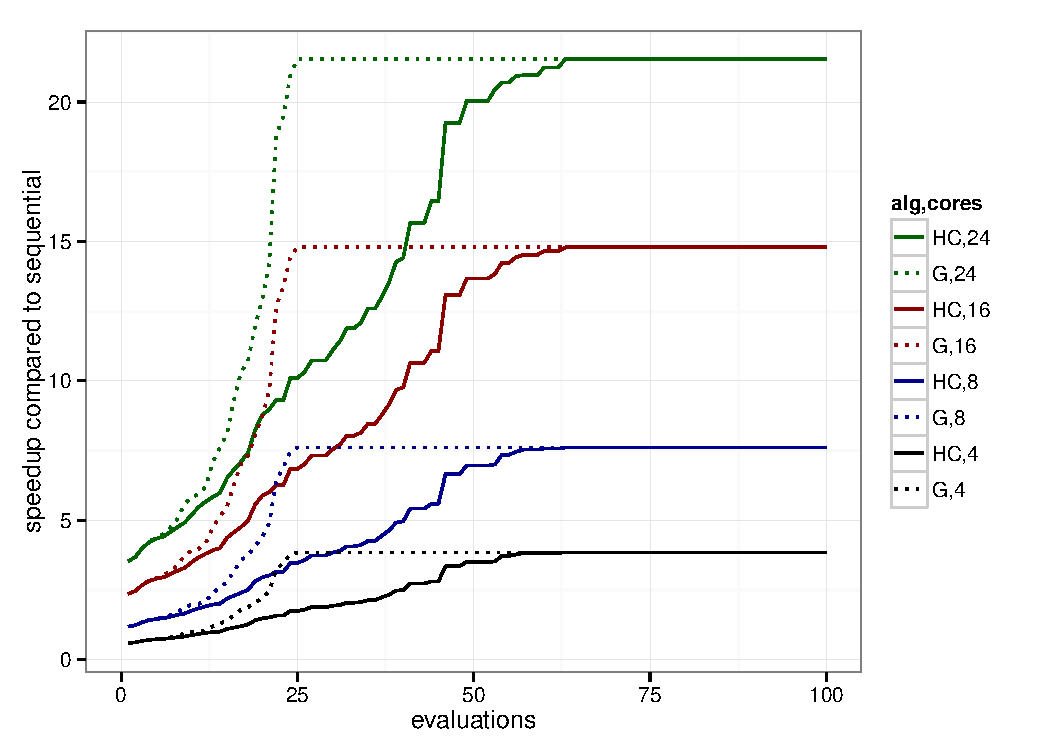
\includegraphics[scale=0.75]{Blind/Figures/speedup_by_evals_Queens2_allon_median.pdf}\\
(a) Queens2\\
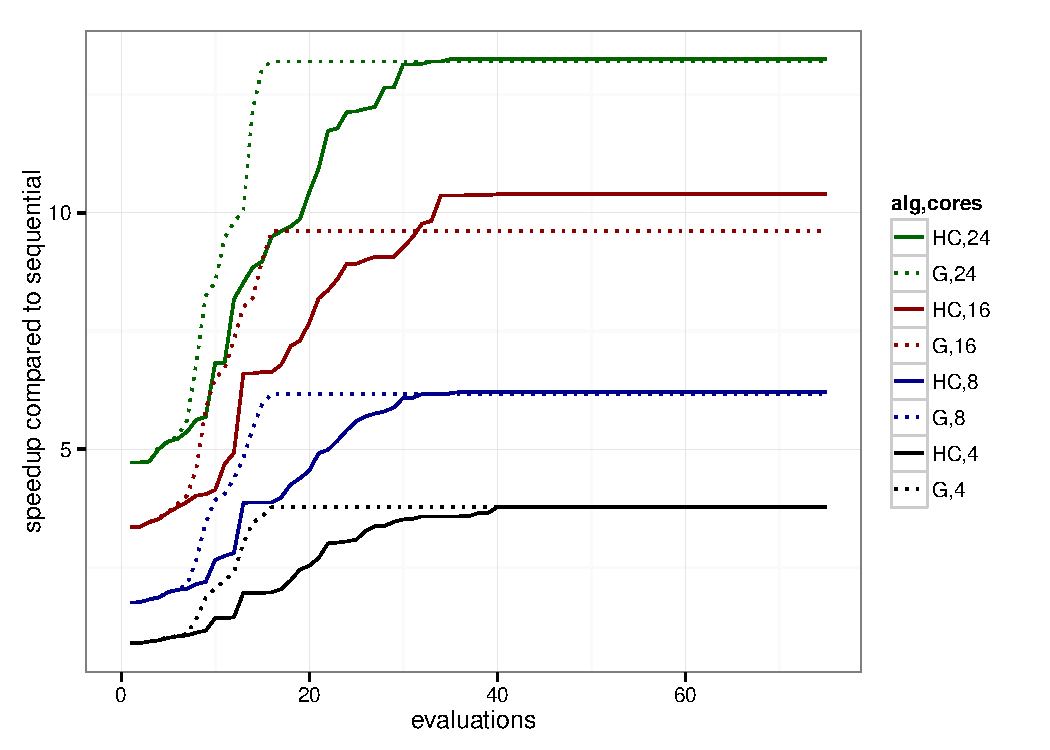
\includegraphics[scale=0.75]{Blind/Figures/speedup_by_evals_SodaCount_allon_median.pdf}\\
(b) SodaCount\\
\caption[Speedups against number of fitness evaluations for \texttt{Queens2} and \texttt{SodaCount}]{The speed-up, calculated as the ratio of the medians of the reduction counts, obtained so far by the algorithm plotted against the number of fitness evaluations. HC and G indicate the hill-climbing and greedy algorithm respectively, both using all-on initialisation. The numbers following the algorithm abbreviation indicate the number of cores.}
\label{fig:evals}
\end{figure}

\paragraph{RQ4}
For most benchmarks there is no statistically significant difference between
all-on and random initialisation.  For \verb|SodaCount|, the all-on
initialisation is slightly better for core counts of 4, 8, and 16.  This result
provides evidence that all-on initialisation may be beneficial, but requires
further investigation to confirm the generality.

\paragraph{}

The only results elided in Table \ref{tab:speedups} are the runtimes for the
greedy search with a random initialisation. This is because the random
initialisation produces inferior results in all cases and the same insight can
be gathered from studying the hill-climbing results for random initialisation.

    
        \section{Conclusions of Bitstring Searching}
        \label{sec:blind-Conclusion}
        We feel that this chapter has provided evidence that the combination of static
analysis and search can parallelise programs more effectively than through
static analysis alone. For some programs we are able to achieve close to linear
speed-ups which is as performant as can expected. These results are promising
for those looking to add iterative capabilities to their compiler but without
the ability to adapt the runtime system. By choosing an appropriate
representation of the available parallelism in a program, we are able to use
standard search techniques to search the possible parallel configurations.

The success of the greedy algorithm was somewhat surprising. It further
supports the idea that the vast majority of potential parallelism in any given
program does not make up for the overhead costs associated with creating and
managing that parallelism.

    
    \chapter{Profile Directed Search}
    \label{chap:prof-search}
    
        New things here.
        \label{sec:informed-search}
        \subsection{Iteration}

While we do record a variety of statistics, our current approach focuses on
reduction count as a guide to determine which \verb-par- sites are beneficial
to the program.  The reasoning is simple, our motivation for parallelism is to
do more work at once, so measuring the amount of work undertaken by each thread
is likely to be a good metric.

Because we record how productive each thread in a program is and we keep track
of which \verb-par- site created each thread, we can easily visualise how useful
each \verb-par- site is. Figure \ref{fig:sumHist} gives an overview of the health
of each \verb-par--site. For each site we record the total number of reductions
carried out. The plot shows us the statistics for this data with the median
(line), inter-quartile range (IQR, box), and $\pm1.5 * $IQR (whiskers).
Statistical outliers are shown as independent points. The \verb-par-sites that
only show a line as their plot either have only one child thread (the case for
\verb-par--site 1) or have little variance in the distribution of reduction
counts.

\begin{figure}
  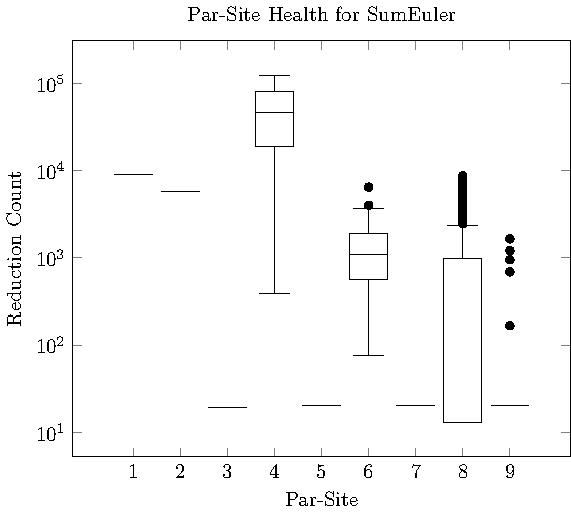
\includegraphics[width=\linewidth]{Informed/Figures/threadhealth.pdf}
\caption{Statistics on the number of reductions carried out by the threads a
\texttt{par} site sparks off}
\label{fig:sumHist}
\end{figure}

After every execution of the program, turn off the \verb'par' site whose threads
have the lowest average reduction count. In the case of the execution statistics
displayed in Figure \ref{fig:sumHist} we would disable \verb-par- site 2, allowing
us to avoid the overhead of all the unproductive threads it sparked off.  Then
repeat this process until switching a \verb'par' site off increases the overall
runtime of the program.

\section{Experimental Results}
\label{sec:results}

In this section we present some preliminary results and point out certain patterns
that appear in our data. 

First we introduce our benchmark programs and state the number of \verb-par-
sites that were introduced statically:

\subsection*{Overheads} Whether an expression is worthwhile to evaluate in
parallel is directly tied to \emph{cost} of creating a parallel task. In order
to account for this we ran all of our experiments with the simulated overhead
cost at 3 settings. We chose the upper and lower bounds based on benchmarking parallel
functions using the Criterion library \citep{criterion}.


For each program we set our runtime system to simulate 4, 8, and 16 cores.
First, let us examine Figure \ref{table10} which displays the results of setting
the cost of task creation to 10 reductions.

\begin{figure}[ht]
\centering
  \begin{tabular}{ |l||c c|c c|c c| }
    \hline
    Program & \multicolumn{2}{c|}{4-core} & \multicolumn{2}{c|}{8-cores} & \multicolumn{2}{c|}{16-cores} \\
    \hline
            & Runs & Final     & Runs & Final      & Runs & Final \\
    \hline
    SumEuler  & 6    & 3.77      & 6    & 6.84       & 6    & 10.27     \\
    Queens    & 5    & 1.30      & 5    & 1.37       & 5    & 1.41  \\
    Queens2   & 22   & 3.91      & 22   & 7.74       & 22   & 15.07   \\
    SodaCount & 3    & 2.42      & 3    & 4.72       & 3    & 8.95    \\
    Tak       & 1    & 3.39      & 1    & 6.79       & 1    & 13.58   \\
    Taut      & 4    & 1.00      & 0    & 1.00       & 9    & 1.00  \\
    MatMul    & 2    & 1.02      & 2    & 1.07       & 2    & 1.10   \\
    \hline
  \end{tabular}
\caption{Speedups relative to sequential computation when the cost of sparking
        a task is set to 10 reductions. The number of runs corresponds to the
        number of \texttt{par} sites that have been switched off.}
\label{table10}
\end{figure}

Already there are a few interesting results. \texttt{SumEuler} performs as expected and
manages to eliminate the majority of the introduced \verb-par- sites. Recalling
Figure \ref{sumLast}, the \verb-par-s that survive the iterative improvement
are the two in the \verb-main- function and the \verb-par- in \verb-mainListS2-.
The second \verb-par- in \verb-main- and the strategy \verb-mainListS2- are,
taken together, equivalent to applying \verb-parMap euler- over the input list.
When this program is parallelised explicitly, that \verb-parMap- is usually the
only addition to the program \citep{vGMachine}. It is reassuring that our
technique converges on the same result.

The two implementations of nQueens vary drastically in their improvement, with
the more symbolic solution (\texttt{Queens2}) achieving much better results. Search
problems are known to be problematic for techniques involving strictness
analysis and usually benefit from the introduction of \emph{speculative}
parallelism \citep{hammond2000research}.

\texttt{Taut} was chosen as a benchmark program specifically because the program (as
written) did not have many opportunities for parallelism. Had our technique
managed to find any useful parallelism, we would have been surprised.

MatMul is, to us, the most surprising of the results so far. Matrix
multiplication is famously parallelisable and yet our implementation
barely breaks even! Notice that of the 7 \verb-par- sites in MatMul, only
2 are being switched off. The \verb-par- setting that the iterative
improvement converged on was not the optimal setting (we know there is at least
2 superior settings). This convergence on local maxima is something we will
discuss in \S\ref{sec:conclusion}.

While the results in Figure \ref{table10} are revealing, it could be argued that
an overhead of 10 reductions to spark off a thread is unrealistically low.
Therefore we repeat the experiments with the more realistic 100 reduction
overhead (Figure \ref{table100}) and the pessimistic case of 1000 reduction
overheads (Figure \ref{table1000}).

\begin{figure}[ht]
\centering
  \begin{tabular}{ |l||c c|c c|c c| }
    \hline
    Program & \multicolumn{2}{c|}{4-core} & \multicolumn{2}{c|}{8-cores} & \multicolumn{2}{c|}{16-cores} \\
    \hline
            & Runs & Final     & Runs & Final      & Runs & Final \\
    \hline
    SumEuler  & 6    & 3.74      & 6    & 6.81       & 6    & 10.23     \\
    Queens    & 5    & 1.29      & 5    & 1.37       & 5    & 1.41  \\
    Queens2   & 22   & 3.83      & 22   & 7.57       & 22   & 14.76  \\
    SodaCount & 3    & 2.17      & 3    & 4.23       & 3    & 8.02    \\
    Tak       & 1    & 2.36      & 1    & 4.71       & 1    & 9.42   \\
    Taut      & 9    & 1.00      & 0    & 1.00       & 9    & 1.00  \\
    MatMul    & 2    & 0.93      & 2    & 1.06       & 2    & 1.09   \\
    \hline
  \end{tabular}
\caption{Speedups relative to sequential computation when the cost of sparking
        a task is set to 100 reductions. The number of runs corresponds to the
        number of \texttt{par} sites that have been switched off.}
\label{table100}
\end{figure}

The results in Figure \ref{table100} mostly align with what we would expect to
happen if creating a parallel task incurred higher overheads: we see reduced
speedup factors and adding more cores is less likely to benefit.

The key point to take away from this set of results is that while lower speedups
are achieved, the \emph{same} \verb-par- sites are eliminated in the same
number of iterations \footnote{Except for \texttt{Taut}, which in the 4-core case now
takes 9 runs to determine that there is no parallelism in the program.}.

Now we try the same experiment again but with the less realistic 1000 reduction
overhead to create a new thread.

\begin{figure}[ht]
\centering
  \begin{tabular}{ |l||c c|c c|c c| }
    \hline
    Program & \multicolumn{2}{c|}{4-core} & \multicolumn{2}{c|}{8-cores} & \multicolumn{2}{c|}{16-cores} \\
    \hline
            & Runs & Final     & Runs & Final      & Runs & Final \\
    \hline
    SumEuler  & 6    & 3.51      & 6    & 6.40       & 6    & 9.73     \\
    Queens    & 5    & 1.26      & 5    & 1.35       & 5    & 1.40  \\
    Queens2   & 22   & 3.14      & 22   & 6.22       & 22   & 12.18  \\
    SodaCount & 12   & 1.85      & 3    & 2.08       & 1    & 1.39    \\
    Tak       & 1    & 0.57      & 1    & 1.15       & 1    & 2.32   \\
    Taut      & 12   & 1.00      & 12   & 1.00       & 7    & 1.00  \\
    MatMul    & 5    & 1.00      & 5    & 1.00       & 5    & 1.01   \\
    \hline
  \end{tabular}
\caption{Speedups relative to sequential computation when the cost of sparking
        a task is set to 1000 reductions. The number of runs corresponds to the
        number of \texttt{par} sites that have been switched off.}
\label{table1000}
\end{figure}

While the speedups are now much more moderate (when there is a speedup at all)
these results are interesting for a few reasons.

In particular, the number of cores now has a greater influence on how many
\verb-par- sites are worthwhile.  \texttt{SodaCount}, for instance, now eliminates 12 of
its 15 \verb-par- annotations in the case of 4-core execution. This fits with
our intuition that when there are fewer processing units the threads require
coarser granularity to be worthwhile. In the cases of 8 and 16-core executions
we observe that fewer \verb-par- sites are disabled, reinforcing this
intuition.

MatMul also sees a jump in the number of disabled \verb-par- sites. Sadly, this
results in even worse performance for MatMul, which should be a highly
parallelisable program.

\subsection*{Static vs. Iterative}

While the results presented in Informed/Figures \ref{table10}, \ref{table100}, and
\ref{table1000} are promising for preliminary results they are based on an
admittedly simple search heuristic. Part of our argument is that static analysis
\emph{alone} is not sufficient for good gains from implicit parallelism. Figure
\ref{fig:iters} presents a selection of results that show how the iterative
improvement affects the static placement of \verb-par- annotations.

Even in the cases where the final speedup is lower than anticipated, such as
\texttt{Queens} in Figure \ref{fig:iterQueens}, the program still benefits from the
iterative improvement. \texttt{Queens2} sees the highest payoff from iterative
improvement. Many of the \verb-par-s introduced by the static analysis
do not contribute significantly to the computation even though it is
semantically safe to introduce them. The iterative loop converges on the few
\verb-par- sites that make a significant difference.

\begin{figure}[h]
    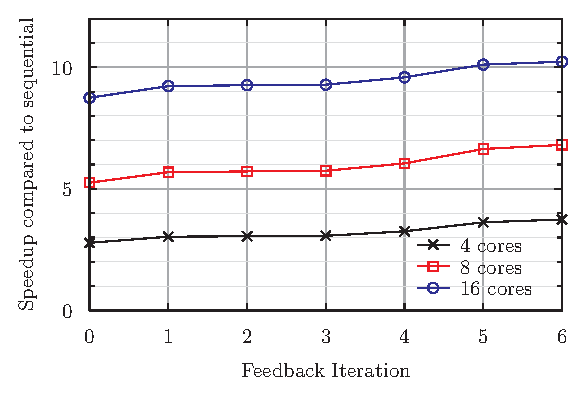
\includegraphics[scale=0.75]{Informed/Figures/IterSum.eps}
    \caption[SE]{\texttt{SumEuler} speedup}
    \label{fig:iterSum}
\end{figure}
\begin{figure}[h]
    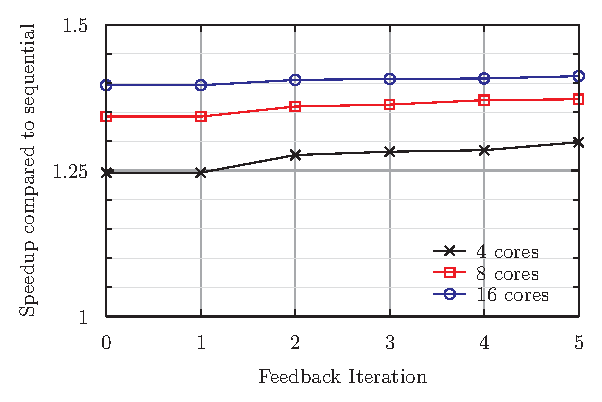
\includegraphics[scale=0.75]{Informed/Figures/IterQueens.eps}
    \caption[Q]{\texttt{Queens} speedup}
    \label{fig:iterQueens}
\end{figure}

\begin{figure}[h]
    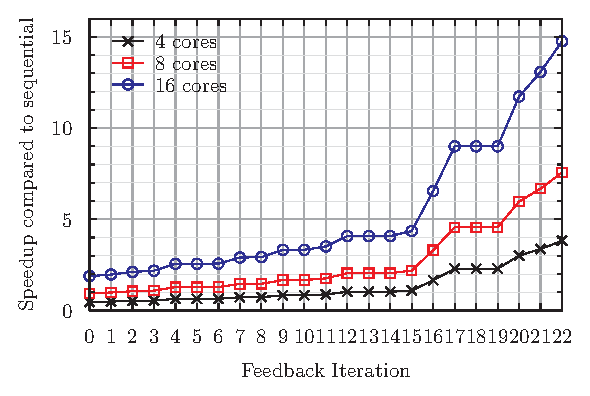
\includegraphics[scale=0.75]{Informed/Figures/IterQueens2.eps}
    \caption[Q2]{\texttt{Queens2} speedup}
    \label{fig:iterQueens2}
\end{figure}
\begin{figure}[h]
    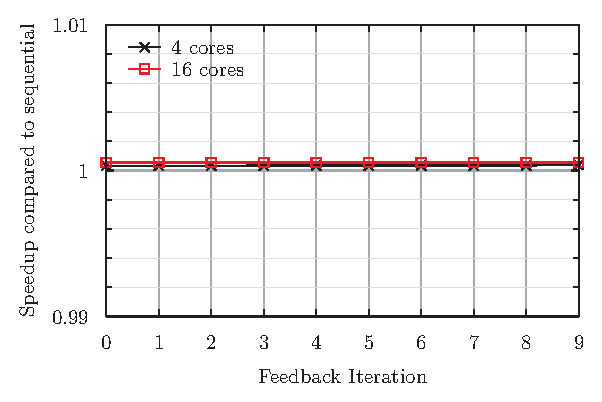
\includegraphics[scale=0.75]{Informed/Figures/IterTaut.eps}
    \caption[T]{\texttt{Taut} speedup}
    \label{fig:iterTaut}
\end{figure}


\subsection*{Comparison to GHC}

While the results above are encouraging we would like to see how the resulting
programs perform when compiled by a modern high-performance Haskell compiler.
To do this we extract the final \verb-par- settings from each program and
translate that to Haskell suitable for compilation by GHC.

For the versions parallelised by hand we use the \verb-par- placements found
in the literature \citep{vGMachine, runciman1994profiling}.

\begin{figure}[ht]
\centering
  \begin{tabular}{ |l||c c| }
    \hline
    Program & \multicolumn{2}{c|}{4-core} \\
    \hline
            & Hand   & Auto         \\
    \hline
    SumEuler  & 3.32    & 3.31      \\
    Queens    & 1.76    & 0.97      \\
    Queens2   & 2.29    & 0.61     \\
    SodaCount & 1.25    & 0.64      \\
    Tak       & 1.77    & 1.64      \\
    MatMul    & 1.75    & 0.80      \\
    \hline
  \end{tabular}
\caption{Speedups compared to the sequential program as compiled by GHC for both
         manually and automatically parallelised versions}
\label{tableGHC}
\end{figure}

As Table \ref{tableGHC} makes clear, the results are not impressive. In fact,
except for \verb-SumEuler- and \verb-Tak-, all of the parallel benchmarks
performed \emph{worse} than their sequential counterparts.

However, we feel that not all hope is lost. There are a few recurring issues in
the generated program. A common issue is that the generated strategies will not
be what forces the evaluation of a value. Take the following example as an
illustration

\begin{verbatim}
foo n = let ys = gen n n
        in par (tailStrict1 ys) (bar ys)

tailStrict1 xs = case xs of
    y:ys -> tailStrict1 ys
    []   -> ()
\end{verbatim}

In the function \verb-foo- we spark off a strategy that is meant to force the
spine of the list \verb-ys-, the catch is that GHC's \verb-par- is fast enough
for \verb-bar ys- to be what forces the evaluation of \verb-ys-. So we're
paying the overhead and reaping none of the benefits. In some programs changing
a \verb-par- like the one found in \verb-foo- to a \verb-seq- is enough to solve the
issue and make the parallel version competitive with the manually parallelised version.



\section{Conclusions}
\label{sec:conclusion}


We hope we have motivated the key design choices and ideas behind our compiler:
utilising defunctionalisation in \S\ref{sec:defunct}, and the use of
projections over other strictness analysis methods in \S\ref{sec:strictness}.
Moreover, that we have shown that there is a natural correspondence between
projections and strategies \S\ref{sec:proAndStrat} that allows us to generate
parallel strategies from the results of our strictness analysis.

While projection-based strictness analysis does provide a useful foundation for
the introduction of parallelism, the results in \S\ref{sec:results} show that
static analysis alone does not provide the desired speedups. Additionally,
Table \ref{tableGHC} shows that determining \verb-par--site health by reduction
count alone is too naive. Thread collisions that may not happen on a simulated
system are able to significantly hamper parallel performance and should be
taken into account.

\subsection{Related Work}

\subsection*{Hinze's Work on Projections} 

Much of the early work on strictness
analysis as a means to achieve implicit parallelism focused on the abstract
interpretation approach because the work on projections had not been fully
developed when implicit parallelism was a more active research area. In
particular, the work on the ``Automatic Parallelization of Lazy Functional
Programs'' \citep{hogen1992automatic} only used two and four-point domains (as
described in \citep{wadler1987strictness}) in their strictness analysis. This
limits the ability of the compiler to determine the neededness of more complex
structures.

Hinze's work on projection-based strictness analysis came after work on implicit
parallelism fell out of favour \citep{hinze1995projection, hammond2000research}. To
our knowledge we are the first to apply this work to the implicit parallelism.

\subsection{Comparison to Heuristic Search}

In the previous chapter we explored using two heuristic search algorithms to
accomplish our iterative step. While the results were promising, the ability to
examine profile data should not be underestimated. The first benefit is that
our search is guaranteed to be linear \emph{in the worst case} and usually
sub-linear, whereas even the greedy algorithm required exactly linear time.

As the programs grow larger the combinatorial explosion for the hill-climbing
will become more and more detrimental. For the hill-climbing algorithm to
terminate all neighbors to the current candidate must be explored. This means
that when a program has twenty \verb|par| sites, the \emph{last} iteration of
the hill-climbing algorithm will require twenty evaluations of the program! The
profile based technique's ability to guarantee that this program will require
\emph{at most} twenty iterations is a huge advantage.



\part{Conclusions and Future Directions}
\label{part:conclusion}

    \chapter{Future Directions}
    \label{chap:future}
    
        One of the main motivators of this work was the lack of attention implicit
parallelism has been receiving in the functional programming community.  Early
on, functional programmers were optimistic about the feasibility and benefits
of systems designed to exploit the inherent parallelism in our programs.  The
software and hardware ecosystem has changed beneath our feet since the 80's and
90's. Increasingly, software companies and developers often prioritise
developer productivity over software performance \citep{codingHorror}. The
exploitation of implicit parallelism will allow developers to regain
\emph{some} of the performance without the cost of developer time.

One of our aims with this work was to show that despite setbacks in the
past, there are still techniques and analyses worth exploring in this
research area.  We therefore turn our attention to the future and discuss some
of the possible avenues of exploration.

\subsection*{Plan of the Chapter}

There are many possible extensions and improvements that can be made to our
general technique. The most direct would be to use the runtime information for
function specialisation, similar to what we already do for the different
demands on a function in Section \ref{sec:specialiseDemand}. We discuss this
idea in Section \ref{sec:specialiseDepth}.

This thesis is predicated on the idea that implicit parallelism is our goal,
and we still believe that this is a worthy pursuit. But it does not have to be
\emph{limited to} implicit parallelism. There may be situations where the programmer
would like to specify that certain expressions are evaluated in parallel. We
explore what such hybrid systems might look like in Section \ref{sec:hybrid}.

It is also possible that the demand properties of a program would be useful in
identifying pipeline-parallelism automatically. Section \ref{sec:autoPipe}
explores how one might design such a system. 

    
        \section{Specialising on \underline{\hspace{2cm}}}
        In our implementation we specialised functions in two ways: higher-order to
first-order and \verb|par| placement based on varied demands. There are, of
course, many forms of specialisation that could be added: monomorphisation,
call-pattern specialisation, and even specialisation to some depth of a
recursive function. 

%When dealing with parallel programs, it is easy to think of
%examples where a polymorphic function may be suitable for parallelism when
%instantiated on one type, but not another. This is particularly true of bounded
%polymorphism in the form of typeclasses as found in Haskell
%\citep{haskellReport}. An overloaded \<size\> function may benefit from having
%its argument evaluated in parallel for one type (binary trees for example) and
%not for another
%
% I don't think the above idea holds water... If we have an overloaded function
% than it's individual instances are the things that will have the parallelism
% and even if not. The calls to `size` will _each_ have their own par sites,
% which can be turned off individually.

When writing parallel programs we often write recursive functions, particularly
divide-and-conquer algorithms, to take into account how deep into a
computation a call is. This allows the program to avoid the creation of
parallel threads when the computation is obviously (to the programmer) not
worthwhile. An example of this was shown in Section \ref{sec:parAndSeq} with
our definition of \<quicksort\>. This pattern is not only limited to
parallelising the more `shallow' levels of the computation and then switching to a
sequential version. It is possible that the leaves of a computation are the
expensive part, and to limit the number of generated
threads, one should begin with a sequential version and switch to a parallelised
version below some depth. The general shape of the technique is drawn in Figure
\ref{fig:compDepth}.

\begin{figure}[t]
\centering
\begin{tikzpicture}[
    level 1/.style={sibling distance=6cm},
    level 2/.style={sibling distance=3cm},
    level 3/.style={sibling distance=1.5cm},
    level 4/.style={sibling distance=0.75cm}]
  \node [hassef] {}
    child{ node [hassef] {} 
            child{ node [hassef] {} 
                            child{ node [hasse] {}
                                            child{ node [hasse] {}}
                                            child{ node [hasse] {}}
                                 }
                            child{ node [hasse] {}
                                            child{ node [hasse] {}}
                                            child{ node [hasse] {}}
                                 }
            }
            child{ node [hassef] {}
                            child{ node [hasse] {}
                                            child{ node [hasse] {}}
                                            child{ node [hasse] {}}
                                 }
                            child{ node [hasse] {}
                                            child{ node [hasse] {}}
                                            child{ node [hasse] {}}
                                 }
            }               
    }
    child{ node [hassef] {}
            child{ node [hassef] {} 
                            child{ node [hasse] {}
                                            child{ node [hasse] {}}
                                            child{ node [hasse] {}}
                                 }
                            child{ node [hasse] {}
                                            child{ node [hasse] {}}
                                            child{ node [hasse] {}}
                                 }
            }
            child{ node [hassef] {}
                            child{ node [hasse] {}
                                            child{ node [hasse] {}}
                                            child{ node [hasse] {}}
                                 }
                            child{ node [hasse] {}
                                            child{ node [hasse] {}}
                                            child{ node [hasse] {}}
                                 }
            }
    }
  ;
  \draw [cyan, dashed, ultra thick] (-5.2,-3.6) -- (5.2,-3.6);
  \node [above, cyan] at (0,-3.6) {$d$};
\end{tikzpicture}
\caption{A tree representation of a recursive computation}
\label{fig:compDepth}
\end{figure}

Given some depth of the computation $d$ (usually measured in the number of
recursive calls) for the function \<f\>, the shaded nodes represent calls to one
specialised form of \<f\> and the unshaded nodes represent another specialisation
of \<f\>. We can attain these two versions simply with the following transformation

\begin{haskell}
f x = \hsinf{\<e\>} \(\phantom{space}\) \Longrightarrow
\(\phantom{space}\) &f_{1} d x &= \hsif{d > depth}{%
                                                     f x}{%
                                                     \ \hsinf{\<e_{[f \(\mapsto\) f1 (d + 1)]}\>}} \\
\end{haskell}

All original calls to \<f\> in the source program become \<f_{1} 0\> and only
below a certain depth do we begin to call the original function. What benefit does
this give us? Now any \verb|par| sites in \<f\> are duplicated in \<f_{2}\>
and can be switched independently based on the depth. This gives the iterative
step the flexibility to switch off the \verb|par|s for the levels of the call
tree that are not worthwhile to perform in parallel.

In order to choose an appropriate value for \<depth\> in \<f_{1}\> the runtime
system must be equipped with some proxy for call-depth. This could take the form
of something similar to what is used to get stack traces for lazy functional languages
\citep{AllwoodStack}.

We hypothesise that the value of \<depth\> in \<f_{1}\> does not have to be
perfect on the first attempt. By ensuring that a \emph{reasonable} \<depth\> is
chosen the compiler can then determine which \verb|par|s, the ones in \<f_{1}\>
or the ones lower in the call-depth in \<f\>, should remain on. Once the on/off
decisions have been made the compiler could attempt to \emph{tune} the value of
\<depth\>.

\subsection{Knowing When to Specialise on Depth}

A subtle point is knowing \emph{when} this form of specialisation is useful.
As with the main argument of this thesis, we would use both static and dynamic
information about the program.  We believe that candidate functions for
specialisation on depth must exhibit \emph{at least} the following properties:

\begin{enumerate}
    \item The function must be recursive
    \item The function must parallelise a recursive call to itself
    \item The \verb|par| site accomplishing the above has a wide distribution
            of \verb|par| health (as exemplified by \verb|par| site \#8 in
            \ref{fig:sumHist})
\end{enumerate}

We believe that for large scale programs, specialising on depth will be
necessary as divide-and-conquer algorithms are quite common.

    
        \section{Hybrid Approaches}
        We have presented our work as being fully automated and requiring no
intervention by the programmer, but if we loosen that requirement on
our technique we may be able to find a fruitful `middle-ground' between
fully-automated parallelism and programmer effort.

\subsubsection{Super Strategies}

One technique that we find promising is the idea of an automatic strategy.

It is common for a programmer to know that an algorithm should be
parallelisable but does not want to invest the effort in parallelising the code
by hand. A `super-strategy' would allow the programmer to annotate the program,
telling the compiler `this expression should be parallelisable', but without
specifying how. This saves the compiler from searching for parallelism
throughout the whole program and iterating over the large resulting search
space and instead focus its static analysis and iteration to the annotated
expression.

This could be exposed to the programmer with an interface similar to parallel
strategies \citep{strategies}.

Something along the lines of:

\begin{haskell}
\hsinf{expression Alice would like to parallelise} `using` autoStrat
\end{haskell}

Or more conventionally:

\begin{haskell}
autoPar \hsinf{expression Alice would like to parallelise}
\end{haskell}

The auto-strategy would still use the demand information available at compile
time, and proceed in the manner outlined in this thesis, but the compiler would
benefit from a much reduced search space.

    
        \section{Automating Pipeline Parallelism}
    
    
    \chapter{Conclusions}
    \label{chap:conclusions}
    
        And.... we're done.

%%%%%%%%%%%%%%%%%%%%%%%%%%%%%%%%%%%%%%%%%%%%%%%%%%%%%%%%%%%%%%%%
%%%%%%%%%%%%%%%%%%%%%%%%%% APPENDICES %%%%%%%%%%%%%%%%%%%%%%%%%%
%%%%%%%%%%%%%%%%%%%%%%%%%%%%%%%%%%%%%%%%%%%%%%%%%%%%%%%%%%%%%%%%

\begin{appendices}

\chapter{Benchmark Programs}


\end{appendices}

\listoftodos[Notes]

\if@openright
  \cleardoublepage
\else
  \clearpage
\fi

\bibliography{literature}
\bibliographystyle{plainnat}

\end{document}
